\documentclass[%
%%% PARA ESCOLHER O ESTILO TIRE O SIMBOLO %(COMENT?RIO)
%SemVinculoColorido,
%SemFormatacaoCapitulo,
%SemFolhaAprovacao,
%SemImagens,
%CitacaoNumerica, %% o padr?o ? cita??es tipo autor-data
%PublicacaoDissOuTese, %% (? tambem o "default") com ficha catal. e folha de aprova?eo em branco. 
%			Caso tenha lista de s?mbolos e lista de siglas e abreviaturas retirar os comentarios 
%			dos arquivos siglas.tex e abreviaturasesiglas.tex. Retirar tambem os coment?rios indicados nesse 
%			arquivo, nos includes
%PublicacaoArtigoOuRelatorio, %% texto sequencial, sem quebra de p?ginas nem folhas em branco
%PublicacaoProposta, %% igual tese/disserta?eo, mas sem ficha catal. e fol. de aprov.
%PublicacaoLivro, %% com capitulos
%PublicacaoLivro,SemFormatacaoCapitulo, %% sem capitulosl
english,portuguese %% escolha o idioma (brazilian, portuguese, american, british, english)
%,LogoINPE	%% comentar essa linha para fazer aparecer o logo do Governo
]{tdiinpe}
%]{../../../../../iconet.com.br/banon/2008/03.25.01.19/doc/tdiinpe}

% PARA EXIBIR EM ARIAL TIRAR O COMENT?RIO DAS DUAS LINHAS SEGUINTES
%\renewcommand{\rmdefault}{phv} % Arial
%\renewcommand{\sfdefault}{phv} % Arial

% PARA PUBLICACAO:
% renomear o arquivo: abnt-alf.bst para abnt-alfportuguese.bst
% renomear o arquivo: abnt-alfenglish.bst para abnt-alf.bst


%%%%%%%%%%%%%%%%%%%%%%%%%%%%%%%%%%%%%%%%%%%%%
%%% Pacotes j? previamente carregados:      %
%%%%%%%%%%%%%%%%%%%%%%%%%%%%%%%%%%%%%%%%%%%%%%%%%%%%%%%%%%%%%%%%%%%%%%%%
%%% ifthen,calc,graphicx,color,inputenc,babel,hyphenat,array,setspace, %
%%% bigdelim,multirow,supertabular,tabularx,longtable,lastpage,lscape, %
%%% rotate,caption2,amsmath,amssymb,amsthm,subfigure,tocloft,makeidx,  %
%%% eso-pic,calligra,hyperref,ae,fontenc                               %
%%%%%%%%%%%%%%%%%%%%%%%%%%%%%%%%%%%%%%%%%%%%%%%%%%%%%%%%%%%%%%%%%%%%%%%%
%%% insira neste campo, comandos de LaTeX %%%
%%% \usepackage{_exemplo_}
% etc.
%%%%%%%%%%%%%%%%%%%%%%%%%%%%%%%%%%%%%%%%%%%%%

%\watermark{Revisao de seu documento
%% comente este comando quando for gerar a versao final
\usepackage{listings}
\usepackage{hyphenat}
\usepackage{rotating}
\usepackage{dsfont}
\usepackage{listings}
\usepackage{amsmath}

\lstset{numbers=left,
	extendedchars=\true, % permite acentos
	inputencoding=latin1, 
	commentstyle=\it, % deixa os comentario
	stringstyle=\bf, 
	belowcaptionskip=5pt, 
	numbers=left, 
	stepnumber=1, 
	firstnumber=1, % primeira linha
	numberstyle=\tiny, % tamanho da fonte da numeracao
	breaklines=true, % permitir quebra de linha
	frame=tb, % borda em cima e em baixo
	basicstyle=\footnotesize, % estilo basico
	keywordstyle=\color{blue},
	stringstyle=\ttfamily, 
	showstringspaces=false, 
	mathescape, 
	tabsize=3  
}
\renewcommand{\lstlistingname}{C�digo-Fonte}
\renewcommand{\lstlistlistingname}{Lista de Listagens}
\newcolumntype{C}[1]{>{\centering\let\newline\\\arraybackslash\hspace{0pt}}m{#1}}

%%%%%%%%%%%%%%%%%%%CAPA%%%%%%%%%%%%%%%%%%%%%%%%%%%%%%%%
%\serieinpe{INPE-NNNNN-TDI/NNNN} %% n�o mais usado

\titulo{Extra��o de estradas em imagens \emph{SAR} aerotransportadas: Uma abordagem baseada em Modelo de Contorno Ativo com o uso de semeador 
semiautom�tico}
\title{Roads center-axis extraction in airborne SAR images: An approach based in Active Contour Model with the use of semi-automatic seeding} %% 
\author{Rodolfo Georjute Lotte} %% coloque o nome do(s) autor(es)
\descriccao{Disserta��o de Mestrado do Curso de P�s-Gradua��o em Computa��o Aplicada, orientada pelo Dr. Sidnei Jo�o Siqueira Sant'Anna, Dra. Cl�udia Maria de Almeida, 
Dra. Corina da Costa Freitas e Dr. Jos� Demi�sio Sim�es da Silva}%, aprovada em dd de m�s por extenso de aaaa.}
\repositorio{aa/bb/cc/dd} %% reposit�rio onde est�o depositado este documento - na omiss�o, ser�o preenchido pelo SID
\tipoDaPublicacao{TDI}	%% tipo da publica��o (NTC, RPQ, PRP, MAN, PUD, TDI, TAE e PRE) na aus�ncia do n�mero de s�rie INPE, caso contr�rio deixar vazio
\IBI{xx/yy} %% IBI (exemplo: J8LNKAN8PW/36CT2G2) quando existir, caso contr�rio o nome do reposit�rio onde est�o depositado o documento

\date{2012}%ano da publica��o

%%%%%%%%%%%%%%%%%%%%%%%%%%VERSO DA CAPA%%%%%%%%%%%%%%%%%%%%%%%%%%%%%%%%%%%%%%%%%%%%%%%
\tituloverso{\vspace{-0.9cm}\textbf{\PublicadoPor:}}
\descriccaoverso{Instituto Nacional de Pesquisas Espaciais - INPE\\
Gabinete do Diretor (GB)\\
Servi�o de Informa��o e Documenta��o (SID)\\
Caixa Postal 515 - CEP 12.245-970\\
S�o Jos� dos Campos - SP - Brasil\\
Tel.:(012) 3945-6923/6921\\
Fax: (012) 3945-6919\\
E-mail: {\url{pubtc@sid.inpe.br}}
}

\descriccaoversoA{\textbf{\ConselhoDeEditoracao:}\\
\textbf{\Presidente:}\\
Dr. Gerald Jean Francis Banon - Coordena��o Observa��o da Terra (OBT)\\
\textbf{\Membros:}\\
Dra� Inez Staciarini Batista - Coordena��o Ci�ncias Espaciais e Atmosf�ricas (CEA)\\
Dra� Maria do Carmo de Andrade Nono - Conselho de P�s-Gradua��o \\
Dra� Regina C�lia dos Santos Alval� - Centro de Ci�ncia do Sistema Terrestre (CST)\\
Marciana Leite Ribeiro - Servi�o de Informa��o e Documenta��o (SID)\\
Dr. Ralf Gielow - Centro de Previs�o de Tempo e Estudos Clim�ticos (CPT)\\
Dr. Wilson Yamaguti - Coordena��o Engenharia e Tecnologia Espacial (ETE)\\
Dr. Hor�cio Hideki Yanasse - Centro de Tecnologias Especiais (CTE)\\
\textbf{\BibliotecaDigital:}\\
Dr. Gerald Jean Francis Banon - Coordena��o de Observa��o da Terra (OBT)\\
Marciana Leite Ribeiro - Servi�o de Informa��o e Documenta��o (SID)\\
%Jefferson Andrade Ancelmo - Servi�o de Informa��o e Documenta��o (SID)\\
%Simone A. Del-Ducca Barbedo - Servi�o de Informa��o e Documenta��o (SID)\\
%Deicy Farabello - Centro de Previs�o de Tempo  e Estudos Clim�ticos (CPT)\\
\textbf{\RevisaoNormalizacaoDocumentaria:}\\
Marciana Leite Ribeiro - Servi�o de Informa��o e Documenta��o (SID) \\
%Maril�cia Santos Melo Cid - Servi�o de Informa��o e Documenta��o (SID)\\
Yolanda Ribeiro da Silva Souza - Servi�o de Informa��o e Documenta��o (SID)\\
\textbf{\EditoracaoEletronica:}\\
Viv�ca Sant'Ana Lemos - Servi�o de Informa��o e Documenta��o (SID)\\
}
%%%%%%%%%%%%%%%%%%%FOLHA DE ROSTO

%%%%%%%%%%%%%%%FICHA CATALOGR�FICA
%% N�O PREENCHER - SER� PREENCHIDO PELO SID

\cutterFICHAC{Cutter}
\autorUltimoNomeFICHAC{Lotte, Rodolfo Georjute} %% exemplo: Fuckner, Marcus Andr�
\autorAbreviadoFICHAC {} %% N�o usado - deixar vazio
\tituloFICHAC{Extra��o de estradas em imagens \emph{SAR} aerotransportadas: Uma abordagem baseada em Modelo de Contorno Ativo com o uso de semeador 
semiautom�tico}
\instituicaosigla{INPE}
\instituicaocidade{S�o Jos� dos Campos}
\paginasFICHAC{\pageref{numeroDeP�ginasDoPretexto} + \pageref{LastPage}} %% n�mero total de p�ginas
%\serieinpe{INPE-00000-TDI/0000} %% n�o mais usado
\palavraschaveFICHAC{1.~\emph{Snakes}. 2.~extra��o de estradas 3.~semea��o semiautom�tica. 4.~imagem de radar. I.~\mbox{T��tulo}.} %% recomenda-se pelo menos 5 palavras-chaves - \mbox{} � para evitar hifeniza��o 
\numeroCDUFICHAC{000.000} %% n�mero do CDU 

% Nota da ficha (para TD)
\tipoTD{Disserta��o} % Disserta��o ou Tese
\cursoFA{Mestrado em Computa��o Aplicada}
\instituicaoDefesa{Instituto Nacional de Pesquisas Espaciais}
\anoDefesa{2012} % ano de defesa 
\nomeAtributoOrientadorFICHAC{Orientador}	% pode ser: Orientador, Orientadora ou Orientadores
\valorAtributoOrientadorFICHAC{Corina da Costa Freitas} % nome(s) completo(s)

%%%%%%%%%%%%%%%FOLHA DE APROVAÇAO PELA BANCA EXAMINADORA
\tituloFA{\textbf{ATEN��O! A FOLHA DE APROVA��O SER� INCLU�DA POSTERIORMENTE.}}
%\cursoFA{\textbf{}}
\candidatoOUcandidataFA{}
\dataAprovacaoFA{}
\membroA{}{}{}
\membroB{}{}{}
\membroC{}{}{}
\membroD{}{}{}
\membroE{}{}{}
\membroF{}{}{}
\membroG{}{}{}
\ifpdf

%%%%%%%%%%%%%%N�VEL DE COMPRESS�O {0 -- 9}
\pdfcompresslevel 9
\fi
%%% define em 80% a largura das figuras %%%
\newlength{\mylenfig} 
\setlength{\mylenfig}{0.8\textwidth}
%%%%%%%%%%%%%%%%%%%%%%%%%%%%%%%%%%%%%%%%%%%

%%%%%%%%%%%%%%COMANDOS PESSOAIS
\newcommand{\vetor}[1]{\mathit{\mathbf{#1}}}
 %% funcoes pertinentes no arquivo configuracao.tex

\makeindex  %% nao alterar, gera INDEX, caso haja algum termo indexado no texto

\begin{document} 

\maketitle 

%%% Comente as linhas opcionais abaixo caso nao as deseje
\begin{epigrafe}
   \textit{\large\textquotedblleft Storms make trees take deeper roots\textquotedblright.}
   \\
   \vspace{1cm}  
   \hspace{4cm} \emph{\textsc{Dolly Parton}}
    
%    \textit{\large``Somewhere, something incredible is waiting to be known''.}
%    \vspace{1cm}  
%    \hspace{4cm} \emph{\textsc{Carl Sagan}}
%   \textit{\large``If you do not change direction, you may end up where you are heading''.}
%   \vspace{1cm}  
%   \hspace{4cm} \emph{\textsc{Lao Tzu}}
\end{epigrafe}
 %% Opcional
\begin{dedicatoria}
\hypertarget{estilo:dedicatoria}{}

\newcommand{\mytext}{To my parents Raul and Z�lia, and my sister, Cl�udia}

	\ifcalligra %% fonte calligra presente nas vers�es mais novas do MiKTeX (>= 2.4)
	  \calligra\Large \mytext %% exemplo usando estilo de fonte caligr�fica, caso haja
	\else
		\itshape\Large \mytext 
	\fi

\end{dedicatoria}
 %% Opcional
\begin{agradecimentos}
  We create an imaginary show inside our heads, a show that involves more frustrations than the hope of reaching our goal. They are daily struggles, daily failures, so many blows that at first we thought we had lost all this time, but actually, it has been taking you to the highest point, to the point of seeing that small failures were all part of the same gear, the conquest. The energy that always moved me was the disbelief in my work, the lack of support, the disloyalty from part of this department, and the fear of not being able to conclude. But that gear was also \textquotedblleft lubricated\textquotedblright~so many times by faith, family, innumerable friends, places, travels, and so many other events that made things a little less painful. And it is for these people that I toast and dedicate this work today. Thank you to look with me this brand new horizon.    
  % Criamos um espet�culo dentro de nossas cabe�as, um espet�culo que envolve mais frusta��es do que a esperan�a de atingir nosso objetivo. S�o lutas di�rias, falhas di�rias, tantas pancadas que, no �nicio, pensamos ter perdido todo esse tempo, mas que na realidade, lhe levava ao ponto mais alto, ao ponto de enxergar que as pequenas falhas eram todas pe�as da mesma engrenagem, a da conquista. A energia que sempre movimentou-me foi a descren�a em meu trabalho, a falta de suporte, a deslealdade e descaso de parte deste departamento, e o medo de n�o conseguir. Mas essa engrenagem tamb�m foi ``lubrificada'' tantas vezes pela f�, fam�lia, pelos in�meros amigos, lugares, viagens e tantos outros acontecimentos que tornaram as coisas um pouco menos penosas. E s�o por essas pessoas que brindo e dedico esse trabalho hoje. Obrigado por enxergarem comigo meu mais novo horizonte.
  
  During my PhD, I had the chance to experience the guidance, friendship, support, criticism, and love of incredible people. Everyone who shared this energy played key roles in my evolution and what I am today. Above all, God and Nossa Senhora de Aparecida. Faith and science, the most famous paradox. Lord did not give me the thesis or health, but faith on you will always be the fuel of my determination and hope.
  %Durante o per�odo de meu Doutorado, tive a chance de experienciar a orienta��o, amizade, suporte, cr�tica e amor de pessoas incr�veis. Todos que compartilharam desta energia, tiveram pap�is fundamentais em minha evolu��o e do que sou hoje. Sobretudo, � Deus e � Nossa Senhora da Aparecida. O famoso paradoxo: f� e ci�ncia. O Senhor n�o me deu a tese ou sa�de, mas a f� em ti ser� sempre o combust�vel em minha determina��o. 
  
  A special thanks to the great sponsors of this work, my parents, Raul and Z�lia, and my sister, Claudia. I can not imagine this work, or anything else, being done without your cooperation or presence. Thanks for everything.
  %Um agradecimento especial aos grandes incentivadores e \textquotedblleft patriocinadores emocional\textquotedblright$~$deste trabalho, meus pais, Raul e Z�lia, e minha irm�, Cl�udia. N�o consigo imaginar este trabalho, ou qualquer outra coisa, sendo realizado sem coopera��o ou presen�a de voc�s. Obrigado por tudo. 
  
  To the great INPE, which has hosted me since the master's degree in Applied Computing (2010), to its inspiring infrastructure and environment. To the eternal friends of the postgraduate class in Remote Sensing of 2014, with affection to my friends Aline Jacon, Ana Pessoa, Bruna Pechini, Cesare Neto, David Fran�a, Denis Mariano, Henrique Cassol, Jaidson Becker, Jo�o Felipe , Jo�o Bosco, Ranieli dos Anjos, Sacha Siani and all others who were with me. My friends from Hannover, in special Alexander Schunert, Lukas Schack and Joachim Niemeyer. To my dear friends and advisors Dr. Luiz Arag�o and Dr. Yosio Shimabukuro, for having taken this work already underway, for believing, for cooperation and friendship until the end. Dr. Elisabete Moraes, my academic mother and great friend. Thank you for embracing the cause so many times, for understanding and for struggling with me. This work is a special dedication to you.
  %� grande institui��o INPE, que abrigou-me desde o mestrado em CAP (2010), � sua infraestrutura e ambiente inspiradores. Aos eternos amigos da turma de p�s-gradua��o em Sensoriamento Remoto de 2014, com carinho, aos singulares Sacha Siani, David Fran�a, Aline Jacon, Ana Pessoa, Ranieli dos Anjos, Bruna Pechini, Cesare Neto, Henrique Cassol, Jaidson Becker, Jo�o Felipe, Jo�o Bosco, D�nis Mariano e todos outros que estiveram comigo. Aos caros amigos e orientadores Dr. Luiz Arag�o e Dr. Yosio Shimabukuro, por terem assumido este trabalho j� em curso, por acreditarem, pela coopera��o e pela amizade at� o t�rmino. Dra. Elisabete Moraes, minha m�e acad�mica e grande amiga. Obrigado por abra�ar a causa tantas vezes, pela compreens�o e por ter lutado comigo. Este trabalho � uma dedicat�ria especial � voc�. 
  
  To the dear friends of the Institute of Photogrammetry (IfP), University of Stuttgart, Germany: Gottfried Mandlburger, Luka Jurjevic, Mateusz Karpina, Patrick Tutzauer, Stefan Schmohl, Dominik Laupheimer, Martina Kroma, Lavinia Runceanu, Chia-Hsiang, Ke Gong, Prof. Dr. Michael Cramer and, in particular, Prof. Dr. Uwe S�rgel and Prof. Dr. Norbert Haala, for believing in my work, for the support, reception and follow-up of all my work during the time I was in Stuttgart.
  %Aos queridos amigos do Departamento de Fotogrametria da Universidade de Stuttgart (IfP), Alemanha, Gottfried Mandlburger, Luka Jurjevic, Mateusz Karpina, Patrick Tutzauer, Stefan Schmohl, Dominik Laupheimer, Martina Kroma, Lavinia Runceanu, Chia-Hsiang, Ke Gong, Prof. Dr. Michael Cramer e, em especial, Prof. Dr. Uwe S�rgel e Dr. Prof. Norbert Haala, por acreditarem em meu trabalho, pelo suporte, recep��o e acompanhamento de todo meu trabalho durante o per�odo em que estive em Stuttgart. 
  
  My co-work friends, at Brazilian Space Weather Monitoring Program (EMBRACE/INPE): Dr. Cristiano Wrasse, Dr. Clezio De Nardin, Fau�z and D�bora, for the enormous collaboration, infrastructure and support in this journey. Undoubtedly, the valuable lessons and experience as an Analyst and Developer in this department have brought great professional projections and a new insight into practical aspects in problem solving.
  %Aos amigos de trabalho, no Programa de Monitoramento Brasileiro de Clima Espacial (EMBRACE/INPE), Dr. Cristiano Wrasse, Dr. Clezio De Nardin, Fau�z e D�bora, pela enorme colabora��o, infraestrutura e apoio nesta jornada. Sem d�vida, os valiosos ensinamentos e experi�ncia como Analista e Desenvolvedor neste departamento trouxeram �timas proje��es profissionais e uma nova percep��o sobre aspectos pr�ticos na resolu��o de problemas.
  
  Finally, to the Coordination for the Improvement of Higher Education Personnel (CAPES) and the National Council for Scientific and Technological Development (CNPq), thank you for the financial support in my first year of doctorate, and for the great opportunity and teachings I had at the University of Stuttgart (IfP-Stuttgart) - grant PDSE, Process No. 88881.132115/2016-01. This great opportunity was undoubtedly a very important piece in the conclusion of this work. The Army Geographic Service Directorate (DSG), for their support for cartographic specifications regarding 3D mapping in Brazil. To the friend George Longhitano, G-Drones, for the cooperation in acquiring and providing the data for our experiments.
  %Por fim, � Coordena��o de Aperfei�oamento de Pessoal de N�vel Superior (CAPES) e ao Conselho Nacional de Desenvolvimento Cient�fico e Tecnol�gico (CNPq), obrigado pelo suporte financeiro em meu primeiro ano de doutorado, e pela grande oportunidade e ensinamentos que tive na Universidade de Stuttgart (IfP-Stuttgart). Essa grande oportunidade foi, sem d�vida, pe�a important�ssima na conclus�o deste trabalho.
  
  \textit{Nobody inside this institute was a motivation for me more than myself. No one will motivate you more than your own determination and courage. This was the biggest win of my life, which will be small compared to my brand new challenges.}
  
\end{agradecimentos}


 %% Opcional
\begin{resumo}
   \hypertarget{estilo:resumo}{}   
   A pesquisa envolvendo m�todos computacionais para a extra��o de estradas se intensificou nas �ltimas duas d�cadas. O processo geralmente � realizado sobre a an�lise de imagens adquiridas por sensores �pticos ou de radar (\emph{Radio Detection and Ranging}). Muitas vezes, o mapeamento cartogr�fico a partir dessas imagens � realizado manualmente, exigindo tempo e esfor�o consider�veis por parte do int�rprete. Existem atualmente muitos trabalhos envolvendo a extra��o de estradas de forma autom�tica ou semiautom�tica deste mapeamento, por�m, cada um deles apresenta solu��es diferenciadas para problemas igualmente diferenciados, tornando essa tarefa uma quest�o cient�fica ainda em aberto. Dentre as vantagens na utiliza��o de imagens de radar, h� a possibilidade de levantamento em �reas frequentemente recobertas por nuvens, ou regi�es cujas topografias s�o ocultadas por copas de �rvores, na aquisi��o de imagens independente do hor�rio, entre outras. Este trabalho compreende a gera��o de pontos pr�-estipulados pr�ximos � fei��o de interesse, denominados pontos-sementes. A marca��o desses pontos (\emph{seeding}) � realizada de maneira semiautom�tica por meio do conceito de Mapas Auto-Organiz�veis (\emph{Self-Organizing Maps - SOM}). Na sequ�ncia, � utilizado um Modelo de Contorno Ativo (\emph{Snakes}) para a extra��o do eixo de simetria de estradas em uma imagem de radar de abertura sint�tica (\emph{Synthetic Aperture Radar - SAR}) aerotransportada. Os resultados obtidos foram avaliados quanto a sua qualidade em termos de perfei��o, corre��o e redund�ncia.
\end{resumo}

 %% obrigatorio
\begin{abstract}
Ambientes urbanos s�o regi�es cuja variabilidade espectral e espacial � extremamente alta, com uma enorme variedade de formas e tamanhos que remetem igualmente ao sensoriamento remoto de alta resolu��o em aplica��es envolvendo seus estudos. Devido ao fato de que esses ambientes podem crescer ainda mais, as aplica��es relacionadas ao seu monitoramento em larga escala tendem a recorrer a sistemas aut�nomos que, juntamente com imagens de alta resolu��o, podem ajudar e at� predizer situa��es cotidianas. Aliado � detec��o inteligente dessas fei��es, representa��es 3D desses ambientes t�m sido tamb�m objeto de estudo ao auxiliar na investiga��o da qualidade ambiental de �reas muito densas, padr�es socioecon�micos de ocupa��o, na constru��o de modelos de paisagem urbanos, avalia��o de efeitos de ilhas de calor, demoli��es de edif�cios ou simula��es de inunda��es para planos de evacua��o e delimita��o estrat�gica, entre in�meros outros. Por estes aspectos, o objetivo desta pesquisa de doutorado foi explorar as vantagens de tais tecnologias, de forma a apresentar n�o s� uma metodologia autom�tica para detec��o e reconstru��o de elementos urbanos, como tamb�m compreender as dificuldades que ainda cercam o mapeamento autom�tico desses ambientes. Como objetivos espec�ficos: (i) Desenvolver uma rotina de classifica��o autom�tica de fei��es de fachadas no dom�nio 2D, utilizando-se de uma Rede Neural Convolutiva (CNN). (ii) Com as mesmas imagens, obter a geometria da fachada pelas t�cnicas de Estrutura por Movimento (em ingl�s, \emph{Structure-from-Motion} (SfM)) e Est�reo por Multi-Visadas (em ingl�s, \emph{Multi-View Stereo} (MVS)). (iii) Avaliar o desempenho do modelo neural para diferentes cen�rios urbanos e estilos arquitet�nicos. (iv) Avaliar o desempenho do modelo neural em uma aplica��o real no Brasil, cuja arquitetura diferencia-se dos dados utilizados no treinamento do modelo neural. (v) Classificar o modelo 3D da fachada extra�da utilizando-se das imagens segmentadas no dom�nio 2D pela t�cnica de \emph{Ray-Tracing} (RT). Para tanto, a metodologia do trabalho foi dividida em an�lise 2D (detec��o) e 3D (reconstru��o). De forma que no primeiro, uma CNN supervisionada � utilizada para segmentar imagens �pticas terrestres de fachadas em seis classes: telhado, janela, parede, porta, sacada e lojas. Simultaneamente, a fachada � reconstru�da pelo uso do \emph{pipeline} SfM/MVS, obtendo-se a geometria da cena. Por fim, os resultados da segmenta��o no dom�nio 2D, juntamente com 3D, s�o ent�o vinculados pela t�cnica de RT, obtendo-se finalmente o modelo 3D classificado. � demonstrado que a metodologia proposta � robusta em rela��o a cen�rios complexos. As infer�ncias realizadas com o modelo neural CNN alcan�ou at� 93\% de acur�cia, e 90\% de F1-score para maioria dos conjuntos de dados utilizados. Para cen�rios desconhecidos, o modelo neural atingiu �ndices de acur�cia inferiores, justificado pela elevada diferencia��o de estilos arquitet�nicos. Contudo, a utiliza��o de modelos neurais \emph{deep}, d�o margem � novas configura��es e uso conjunto com outras arquiteturas \emph{deep} para a melhoria dos resultados, sobretudo, aos modelos n�o-supervisionados. Por fim, o trabalho demonstrou a capacidade aut�noma de uma Rede Neural Convolutiva frente a complexidade dos ambientes urbanos, de modo a diversificar entre diferentes estilos de fachadas. Embora haja melhorias a serem realizadas quanto � classifica��o 3D, a metodologia � consistente e permitiu aliar m�todos de �ltima gera��o na detec��o e reconstru��o de fachadas, al�m de fornecer suporte � novos estudos e proje��es sobre cen�rios ainda mais distintos.

%Por muitos anos, o uso de modelos neurais artificiais para resolver problemas complexos, como a classifica��o autom�tica de imagens, era comum, devido a sua popularidade � capacidade de adaptar-se em situa��es complexas com a m�nima necessidade de interven��o humana. Apesar disso, sua popularidade diminuiu em meados dos anos 2000, principalmente, devido � natureza complexa de seus m�todos e fluxos de execu��o. Novas arquiteturas de redes neurais trouxeram de volta o interesse em sua aplica��o como classificadores aut�nomos, especialmente, no processamento de imagens. 

%Um objeto em particular pode revelar muito sobre o contexto urbano, com isso, ajudar a determinar a aplica��o de pol�ticas ambientais e de urbaniza��o: os edif�cios. 

%Uma vez adquiridos, os modelos 3D poderiam ser facilmente utilizados para investigar a qualidade ambiental de �reas muito densas, padr�es socioecon�micos de ocupa��o, construir modelos de paisagem urbana, avaliar efeitos de ilhas de calor, demoli��es de edif�cios ou simula��es de inunda��es para planos de evacua��o e delimita��o estrat�gica. Sem detalhes adicionais, no entanto, os modelos 3D de edifica��es gerados a partir de \emph{footprints} s� poderiam fornecer detalhes sobre a topologia do edif�cio, n�o muito mais que isso. Com o surgimento das m�dias sociais e a disponibilidade de computadores mais r�pidos e mais poderosos, o conceito de cidades inteligentes quebrou a barreira do entretenimento e levantou novas quest�es cient�ficas. O que poderia fornecer informa��es ricas sobre edif�cios e suas fachadas? Como poder�amos extra�-los automaticamente? Ainda mais, e se as fei��es de fachadas classificadas no dom�nio 2D possu�ssem tamb�m uma geometria relacionada? Como essas informa��es poderiam agregar na Cartografia de alta precis�o? Essas quest�es cercaram os novos avan�os em tecnologias relacionadas a aquisi��es de curto alcance e mapeamento 3D. Uma nova era de sensores e plataformas v�m reconduzido a pesquisa com mapeamentos de elevado detalhamento.

%A tarefa de mapear cidades por operadores aut�nomos era geralmente realizada por meio de imagens �pticas a�reas devido � sua escala e resolu��o, mas novas quest�es cient�ficas surgiram e t�m reconduzido a pesquisa a uma nova era, a da extra��o de informa��es em algo grau de detalhamento. 

\palavraschave{
	\palavrachave{mapeamento 3D urbano}
	\palavrachave{fei��es de fachadas}
	\palavrachave{\emph{deep-learning}}
	\palavrachave{redes neurais convolutivas}
	\palavrachave{\emph{structure-from-motion}}
} 
\end{abstract}
 %% obrigatorio

\includeListaFiguras %% obrigatorio
\includeListaTabelas %% obrigatorio
%%%%%%%%%%%%%%%%%%%%%%%%%%%%%%%%%%%%%%%%%%%%%%%%%%%%%%%%%%%%%%%%%%%%%%%%%%%%%%%%
%abreviaturas e siglas  %% opcional, mas recomendado

\begin{abreviaturasesiglas}  %% insira abaixo suas abreviaturas conforme o modelo.

%% sigla (separador: &--&) significado (quebra de linha: \\)
\\
\emph{ACE}   &--&   \emph{Anti-parallel Centerline Extractor}\\
\emph{FCM}   &--&   \emph{Fuzzy C Means}\\
\emph{FN}    &--&   \emph{False Negative}\\
\emph{FP}    &--&   \emph{False Positive}\\
\emph{GA}    &--&   \emph{Genetic Algorithm}\\
\emph{GVF}   &--&   \emph{Gradient Vector Flow}\\
IA    &--&   Intelig�ncia Artificial\\
LMC   &--&   Limite M�nimo de Continuidade\\
LMD   &--&   Limite M�ximo de Descontinuidade\\
\emph{LSB-Snakes}   &--& \emph{Least Square B-spline Snakes}\\
\emph{MLP}   &--&   \emph{Mult-Layer Perceptron}\\
\emph{MRF}   &--&   \emph{Markov Random Field}\\
\emph{pixel}  &--& \emph{Picture Element}\\
QPC   &--&   Quantidade de Pontos Cont�nuos\\
\emph{RAM}   &--&   \emph{Random Access Memory} \\
\emph{RGB}   &--&   \emph{Red, Blue and Green} \\
RNA   &--&   Rede Neural Artificial \\
\emph{ROC}   &--&   \emph{Receiver Operator Curve}\\
\emph{SAR}   &--&   \emph{Synthetic Aperture Radar}\\
\emph{SOM}   &--&   \emph{Self-Organizing Maps}\\
\emph{SORM}  &--&   \emph{Self-Organizing Road Mapping}\\
TH    &--&   Transformada de Hough\\
\emph{TN}    &--&   \emph{True Negative}\\
\emph{TP}    &--&   \emph{True Positive}\\

\end{abreviaturasesiglas}
 %% opcional %% altere o arquivo siglaseabreviaturas.tex

%%%%%%%%%%%%%%%%%%%%%%%%%%%%%%%%%%%%%%%%%%%%%%%%%%%%%%%%%%%%%%%%%%%%%%%%%%%%%%%%%
% simbolos

\begin{simbolos}

%% o comando: \hypertarget{estilo:simbolos}{} abaixo � de uso para este Guia
%% e pode ser retirado

\hypertarget{estilo:simbolos}{}
\\
a   &--& primeira contante \\
b   &--& segunda constante \\
$\rho$  &--& densidade de um fluido\\
$\nu$   &--& viscosidade cinem�tica\\
$R_{e}$  &--& n�mero de Reynolds\\
$\alpha$  &--& constante de Kolmogorov\\
$k$ &--&  n�mero de onda\\
$K$ &--&  curtose\\
$D_{0}$ &--& dimens�o de contagem de caixas\\
$D_{1}$ &--& dimens�o de informa��o\\
$D_{2}$  &--& dimens�o de correla��o\\
$\lambda_{1}$  &--& expoente de Lyapunov dominante\\
 

\end{simbolos}

 %% opcional %% altere o arquivo simbolos.tex

\includeSumario  %% obrigatorio
\inicioIntroducao %% nao altere este comando

\chapter{INTRODU��O}
A pesquisa quanto ao uso da aerofotogrametria para a gera��o de produtos cartogr�ficos vem ganhando enfoque nas �ltimas d�cadas. Aplica��es como o levantamento da altimetria em regi�es espec�ficas ou a atualiza��o de mapas na localiza��o de estradas, edifica��es ou demais alvos s�o exemplos de aquisi��es por recursos de sensoriamento remoto. A forma��o das imagens geralmente � realizada por sensores �pticos ou de radar (\emph{Radio Detection and Ranging}), a bordo de aeronaves ou sat�lites, denominadas imagens aerotransportadas e orbitais, respectivamente. 

O uso de imagens de radar para o reconhecimento de padr�es terrestres e o levantamento de informa��es acerca de mudan�as nos alvos da superf�cie da Terra vem sendo muito utilizado em diferentes �reas de aplica��o, tais como: geologia, hidrologia, oceanografia, cartografia e outras. O funcionamento dos radares imageadores � baseado na transmiss�o e recep��o de pulsos de micro-ondas. As imagens s�o formadas por meio da radia��o emitida pelos sensores, em que parte dessa energia � absorvida pelo objeto, parte � perdida no meio, e o restante, retroespalhada. A energia retroespalhada retorna ao sensor que, por sua vez, realiza a leitura. 

As in�meras aplica��es em �reas diversas de conhecimento justificam a import�ncia do imageamento por radar, entre essas a geologia, na an�lise de fendas, folia��es geol�gicas, no estudo do relevo e na prospe��o do solo para a identifica��o de �reas com recursos minerais, entre outras. Na hidrologia, s�o tratados problemas como o gerenciamento dos recursos h�dricos, a detec��o de umidade do solo ou pontos de alagamento. Na oceanografia, no monitoramento do mar, polui��o marinha causada por derramamentos de �leo, detec��o de navega��es em �reas de pesca ilegal, apoio para o estabelecimento de rotas mar�timas e identifica��o de ondas internas. Al�m dessas, o imageamento por radar permite ainda otimizar tarefas na cartografia, tarefas que outrora s�o invi�veis pela utiliza��o de sensores �pticos, tais como o controle sistem�tico dos n�veis de vegeta��o, �reas alagadas, desmatamentos, no mapeamento de �reas com vazios cartogr�ficos, cuja topografia � ocultada por copas de �rvores em regi�es de alta floresta, entre outras. 

Em rela��o ao imageamento por sensores �pticos, o imageamento por radar pode apresentar algumas desvantagens. A presen�a de ru�do inerente ao seu imageamento coerente, distor��es por interfer�ncias de sinal ou o sofisticado processamento para a gera��o de imagens s�o exemplos de alguns dos obst�culos a serem enfrentados. O ru�do proveniente deste tipo de imageamento, denominado ru�do \emph{speckle}, pode ser considerado o maior empecilho na identifica��o dos alvos presentes na cena, necessitando, quase sempre, que a imagem gerada seja submetida a etapas de pr�-processamento. Contudo, por serem possuidores de sua pr�pria fonte de energia, denominado sensores ativos, os radares imageadores permitem a aquisi��o de imagens em quaisquer hor�rios, em regi�es com adversidades clim�ticas, em que os alvos s�o recobertos por nuvens ou em regi�es de mata fechada, em que a topografia � frequentemente ocultada pelo dossel florestal. No imageamento por sensores �pticos, os alvos s�o mais bem representados quando comparados aos alvos presentes nas imagens adquiridas por sensores de radar. Em fun��o disso, os m�todos envolvendo o reconhecimento de alvos espec�ficos s�o, tamb�m, mais bem fundamentados. 

Geralmente, no processo de mapeamento cartogr�fico s�o utilizados dois m�todos para a obten��o da rede de estradas. O primeiro � realizado por uma equipe de especialistas que vai a campo para o levantamento de informa��es quanto � localiza��o e estrutura das estradas, processo que por vezes consome muito tempo e esfor�o. No segundo m�todo, a extra��o de estradas � realizada por meio de dados de sensoriamento remoto aerotransportado ou orbital. Este segundo processo pode ser categorizado como manual, semiautom�tico ou autom�tico. A extra��o manual implica no uso de um operador humano para o delineamento de estradas, enquanto que o processo semiautom�tico requer a interfer�ncia humana, al�m do uso de recursos computacionais, para conduzir o processo. E, finalmente, o processo autom�tico n�o requer interfer�ncias humanas \cite{haupt}. 
%A extra��o de estradas por sensoriamento remoto � realizada geralmente em imagens adquiridas por sensores �pticos ou de radar.

A pesquisa sobre a extra��o de estradas em imagens de radar de abertura sint�tica (\emph{Synthetic Aperture Radar - SAR}), surgiu na d�cada de 1970, com o pioneirismo de \citeonline{bajcsy} e \citeonline{quam}, e se intensificou desde ent�o. A extra��o de fei��es lineares, ou estradas, utilizando imagens digitais � ainda uma quest�o cient�fica em aberto, e as aplica��es existentes exprimem solu��es diferenciadas \cite{dalpoz,agouris}. Tal processo � considerado uma componente de grande import�ncia na cartografia \cite{pete2}. 

As formas de se identificar ou extrair uma estrada presente na imagem podem variar muito. Existem m�todos que dispensam qualquer pr�-processamento, outros, no entanto, necessitam que a imagem seja submetida a esta etapa. A etapa de pr�-processamento inclui processos como a aplica��o de filtros para minimizar o efeito do ru�do, realces, operadores de eros�o, dilata��o, afinamento, entre outros. As caracter�sticas da imagem \emph{SAR}, tal como o ruido \emph{speckle}, exige, na maioria das vezes, que esta etapa seja realizada, a fim de aumentar a efici�ncia do m�todo de extra��o. Ap�s o processo de identifica��o de estradas, � poss�vel ainda realizar melhoramentos nos resultados e, esta etapa � caracterizada como a fase de p�s-processamento, na qual � poss�vel, por exemplo, eliminar os fragmentos identificados erroneamente, combinar segmentos de reta que apresentaram descontinuidades, entre outros. 

Alguns m�todos de extra��o de estradas necessitam n�o s� de filtros suavizadores, como tamb�m de pontos iniciais para dar in�cio ao processo de extra��o. Esses pontos, denominados pontos-sementes, representam a localiza��o aproximada de uma estrada na imagem. Os m�todos \emph{Snakes} \cite{kass,gruen,mayer,laptev} e delineamento autom�tico \cite{zhao}, s�o exemplos de m�todos que exigem que pontos-sementes sejam definidos pr�ximos a fei��o de interesse que, a partir da�, evoluam ou para o eixo central ou para as bordas da via. H� dois fatores que fazem com que os trabalhos optem por utilizar semeadores autom�ticos ou n�o. Os trabalhos que utilizam a semea��o autom�tica visam alcan�ar a autonomia do processo, fazendo com que o fator efici�ncia seja um segundo objetivo. No entanto, outros primam pela efici�ncia, e utilizam, assim, operadores manuais, a fim de priorizar o processo principal, a extra��o, e n�o seus complementos. Em suma, alguns trabalhos utilizam a semea��o autom�tica \cite{hu,pete2}, ao passo que outros priorizam o m�todo de extra��o e realizam o processo de semea��o manualmente \cite{mayer,gruen,baumgartner}.

Neste trabalho, � apresentado uma metodologia semiautom�tica para a extra��o de estradas em imagens de radar \emph{SAR} aerotransportada da regi�o de Paragominas-PA, abordando o uso de um semeador semiautom�tico combinado ao princ�pio de contorno ativo. Esta pesquisa se insere na Rede Brasileira de Visualiza��o Avan�ada - RVA, uma encomenda da Financiadora de Estudos e Projetos - FINEP, vinculada ao Sistema Brasileiro de Tecnologia de Centros de Inova��o - SIBRATEC - do Minist�rio da Ci�ncia, Tecnologia e Inova��o - MCTI, desenvolvida em parceria entre a Pontif�cia Universidade Cat�lica do Rio de Janeiro - PUC-Rio, o Instituto Nacional de Pesquisas Espaciais - INPE, e a empresa Orbisat Ind�stria e Aerolevantamento S.A.

O modelo h�brido proposto constitui-se de dois conceitos: a semea��o semiautom�tica e o Modelo de Contorno Ativo (\emph{Snakes}). Essas duas abordagens s�o divididas em duas etapas. Na primeira etapa, ser� tratado o processo de semea��o semiautom�tica, e em seguida, a aplica��o do m�todo de extra��o. Para que parte do conceito de semea��o seja automatizado, � necess�rio que se criem m�todos espec�ficos para a identifica��o de estradas. Neste caso, adotou-se a utiliza��o das Redes Neurais Artificiais (RNA), com o m�todo de Mapas Auto-organiz�veis (\emph{Self Organizing Maps} - SOM) \cite{kohonen}. A qualidade da identifica��o dos pontos nesta etapa influencia diretamente o processo de extra��o \cite{harvey}, e portanto, uma etapa essencial para efici�ncia do processo. Em um processo intermedi�rio, � apresentado um m�todo para a poda dos pontos-sementes identificados erroneamente pelo m�todo de semea��o, em que s�o exclu�dos os pontos indesej�veis. A segunda etapa � caracterizada pela execu��o do m�todo \emph{Snakes} \cite{kass}, em que a sua entrada refere-se a sa�da do m�todo de semea��o. Os pontos-sementes obtidos pela etapa anterior s�o interpolados nesta, caracterizando a curva inicial pr�xima � estrada. Ap�s essa etapa, encerra-se o processo de extra��o.

O m�todo \emph{Snakes} consiste de um conjunto de pontos, interpolados, de modo a formar uma curva param�trica, que deformar-se de uma localiza��o arbitr�ria inicial para uma localiza��o final desejada, minimizando uma determinada fun��o de energia. A minimiza��o dessa fun��o, d� origem �s for�as espaciais que agem sobre a curva para deform�-la. A medida que a energia � minimizada, sua localiza��o tende a evoluir para as bordas de um objeto pr�ximo. Tal processo de minimiza��o � constitu�do de um problema de otimiza��o, que pode ser tratado com diferentes m�todos. No modelo tradicional apresentado por \citeonline{kass}, os autores utilizaram o m�todo variacional de Euler-Lagrange, que permite minimizar o funcional de energia, que por sua vez � definida por uma equa��o diferencial parcial. \citeonline{liThesis} abordou o conceito de Programa��o Din�mica \cite{bellman} para o problema de extra��o de estradas. \citeonline{amini} apresentaram uma extens�o melhorada do m�todo, utilizando, igualmente, a Programa��o Din�mica. Neste trabalho, adotou-se o m�todo variacional de Euler-Lagrange para o ajuste da curva, por�m, � realizado determinadas adequa��es ao m�todo de modo que a curva seja aberta e se ajuste aos eixos de simetria do objeto, diferentemente do procedimento tradicional, em que o processo de minimiza��o � aplicado sobre uma curva fechada, com o objetivo de adquirir as fronteiras de objetos.

O conte�do deste trabalho � apresentado nos quatro cap�tulos que se seguem. No Cap�tulo 2, � realizada a revis�o da literatura envolvendo a extra��o de estradas em imagens digitais, em que s�o apresentados os principais trabalhos. O Cap�tulo 3 acompanha a sequ�ncia l�gica da metodologia apresentada, em que s�o detalhadas as etapas dos m�todos de Semea��o, Poda e Modelo de Contorno Ativo. Em seguida, no Cap�tulo 4, s�o apresentados e discutidos os resultados adquiridos com o m�todo apresentado. Por fim, no Cap�tulo 5, s�o discutidos os aspectos gerais da implementa��o, apresentando-se as principais contribui��es, vantagens e desvantagens da metodologia utilizada. 

 %% 1o introducao
\chapter{REVIS�O DA LITERATURA}
Atualmente, existem in�meras t�cnicas para extra��o de estradas em imagens digitais. As pesquisas envolvendo este problema se resumem em imagens provenientes de sensores �pticos e de micro-ondas, ambos apresentando solu��es diferenciadas. Com a grande disponibilidade de artigos abordando o problema, nota-se um intenso avan�o no desenvolvimento de novos m�todos nas �ltimas d�cadas \cite{tupin,pete2,gruen}. Tendo em vista a enorme quantidade de trabalhos, este cap�tulo destina-se a apresentar as principais contribui��es para o tema, descrevendo brevemente cada uma delas. A seguir, os trabalhos est�o categorizados de acordo com os respectivos m�todos de extra��o.

\section{M�todos de Semea��o \emph{(Seeding)}}
Apesar de n�o se tratar de um m�todo de extra��o, a semea��o �, muitas vezes, uma importante ferramenta nesse processo e, portanto, relacionada neste cap�tulo como um dos m�todos de extra��o. Sua principal fun��o � selecionar pontos na imagem, na qual cada um destes pontos caracterize a localiza��o aproximada da fei��o de interesse. A Figura \ref{figuraSeeding1} ilustra um exemplo de como seria um resultado �timo de semea��o sobre uma imagem �ptica, isto �, o n�mero total de pontos identificados corresponde � porcentagem m�xima de acertos. Nota-se tamb�m, que nenhum ponto foi identificado incorretamente, fator que tamb�m contribui para um resultado �timo. 
\begin{figure}[htb]
    \centering    
    \subfigure{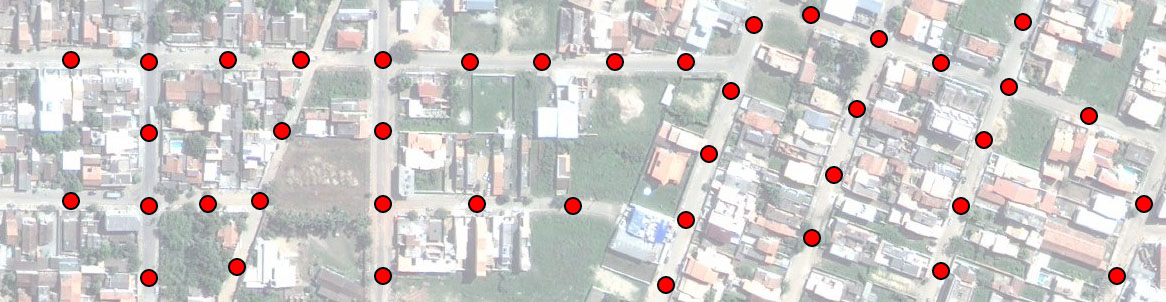
\includegraphics[width=0.98\textwidth]{figs/seeding.jpg}}
    \caption{Exemplo de uma semea��o �tima sobre uma imagem �ptica.}    
    \label{figuraSeeding1}   
\end{figure}

Geralmente, esse tipo de resultado � obtido a partir de m�todos robustos de semea��o. Na imagem acima, por exemplo, a identifica��o destas estradas possivelmente necessitaria de recursos computacionais na qual consideraria a largura do objeto a ser identificado, seus valores espectrais, sua curvatura, varia��o da intensidade de cores, os poss�veis obst�culos (como �rvores, carros e edifica��es), inclina��o, bifurca��es, entre outras.
Considerar todas essas caracter�sticas nem sempre � uma tarefa f�cil, ainda sim, alguns pontos n�o s�o devidamente marcados ou s�o marcados incorretamente, fazendo com que o m�todo sempre chegue a resultados bons, mas n�o �timos. Em imagens �pticas, a acur�cia dos resultados � uma quest�o relativamente f�cil de se alcan�ar, quando comparada � de imagens de radar. Nessas imagens a redu��o do ru�do \emph{speckle} (ru�do inerente de imagens de radar) � quase sempre uma etapa necess�ria de pr�-processamento.

Uma vez que a semea��o seja aplicada, a informa��o das prov�veis localiza��es das estradas torna-se conhecida, assim, o processo de extra��o torna-se ainda mais r�pido e eficiente, justificando assim, a import�ncia da semea��o no processo. \citeonline{harvey} destaca a import�ncia da qualidade dos pontos iniciais para o desempenho do algoritmo de extra��o. Geralmente, o m�todo de semea��o � utilizado em alguns trabalhos como predecessor ao algoritmo de extra��o. Algoritmos como o delineador de estradas (\emph{road trackers}) e Modelo de Contorno Ativo (\emph{Snakes}) s�o exemplos de m�todos de extra��o que utilizam a marca��o de pontos-sementes.

Na literatura, a semea��o na abordagem de extra��o de estradas pode ser categorizada em autom�tica, semiautom�tica e manual. Alguns dos trabalhos s�o descritos a seguir. 

\subsection{Semea��o Autom�tica}
A semea��o autom�tica � realizada sem nenhuma interfer�ncia humana, ou seja, tanto a defini��o dos par�metros do m�todo quanto a sua aplica��o � realizada de forma aut�noma. 

\citeonline{hu} utilizaram o conceito para o delineamento de estradas sobre imagens �pticas, onde a semea��o � realizada de forma autom�tica. Os autores pr�-estabelecem as geometrias ideais de uma estrada, definindo formas diferentes para as vias, tais como vias com interse��es e cont�nuas. A partir destas, � realizada uma varredura na imagem, buscando os pontos em que a correla��o com essas formas s�o menores que um determinado limiar.

\citeonline{pete2} propuseram um eficiente m�todo para a identifica��o do eixo de simetria de estradas em imagens �pticas. A abordagem apresentada identifica as bordas paralelas das estradas de acordo com um operador gradiente, que a partir do \emph{pixel} central da via, fornece tanto a orienta��o da borda quanto a sua localiza��o. Tal processo � realizado pelo algoritmo denominado extrator de eixo anti-paralelo (\emph{Anti-parallel Centerline Extractor - ACE}), proposto em \citeonline{agouris2}. Ap�s a identifica��o das bordas, o processo � seguido pela constru��o da rede de estradas com o aux�lio do algoritmo de auto-organiz�vel de mapeamento de estradas (\emph{Self-Organizing Road Mapping - SORM}), proposto em \citeonline{pete2}.

% zlotnick a. and carmine, p. 1993. Finding road seeds in aerial images. Computer Vision, graphics, and image processing: image 
% understanding 57.

\subsection{Semea��o Semiautom�tica}
Este processo, realizado de forma semiautom�tica, diferencia-se apenas pela interfer�ncia humana em parte do processo. Essa interfer�ncia pode ocorrer no in�cio do m�todo (por exemplo marca��o de ponto inicial ou de partida), ou no final (por exemplo ajuste na dire��o durante o delineamento). 

\citeonline{zhao} apresentaram um algoritmo semiautom�tico para a extra��o de estradas em imagens �pticas orbitais de alta resolu��o. A metodologia apresentada consiste em tr�s etapas, na qual a imagem � submetida a um processo de classifica��o em uma primeira etapa, e, por meio das classes identificadas como rodovias, � definida uma m�scara para utiliza��o nas etapas posteriores. A segunda etapa � caracterizada pelo processo de semea��o. Nesta, � obtido primeiramente uma imagem bin�ria correspondente �s bordas da imagem. Os pontos s�o marcados, conforme a an�lise dos vizinhos dos \emph{pixels} de borda. Na terceira e �ltima etapa da extra��o, � realizado um processo iterativo, em que, em cada itera��o, um modelo de estrada retangular � rotacionado sobre o eixo dos pontos, de forma que a dire��o do novo ponto apresente maior correla��o entre todas as dire��es analisadas. A rota��o da estrada sobre o eixo dos pontos � ilustrada na Figura \ref{seedingRotatinga}. Este m�todo � considerado uma abordagem semiautom�tica, pois a cada nova dire��o processada pelo m�todo, esta pode ser contestada e remarcada pelo operador, caso desej�vel.
\begin{figure}[htb]
    \centering    
    \subfigure{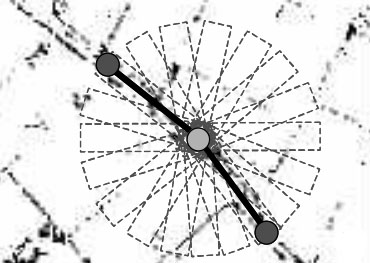
\includegraphics[width=0.36\textwidth]{figs/seeding2.jpg}}
    \caption{Rota��o de estrada retangular sobre o eixo dos pontos num processo de Semea��o semiautom�tica.}    
    \FONTE{Adaptado de \citeonline{zhao}.}
    \label{seedingRotatinga}   
\end{figure}

%merlet, n. and zerubia, J. 1996. New prospects in line detection by dynamic programming. ieee transactions on pattern analysis and machine
% intelligence 18(4), pp. 426-431.

\subsection{Semea��o Manual}
Neste tipo de semea��o, todos os pontos s�o marcados por um operador humano. \citeonline{dalpoz} utilizaram o conceito de programa��o din�mica para a extra��o de rodovias em imagens �pticas aerotransportadas e orbitais. O processo � inicializado por um operador humano, que fornece, grosseiramente, pontos sementes descrevendo a regi�o da estrada. 

\citeonline{fazan2} apresentam um m�todo de extra��o de estradas com o aux�lio da semea��o manual de pontos. Nesta semea��o um operador define um conjunto de pontos-sementes, no qual o primeiro identifica o in�cio da rodovia, e um segundo a dire��o. O processo de extra��o � realizado pelo delineamento da estrada por estrat�gia de teste ativo, t�cnica relacionada com o conceito de vis�o ativa \cite{dalpoz2}, que analisa a trajet�ria local do �ltimo ponto extra�do, resultando, por fim, no eixo central da via.

\citeonline{gruen2} utilizaram tamb�m um semeador manual para a extra��o de estradas em imagens �pticas. Nesse trabalho, os autores apresentam uma nova abordagem para a extra��o de estradas, denominado como Linha Curvil�nea B�sica de M�nimos Quadrados ou \emph{LSB-Snakes} (\emph{Least Square B-spline Snakes}), que utiliza o ajuste dos m�nimos quadrados combinados ao m�todo \emph{Snakes} para o delineamento das fronteiras das vias.

Com essas diversas abordagens, conclui-se que a forma de se identificar a passagem de uma estrada em um determinado ponto na imagem pode ser obtida de diversas formas. A semea��o manual mostrou-se como a op��o mais vantajosa para o m�todo de extra��o. Com este tipo de semea��o, a localiza��o dos pontos se torna prop�cia � convers�o, uma vez que � poss�vel contornar obst�culos imprevistos na imagem, tais como �rvores ou nuvens, no caso de imagem �ptica, e estradas com ru�do, no caso de imagens de radar. Esse tipo de opera��o faz com que o processo tenha um prov�vel �xito, no entanto, exige ainda um operador humano. 

\section{Principais M�todos para a Extra��o de Estradas} 
\subsection{Classifica��o}
O processo de classifica��o consiste em categorizar os dados presentes nas imagens em diferentes classes de padr�es, de forma que seja atribu�da uma identidade ou valores de probabilidade para os dados analisados. Tais classes representam as fei��es e alvos terrestres, tais como: �gua, cerrado, �rea urbana, �rea de desmatamento, entre outras. A classifica��o nada mais � que o reconhecimento desses grupos, cujos membros exibem caracter�sticas comuns. 

A classifica��o de imagens pode ainda ser subdividida em supervisionada e n�o supervisionada. Na primeira, � definido um conjunto de amostras das categorias a serem utilizadas na classifica��o e, posteriormente, com o recurso computacional, processa a imagem de modo que cada regi�o analisada seja associada a uma das classes. A segunda � �til quando n�o se possui informa��es relativas �s classes de interesse na �rea imageada. Segundo \citeonline{haupt}, os classificadores podem ser utilizados para categorizar qualquer tipo de dados, o que implica que podem ser utilizados em n�veis diferentes no processo de extra��o de estradas, seja no pr�-processamento, processamento ou p�s-processamento. Na identifica��o de estradas, um classificador � tipicamente utilizado de acordo com as propriedades da estrada presente na imagem. Para o problema de extra��o de estradas em imagens digitais, \citeonline{haupt} categoriza cinco classificadores �pticos
 e supervisionados em:
\begin{itemize}
 \item Classificadores Espectrais: Os classificadores espectrais s�o utilizados para comparar a assinatura espectral da classe padr�o com as amostras n�o conhecidas. Existem diversas maneiras de se aplicar esse tipo de classificador, entre essas, as mais utilizadas s�o os classificadores estat�sticos, classificadores por Redes Neurais Artificiais (RNA) e classificadores \emph{fuzzy}\footnote{M�todo matem�tico
 (computacional) utilizado no tratamento de incertezas.}. 
 \item Classificadores Texturais: Os classificadores texturais visam dividir as classes de padr�es pelas propriedades texturais contidas na imagem. O processo de classifica��o se inicia definindo as classes de padr�es que ser�o utilizadas para a classifica��o dos mesmos.
 \item Classificadores Geom�tricos: Nesse tipo de classifica��o, as fei��es s�o identificadas por suas propriedades estruturais ou geom�tricas, ou seja, no caso da identifica��o de estradas, por exemplo, as fei��es tendem a aparecer na imagem como segmentos retos, cont�nuos, com largura relativamente pequena. Desta forma, estas informa��es estruturais s�o levadas em conta na defini��o das classes de padr�es que ser�o utilizadas na  classifica��o.
 \item Classificadores Contextuais: Na classifica��o contextual, � necess�rio que se conhe�am as informa��es dos \emph{pixels} vizinhos para  o desenvolvimento do processo de extra��o. A informa��o contextual, como � chamada, permite definir regi�es onde as estradas possuem caracter�sticas similares, tais como curvatura, largura e n�veis de intensidade. Sendo assim, � poss�vel otimizar o processo de extra��o em diferentes regi�es da imagem, a exemplo de estradas presentes em �reas urbanas, que podem diferenciar-se muito das estradas presentes em uma �rea de vegeta��o. 
 \item Classificadores por Padr�es Autom�ticos de Classes: Os classificadores por reconhecimento autom�tico de classe s�o classificadores que requerem algum m�todo de aprendizagem no seu processamento. A classifica��o por reconhecimento de padr�es consiste em armazenar as informa��es obtidas da leitura das classes de amostras, de forma que esta leitura seja �til em futuras identifica��es, ou seja, � constru�do uma base de conhecimento tal que ao apresentar um determinado padr�o a esse classificador, ele, por meio da correla��o entre seu conhecimento e dessa amostra, saber� dizer em qual classe esta pertencer�.
\end{itemize}

\citeonline{pete3} utilizaram o m�todo K-m�dias e os Mapas Auto-Organiz�veis para a classifica��o de imagens �pticas em alta resolu��o. O algoritmo intitulado SORM (\emph{Self-Organizing Road Map}), possibilita a conex�o dos pontos provenientes da classifica��o, de forma que seja aplicada uma an�lise topol�gica com m�tricas \emph{fuzzy}, obtendo-se, com isso, os eixos centrais do conjunto de estradas. 

\citeonline{baumgartner3} fazem um comparativo dos modelos de estradas reais com os presentes em imagens digitais e apresentam um classificador contextual para a extra��o de estradas. Ao considerar as caracter�sticas radiom�tricas, geom�tricas e topol�gicas de estradas, os autores definem as rela��es que estas estruturas podem ter com outros objetos na imagem, tais como �rvores, carros, edif�cios, entre outros. Tal rela��o � considerada como contexto local enquanto que, as informa��es quanto � regi�o em que a estrada se encontra, tal como floresta ou �rea urbana, s�o consideradas como contexto global. 

\citeonline{mena} apresentaram um m�todo autom�tico para a extra��o de estradas em imagens �ticas de alta resolu��o, abordando o uso de classificadores estat�sticos, em que o processo de classifica��o resulta em duas classes de padr�es, i.e., uma imagem bin�ria contendo as informa��es de estradas e n�o estradas. \citeonline{haralick} apresenta as diferentes abordagens de textura em uma imagem digital, e al�m disso, generaliza a abordagem estrutural-estat�stica para textura, agregando a este modelo, novas primitivas de texturiza��o.

\subsection{Transformada de Hough}
A Transformada de Hough (TH) � um operador matem�tico capaz de detectar formas geom�tricas em imagens digitais, tais como retas, c�rculos e elipses. Desenvolvida em 1962 por Paul Hough, tornou-se uma contribui��o relevante na �rea de vis�o computacional. O m�todo consiste em aplicar na imagem original uma transforma��o, tal que todos os pontos pertencentes a um mesmo segmento de reta sejam mapeados em um �nico ponto no dom�nio da TH. 

% Embora o m�todo seja aplic�vel em qualquer composi��o de imagem, ele � comumente aplicado sobre uma imagem bin�ria, geralmente ap�s o processamento de detectores de bordas. A transforma��o para o dom�nio da TH � expressa por:
% \begin{align}
% \rho = x~cos \theta + y~sen, \theta
% \end{align}
% em que $\rho$ representa a dist�ncia entre um determinado ponto da reta e a origem no plano-$xy$ (reta imagin�ria) e, $\theta$ � o �ngulo 
% entre o eixo $y$ e a reta imagin�ria. Na Figura \ref{figura1} � ilustrado como a transforma��o ocorre, tal que cada ponto no plano-$xy$ � 
% convertido em uma sen�ide no plano da TH, e desta forma, o segmento reto presente na imagem poder� ser interpretado pelos m�ximos presentes 
% no dom�nio da TH, ou seja, nas interse��es das sen�ides de cada ponto da reta.
% \begin{figure}[htb]
%     \centering
%     \subfigure[]{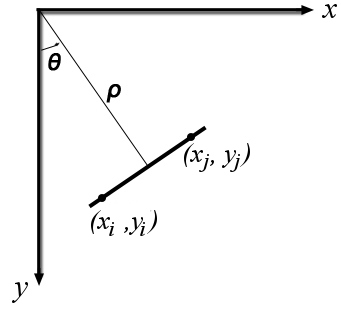
\includegraphics[width=0.33\textwidth]{figs/th_graf3.jpg}} \hspace{0.3cm}
%     \subfigure[]{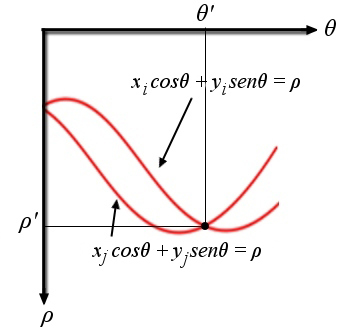
\includegraphics[width=0.33\textwidth]{figs/th_graf2.jpg}}
%     \caption{Parametriza��o de ($\rho$, $\theta$): (a) No plano-$xy$ (imagem). (b) No dom�nio da TH.}
%     \FONTE{Adaptado de \citeonline{woods}.}
%     \label{figura1}   
% \end{figure}

Por ser um operador muito eficiente na detec��o de linhas, a TH � muito utilizada na extra��o de fei��es lineares. \citeonline{gamba4} apresentaram uma varia��o do algoritmo, de forma a serem consideradas diferentes larguras para as fei��es. Al�m de reduzir o tempo de processamento, o algoritmo fornece melhores resultados, detectando os pontos de in�cio e t�rmino dos segmentos retos, ao inv�s de linhas completas. A utiliza��o da TH pode ser aplicada tamb�m na detec��o de curvas com baixo grau de curvatura. 

\citeonline{amberg} utilizaram, a princ�pio, a Programa��o Din�mica para a extra��o dos eixos centrais das vias, e posteriormente, a TH � utilizada para a conex�o dos pontos descont�nuos provenientes da extra��o. 

\citeonline{hu2} obtiveram bons resultados utilizando a TH como auxiliadora no processo de extra��o de estradas. O m�todo apresentado pelos autores � usado em uma imagem �ptica de alta resolu��o, em que a TH � aplicada iterativamente sobre uma imagem classificada, at� que se obtenham todas as vias. 

\subsection{Morfologia Matem�tica}
A morfologia matem�tica � utilizada h� muito tempo no processamento de imagens digitais, e as aplica��es realizadas com operadores morfol�gicos remetem � Teoria dos Conjuntos. Processos como uni�o, interse��o, dilata��o, eros�o, fechamento, abertura e afinamento s�o opera��es fundamentais na morfologia matem�tica. Os operadores s�o utilizados no problema de extra��o de estradas para a remo��o de pequenas regi�es indesej�veis, tais como buracos, sombras ou carros, permitindo tamb�m a suaviza��o de formas e contornos. Na extra��o de estradas, a morfologia matem�tica � frequentemente utilizada como filtro durante as etapas de pr� e p�s-processamento \cite{haupt}. 

Os processos de dilata��o, eros�o, abertura e afinamento formam a base da morfologia matem�tica \cite{woods}. Tais t�cnicas s�o frequentemente utilizadas como recurso na extra��o de estradas. \citeonline{chanussot} apresentaram um m�todo autom�tico para a extra��o de fei��es lineares em imagens \emph{SAR}, na qual utilizaram operadores morfol�gicos para a filtragem das estradas e remo��o de regi�es indesej�veis. A princ�pio, s�o definidos as caracter�sticas geom�tricas da via, tais como largura, contraste e comprimento. Na Figura \ref{figOpMorfologicos3} � ilustrado este processo em um recorte na imagem. Para tais filtragens, os autores utilizaram o operador morfol�gico de abertura (\emph{opening}) para a remo��o de pequenas regi�es escuras e entorno claro, denominados vales Figura \ref{morf0b}, em seguida � aplicado o mesmo operador, no entanto, direcional, removendo cristas descont�nuas Figura \ref{morf1}. Ap�s a remo��o desses pontos, a imagem torna-se mais suave, aplicando-se o operador de fechamento (\emph{closing}) as regi�es de vales s�o removidas Figura \ref{morf2}. Por fim, � aplicado o operador cartola (\emph{top-hat}) para a remo��o de res�duos escuros, restantes do �ltimo processamento, resultado em uma imagem com fei��es claras real�adas Figura \ref{morf3}.
\begin{figure}[htb]
    \centering
    \subfigure[]{\label{morf0a}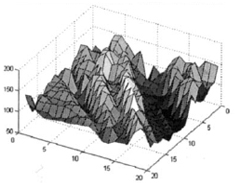
\includegraphics[width=0.32\textwidth]{figs/morf0a.jpg}} \hspace{0.5cm}
    \subfigure[]{\label{morf0b}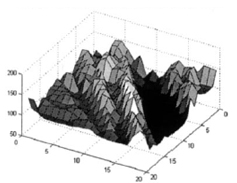
\includegraphics[width=0.32\textwidth]{figs/morf0b.jpg}} \\
    \subfigure[]{\label{morf1}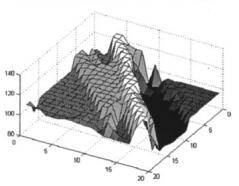
\includegraphics[width=0.32\textwidth]{figs/morfol1a.jpg}} 
    \subfigure[]{\label{morf2}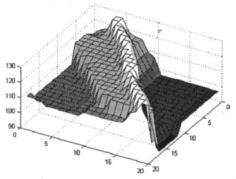
\includegraphics[width=0.32\textwidth]{figs/morfol2a.jpg}} 
    \subfigure[]{\label{morf3}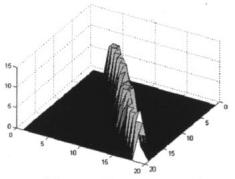
\includegraphics[width=0.32\textwidth]{figs/morfol3a.jpg}}   
    \caption{Aplica��o do operador morfol�gico de abertura para realce de estradas. (a) Imagem original. (b) Imagem ap�s a aplica��o do 
    operador de abertura. (c) Imagem ap�s a aplica��o do operador de abertura direcional. (d) Imagem ap�s a aplica��o do operador de fechamento. 
    (e) Imagem final, ap�s a aplica��o do operador \emph{top-hat}.} 
    \FONTE{Adaptado de \citeonline{chanussot}.}
    \label{figOpMorfologicos3}   
\end{figure}

\citeonline{idbraim} utilizaram o operador morfol�gico de abertura para a reconstru��o de elementos lineares em imagens �pticas. A opera��o � realizada com um operador direcional de estrutura linear, sendo sua largura de cinco \emph{pixels}. Esse processo � realizado em complemento na aplica��o de filtros de realces, onde s�o destacadas as fei��es conforme sua orienta��o. Um operador muito utilizado para a obten��o do eixo de simetria de fei��es lineares, � o operador de afinamento, que tem como objetivo obter o esqueleto da forma. 

\citeonline{zhang2} utilizaram o processo de afinamento para a obten��o dos eixos de simetria e estradas. O processo � realizado sobre uma imagem segmentada, onde s�o aplicados dois outros operadores: de abertura, para que sejam removidos pontos esp�rios da detec��o, e de fechamento, para que os extremos dos segmentos de estrada desconectados sejam conectados.

Os operadores morfol�gicos s�o, em geral, componentes importantes no processamento de imagens digitais e principalmente na extra��o de estradas. Sua aplica��o � eficaz na remo��o de regi�es indesejadas e opera��es que envolvam o contexto local. 

\subsection{Segmenta��o} 
O processo de segmenta��o por regi�es em imagens digitais � o processo de agrupamento de dadas regi�es, com o objetivo de simplificar a representa��o da imagem e, consequentemente, facilitar o seu processo e an�lise. \citeonline{barrow} definem como segmenta��o por regi�es o processo de particionamento de uma imagem em regi�es semanticamente interpretadas. O resultado gerado a partir deste processo consiste em um conjunto de regi�es disjuntas, com interse��o nula e cuja uni�o do conjunto de regi�es � a pr�pria imagem, ou seja, considerando $I$ uma imagem, a segmenta��o � o processo que particiona $I$ em $n$ sub-regi�es $R_i$, para $i=1,2,...,n$, tal que:
\begin{enumerate}
 \item $\cup_{i=1}^n R_i = I$       
 \item $R_i$ � uma regi�o conectada, $ i=1,2,...,n$
 \item $R_i \cap R_j = \varnothing ~ \forall ~ i\neq j$
 \item $P(R_i) = $ verdadeiro, $ i=1,2,...,n$
 \item $P(R_i \cup R_j) = $ falso, para $ i\neq j$
\end{enumerate}
em que $P(R_i)$ representa um predicado l�gico sobre os pontos no conjunto $R_i$. A primeira condi��o indica que todos os \emph{pixels} da imagem pertencem a uma determinada regi�o. A condi��o \textbf{b} indica que todos os pontos de uma determinada regi�o devem estar conectados. A condi��o \textbf{c} indica que as regi�es devem ser disjuntas. A condi��o \textbf{d} determina a propriedade que deve ser satisfeita pelos \emph{pixels} em uma determinada sub-regi�o. Por �ltimo, a condi��o \textbf{e} indica que as sub-regi�es $R_i$ e $R_j$ s�o distintas em rela��o � propriedade definida \cite{woods}. Os \emph{pixels} pertencentes a uma dada regi�o possuem caracter�sticas similares, e cada regi�o difere significativamente de suas vizinhas.

Assim como a semea��o, a segmenta��o n�o � considerada um m�todo de extra��o de estradas como listado nessa se��o, embora seja uma opera��o muito �til e eficiente em grande parte dos m�todos de extra��o. O resultado desta opera��o permite separar as diversas regi�es contidas na imagem em regi�es �nicas e bem definidas, tornando poss�vel, por exemplo, a sele��o dos segmentos pertencentes �s regi�es de estradas. A segmenta��o tem um papel importante no processamento de imagens de radar. \citeonline{mena} utilizaram a segmenta��o baseada na an�lise de textura da imagem, em que o processo � realizado sobre uma imagem �ptica. Ap�s concluir a etapa de segmenta��o, a imagem � submetida a um processo de esqueletoniza��o, fornecendo os eixos de simetria da rede de estradas. \citeonline{amini2} utilizaram o m�todo de divis�o e jun��o (\emph{split and merge}) para a segmenta��o. O m�todo � baseado na estrutura \textquotedblleft \emph{quadtree}\footnote{�rvore estrutural de dados em que subdivide recursivamente a imagem em quadrantes de quatro, a fim de determinar a homogeneidade de regi�es \cite{finkel}.}\textquotedblright$~$para a parti��o da imagem, que explora as regi�es homogenias (\emph{split}) e em seguida as combinam caso suas vizinhas possuir caracter�sticas semelhante. Ao fim, � criada uma imagem segmentada. 

\citeonline{grote} utilizaram o conceito de segmenta��o para a extra��o de estradas em imagens �pticas de alta resolu��o, focando a extra��o em �reas urbanas. Com o processo de segmenta��o, s�o geradas pequenas regi�es na imagem cujas bordas coincidem com as bordas das estradas, e os extremos de cada regi�o s�o ent�o conectados aos extremos de outras regi�es, de acordo com crit�rios de dist�ncia, dire��o e �ngulo.

\subsection{Modelos Deform�veis}
O conceito tradicional denominado Modelo de Contorno Ativo ou simplesmente \emph{Snakes}, possui um grande n�mero de trabalhos abordando-o como m�todo extrator de estradas, principalmente, ao se tratar da obten��o dos eixos centrais das vias. Desenvolvido inicialmente por \citeonline{kass}), o m�todo consiste em um processo iterativo e adaptativo para a identifica��o de contornos de objetos, de modo que uma 
curva poligonal seja convergida para as formas do objeto. O progresso da curva at� a localiza��o desejada � alcan�ada minimizando-se, a cada ciclo iterativo, uma determinada propriedade da curva, denominada energia. A Figura \ref{figSnake} ilustra este processo em sua representa��o tradicional.
\begin{figure}[htb]
    \centering
    \subfigure[]{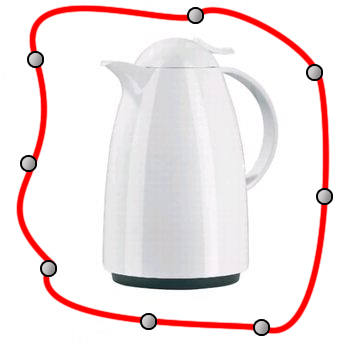
\includegraphics[width=0.30\textwidth]{figs/snake3.jpg}} \hspace{0.3cm}   
    \subfigure[]{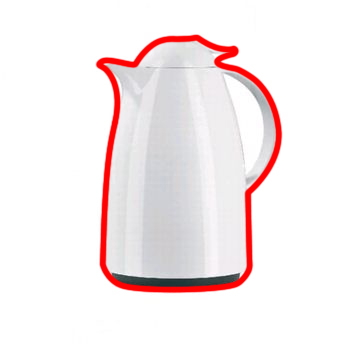
\includegraphics[width=0.30\textwidth]{figs/snake4.jpg}}   
    \caption{Ilustra��o da aplica��o de \emph{Snakes} com curva fechada (m�todo tradicional) para a identifica��o de objetos: (a) Interpola��o 
    inicial. (b) Evolu��o final da curva.}
    \label{figSnake}   
\end{figure}

A utiliza��o de Modelos Deform�veis na extra��o de estradas em imagens digitais consiste em uma abordagem promissora, embora se trate de uma t�cnica complexa, sua utiliza��o permite identificar com exatid�o o contorno de objetos presentes na cena. No entanto, o modelo apresenta uma sensibilidade muito grande quanto a sele��o de seus par�metros. Na literatura, os trabalhos de extra��o de estradas abordando o uso de Modelos Deform�veis mostram-se eficazes em imagens �pticas. Por outro lado, na imagem de radar, a aplica��o desse modelo possui limita��es, justamente pela presen�a de ru�do em grande quantidade. A �rea de Modelos Deform�veis possui in�meras variantes, todas com o objetivo de reconhecer o contorno de objetos presentes na cena. Nesta se��o, ser�o apresentados alguns trabalhos que utilizaram tal recurso para a extra��o de estradas, destacando, principalmente, o Modelo de Contorno Ativo, que ser� melhor discutido na Se��o \ref{snakes}.

\citeonline{silvestre} introduz algumas das t�cnicas para a obten��o de contornos de objetos, tais como o Modelo Geom�trico (\emph{Level Set}) \cite{osher}, cujo processo de identifica��o de contornos n�o necessita da parametriza��o da curva, embora basear-se tamb�m na otimiza��o de uma fun��o objetivo. O Modelo de Formas Ativas (\emph{Active Shape Models}) \cite{cootes} n�o � uma abordagem param�trica, ao inv�s disso, 
o modelo se baseia nas caracter�sticas do objeto a ser identificado, que ap�s definido, aplica-se o processo de deforma��o, obtendo o contorno das formas de acordo com a minimiza��o da dist�ncia entre os pontos correspondentes � forma e ao objeto a ser extra�do. Os Modelos Probabil�sticos \cite{staib} permitem incorporar fun��es de probabilidade tal que delimitem na imagem, as estruturas das classes a serem extra�das. 

Outros m�todos, como o modelo Bal�o (\emph{Balloon})\cite{cohen}, possui caracter�sticas semelhantes comparado ao m�todo tradicional, no entanto, a curva inicial deste � iniciada dentro do objeto a ser extra�do, e evolui at� que se alcance as fronteiras do objeto, comportando-se como um bal�o ao ser enchido. O m�todo de Fluxo do Vetor Gradiente (\emph{Gradient Vector Flow - GVF}) \cite{xu} � uma outra alternativa para a aquisi��o de 
contornos de objetos. Trata-se tamb�m de uma abordagem param�trica que agrega uma nova energia externa baseando-se no gradiente da imagem. O conceito apresenta benef�cios, principalmente, pela n�o necessidade de pontos-sementes pr�ximos ao contorno, al�m de convergir eficientemente para as formas do objeto. 



O m�todo possibilitou uma significante contribui��o para a �rea de Vis�o Computacional. Como mencionado anteriormente, surgiram in�meras variantes a partir desse trabalho, entre essas evolu��es, o m�todo \emph{Snakes} deixou de ser modelado apenas como uma curva fechada, como em sua representa��o original, mas passou tamb�m a possuir representa��es abertas. A curva aberta possibilita o delineamento de segmentos retos, tais como as estradas na Figura \ref{figSnake1}. 
\begin{figure}[htb]
    \centering
    \subfigure[]{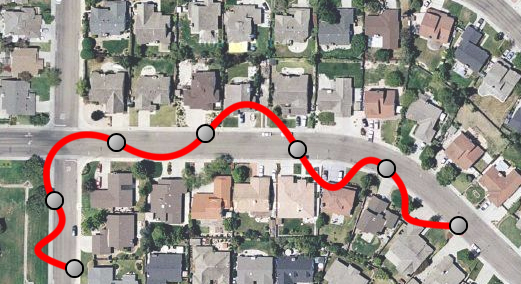
\includegraphics[width=0.48\textwidth]{figs/snake1.jpg}} \hspace{0.1cm}   
    \subfigure[]{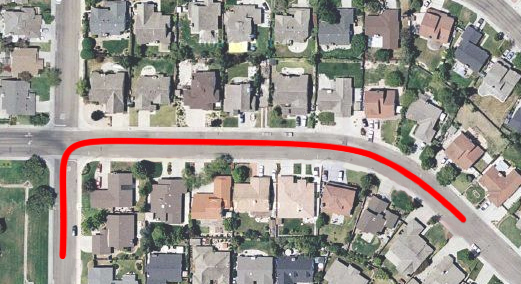
\includegraphics[width=0.48\textwidth]{figs/snake2.jpg}}   
    \caption{Ilustra��o da aplica��o de \emph{Snakes} com curva aberta para a identifica��o de estradas: (a) Interpola��o inicial. (b) Evolu��o 
    final da curva em um processo de obten��o do eixo de simetria.}
    \label{figSnake1}   
\end{figure}

Dada as suas caracter�sticas o m�todo \emph{Snakes} � frequentemente utilizado na extra��o de estradas. \citeonline{gruen} utilizaram uma extens�o ao m�todo, cuja abordagem permite extrair os eixos centrais das vias em imagens �pticas. Nessa abordagem, o m�todo \emph{Snakes} � executado em conjunto com a Programa��o Din�mica \cite{bellman2}, o qual � utilizada como m�todo de otimiza��o na evolu��o da curva. A abordagem apresentada pelos autores permite a extra��o de estradas, nas quais existam obst�culos, como sombras causadas por �rvores, ve�culos, edifica��es. 

\citeonline{mayer} utilizaram o m�todo \emph{Ribbon-Snakes} em imagens �pticas de alta resolu��o. O m�todo estende a abordagem tradicional de \emph{Snakes}, em que acrescenta uma caracter�sticas de largura $w$ no modelo param�trico. Desta forma, ao extrair o eixo de simetria da fei��o de interesse, s�o expandidos paralelamente ao ponto $(x_i,y_i)$, a dist�ncia $w_i$ para cada um dos lados da curva, de modo a obter as fronteiras das estradas Figura \ref{figribbonsnake}. Em rela��o a abordagem tradicional, o m�todo \emph{Ribbon-Snakes} pode apresentar algumas vantagens. Obter as bordas da estrada � um processo �til em regi�es em que a largura das vias varia ou, at� mesmo, por se obter a largura das vias mesmo em condi��es adversas, tal como a presen�a de sombras ou �rvores (em imagens �pticas) que prejudicam a identifica��o real das fronteiras. O mesmo � considerado para a imagem de radar, embora os obst�culos na extra��o sejam outros.
\begin{figure}[htb]
    \centering
    \subfigure{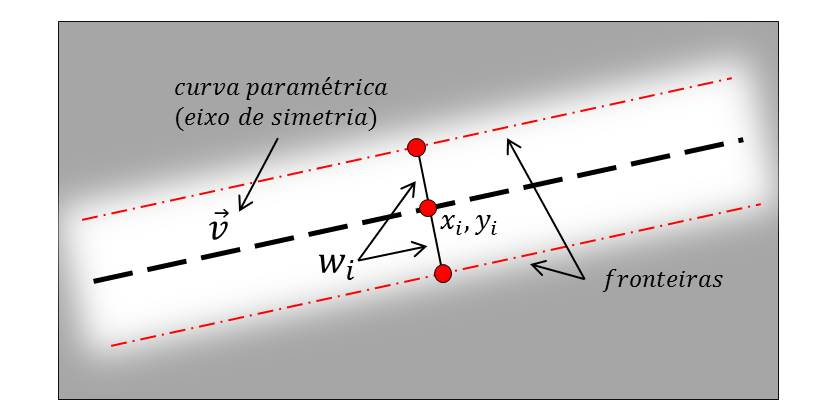
\includegraphics[width=0.66\textwidth]{figs/ribbonsnakes.jpg}}      
    \caption{Ilustra��o do conceito de expans�o do m�todo \emph{Ribbon-Snakes}.}
    \FONTE{Adaptado de \citeonline{mayer}.}
    \label{figribbonsnake}   
\end{figure}

\citeonline{bentabet} propuseram um m�todo para a extra��o de estradas em imagens de radar, utilizando para tanto o m�todo \emph{Snakes}. Em uma etapa de pr�-processamento, os autores utilizaram filtros redutores de ru�do \emph{speckle}, destacando os filtros de \emph{Frost}\cite{frost} e \emph{Lee}\cite{lee} como sendo filtros eficientes na minimiza��o deste tipo de ru�do. Ap�s a etapa de suaviza��o, � aplicado um detector de linhas, proposto por \citeonline{ziou} e, por fim, utilizou-se de \emph{Snakes} para a extra��o das vias. Os par�metros de rigidez e elasticidade (ver Se��o \ref{snakes}), utilizados pela \emph{Snakes}, s�o estimados automaticamente no processo de extra��o apresentado. 

\citeonline{agouris} apresentaram  uma extens�o do m�todo \emph{Snakes} para a detec��o de estradas em imagens �pticas, denominado Modelo de \emph{Snakes} diferencial. Neste caso, o m�todo original � acrescido de um novo termo, que � relacionado com as informa��es da imagem existentes em um banco de dados geogr�ficos. Tal termo descreve a diferen�a entre a solu��o atual da curva com a informa��o pr�-existente. Com isso, s�o analisadas as mudan�as geoespaciais das estradas em rela��o ao dado armazenado e, se houver mudan�as consider�veis, estas s�o atualizadas no banco.

\citeonline{bentabet} classificaram os principais trabalhos envolvendo a extra��o de estradas em imagens de radar, organizando-os por complexidade. Na pr�xima se��o, s�o apresentados alguns desses trabalhos, que n�o se enquadraram de forma espec�fica nos t�picos apresentados neste cap�tulo, por�m, possuem grande import�ncia na literatura sobre a extra��o de estradas em imagens digitais.

\subsection{Outras Abordagens}
Muitos dos trabalhos envolvendo o problema de extra��o de estradas, n�o possuem ainda uma abordagem espec�fica para a sua resolu��o, alguns por apresentarem conceitos h�bridos, outros por apresentarem conceitos inovadores. Nesta se��o, s�o descritos alguns dos importantes trabalhos envolvendo a extra��o de estradas em imagens de radar.

\citeonline{tupin} propuseram um eficiente m�todo autom�tico para a extra��o de fei��es lineares em imagens de radar. Para tanto, os autores dividiram o processamento em duas etapas. A primeira � caracterizada pela detec��o das estruturas lineares na imagem, onde s�o utilizados dois filtros: o detector de bordas por rela��o \cite{bovik}, utilizado para o realce de linhas na presen�a de ru�do \emph{speckle}, e um segundo filtro proposto pelos autores, que consiste em um detector de linhas por correla��o cruzada, chamados pelos autores de D1 e D2, respectivamente. Os resultados de ambos detectores s�o combinados e repassados � segunda etapa do processamento, esta caracterizada pela conex�o dos segmentos lineares e constru��o da rede de estradas. Isso � executado, criando-se um Campo Aleat�rio Markoviano (\emph{Markov Random Field - MRF}), t�cnica melhor fundamentada em \citeonline{spitzer}, em que, para cada extremo dos segmentos de reta, � agregada uma probabilidade de jun��o, probabilidade esta estabelecida de acordo com regras geom�tricas entre o par de pontos, indicando a poss�vel 
conex�o. Assim, � gerado um mapa de poss�veis conex�es, na qual somente os pares com probabilidades satisfeitas segundo um limiar s�o conectados. 

\citeonline{costa} estenderam a abordagem dos detectores de \citeonline{tupin} e aplicaram a TH sobre o resultado dos detectores proposto pelos autores. \citeonline{lisini2} utilizaram tamb�m os detectores propostos em \citeonline{tupin}. Nessa abordagem apresentada pelos autores, s�o aplicados os detectores de linhas e, posteriormente, ajusta-se os resultados com a imagem classificada. Com isso, � realizado um processo de reconstru��o da rede de estradas, na qual s�o selecionados os segmentos de reta que satisfazem os valores de largura (\emph{pixels}) e orienta��o. Selecionadas as vias, estas s�o submetidas ao operador morfol�gico de afinamento, que obt�m seus eixos de simetria. Finalmente, � aplicado um algoritmo de lineariza��o, tornando-as mais alinhadas.

\citeonline{zhou} combinaram a an�lise multiescala com informa��es polarim�tricas para a extra��o de fei��es lineares em imagens de radar. S�o aplicados detectores de linhas em baixa resolu��o em diferentes polariza��es da imagem. Em seguida, cada resultado � submetido a uma combina��o. Em uma segunda etapa, � realizada a detec��o de linhas em alta resolu��o, em que s�o aplicados detectores \emph{fuzzy} em uma imagem filtrada.

\citeonline{baumgartner2} propuseram um m�todo autom�tico para a extra��o de estradas em imagens �pticas, utilizando o conceito multiescala combinado � an�lise do contexto global e local da imagem. Inicialmente, o processo de extra��o � realizado sobre �reas rurais, e depois estendido �s �reas urbanas e de florestas. Esta ordem de processamento � justificada j� que nas �reas rurais possuem interfer�ncias menores de objetos como edif�cios, autom�veis ou �rvores, e assim, o processo realizado nas �reas rurais pode ser utilizado como modelo para as etapas seguintes. Esse processo � realizado em diferentes escalas da imagem, onde, em baixas resolu��es s�o aplicados filtros detectores de borda. A partir desta an�lise, s�o obtidas as hip�teses dos segmentos de estradas, os quais s�o posteriormente combinados, formando a rede de estradas. A abordagem se mostrou �til n�o s� pelo resultado da extra��o, mas tamb�m por apresentar efici�ncia nos resultados onde houve intersec��es de vias.

\citeonline{xiao} propuseram uma nova forma de extrair estradas em imagens de radar. A abordagem tratada pelos autores remete � Intelig�ncia Computacional, com o uso de algoritmo gen�tico (\emph{Genetic Algorithm - GA}). A princ�pio, a imagem � submetida a uma etapa de pr�-processamento, na qual � realizada a classifica��o da mesma em classes, como vegeta��o, �reas de constru��es e estradas. A classifica��o � realizada por um operador \emph{fuzzy}, denominado FCM (\emph{Fuzzy C Means}). Ap�s a classifica��o, � atribu�do um conjunto de pontos sementes para cada segmento de estrada, em que, para cada conjunto, � estabelecida uma curva passando por seus respectivos pontos. O GA implica na busca de solu��es inspirada na gen�tica humana de evolu��o.

Entre as in�meras t�cnicas para a extra��o de estradas tanto em imagens �ticas como de radar, nesta se��o foram destacadas as de maior import�ncia na literatura. O levantamento de solu��es para o problema � vasto, e fica evidente que outros m�todos adequariam-se perfeitamente ao conte�do deste trabalho. Um levantamento mais completo envolvendo a extra��o de estradas � apresentado por \citeonline{mena2}.

Grande parte dos trabalhos na �rea utilizam operadores manuais ou semiautom�ticos para a semea��o. Um m�todo completamente autom�tico, tal como apresentado por \citeonline{tupin}, � constru�do, geralmente, sobre muita pesquisa e cautela. Os detalhes envolvendo a implementa��o autom�tica s�o, quase sempre, constitu�dos por modelos complexos de extra��o de estradas, o que acaba por ultrapassar o escopo desta pesquisa. O prop�sito deste trabalho � apresentar um operador que realize a extra��o dos eixos de simetria das estradas e caminhos presentes em imagens de radar \emph{SAR} aerotransportadas, de forma que este processo seja realizado de maneira semiautomatica. Para tanto, ser� apresentada uma abordagem h�brida, utilizando dois conceitos descritos anteriormente: o m�todo de semea��o para a identifica��o de pontos que caracterizam a presen�a de uma estrada, conjugado ao m�todo \emph{Snakes}. 

O m�todo de semea��o apresentado � fundamentado em t�cnicas de Intelig�ncia Computacional, mais precisamente nos Mapas Auto-Organiz�veis, t�cnica que permite o reconhecimento de formas em imagens digitais, de acordo com padr�es de treinamento. O m�todo de semea��o possui autonomia em parte de sua execu��o, portanto, � denominado um m�todo semiautomatico. O pontos-sementes identificados pelo semeador s�o interpolados conforme o segmento
de reta identificado, a curva inicial gerada � aplicada ao m�todo \emph{Snakes} que, por fim, obt�m os eixos centrais das estradas. Este trabalho n�o busca uma solu��o �tima para o problema, mas sim a pesquisa acerca da utiliza��o de m�todos espec�ficos em processamento de imagem de radar de abertura sint�tica de alta resolu��o espacial.

% Para a an�lise e valida��o dos resultados obtidos, ser� utilizada a curva caracter�stica operacional de receptor (\emph{Receiver Operating Characteristic - ROC}) \cite{green}, que permite avaliar a rela��o dos pontos identificados corretamente ou verdadeiro positivo (\emph{true positive - TP}) e identificados incorretamente ou falso positivos (\emph{false positive - FP}). 

No cap�tulo seguinte, ser� apresentado o detalhamento do processo de extra��o de estradas. A primeira parte da se��o � destinada � apresenta��o dos dados utilizados para o conjunto de testes do m�todo. Na segunda parte, s�o descritos todas as etapas de desenvolvimento do m�todo, iniciando-se pelo detalhamento do m�todo de semea��o e, posteriormente, o m�todo \emph{Snakes} para a identifica��o de estradas. Por fim, os resultados s�o analisados e discutidos, seguindo crit�rios espec�ficos de avalia��o. 




 %% 2o capitulo
\chapter{CONCEITOS E TECNOLOGIA}\label{conceitosTec}
Neste cap�tulo, s�o apresentados conceitos envolvendo a implementa��o do m�todo de extra��o de estradas. A princ�pio, s�o apresentados os fundamentos do imageamento por radar, em que s�o mostrados os conceitos b�sicos envolvendo a aquisi��o de uma imagem SAR. Em seguida, s�o apresentadas as caracter�sticas matem�ticas da estrada, objeto a ser extra�do na imagem. Por fim, descreve-se o procedimento para a extra��o de estradas utilizando os m�todos de Semea��o e Modelo de Contorno Ativo.

\section{Fundamentos do imageamento por radar}
A geometria b�sica da forma��o de uma imagem \emph{SAR} aerotransportada pode ser ilustrada pela Figura \ref{figura2}, em que $V$ determina a velocidade segundo a qual a plataforma se move em uma determinada dire��o, conhecida tamb�m por dire��o de azimute. O par�metro $H$ representa a altitude em que ela se encontra. Esta plataforma transporta uma antena com observa��o lateral, que ilumina a superf�cie em estudo com pulsos de radia��o eletromagn�tica. A dist�ncia da plataforma at� a �rea iluminada � conhecida como \emph{slant range} $R_0$, e a dist�ncia da superf�cie da Terra sobre a qual se encontra a plataforma (nadir) at� a �rea iluminada � conhecida como \emph{ground range}, expresso por $R_g$ na Figura \ref{figura2} \cite{oliver}.
\begin{figure}[htb]
    \centering	   
    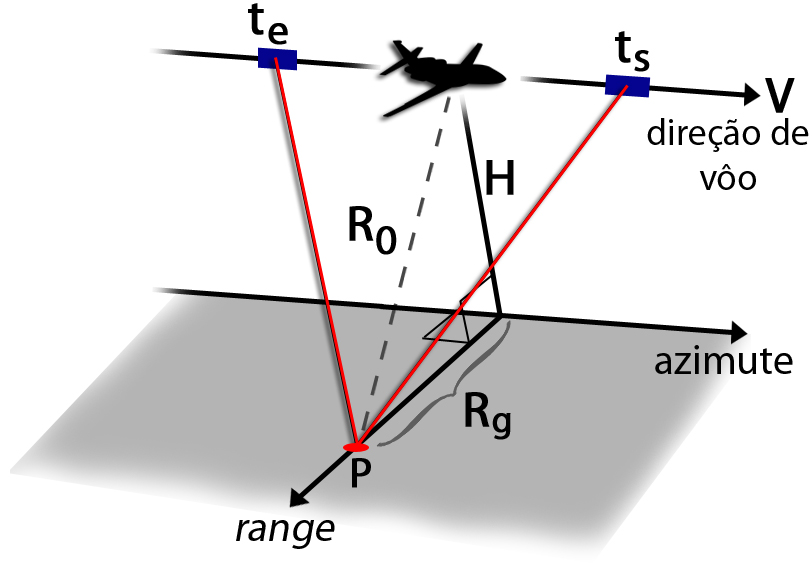
\includegraphics[width=0.53\textwidth]{figs/plane2.jpg}\\
    \caption{Geometria de imageamento de radares aerotransportados de visada lateral.}    
    \FONTE{Adaptado de Oliver e Quegan (\citeyear{oliver}).}
    \label{figura2}   
\end{figure}

Os sistemas de radar s�o formados por um transmissor, receptor, antena, processador de sinais e uma unidade de visualiza��o. Uma sequ�ncia de pulsos � emitida em intervalos de tempos regulares, sendo que esses sinais se propagam em uma �rea iluminada pela antena. O objeto iluminado absorve uma fra��o da energia incidente e espalha o restante de acordo com os par�metros do sistema e as propriedades f�sicas do objeto. Parte da energia espalhada � retornada para o sensor, caracterizando o sinal recebido \cite{carrara}.

Os sensores a bordo de aeronaves permitem obter imagens com maior resolu��o (1 a 20 metros) quando comparados aos sensores a bordo de sat�lites, por�m sua �rea iluminada � menor. Os sat�lites podem visualizar uma �rea maior da superf�cie da Terra. Estando continuamente em �rbita terrestre, � relativamente f�cil coletar imagens da mesma �rea de modo sistem�tico, a fim de monitorar mudan�as na biosfera.

As imagens de radar s�o geradas a partir da emiss�o de pulsos de largura $T_p$ em intervalos de $T$ segundos. Utilizando o modelo de ponto fixo $P$, mostrado na Figura \ref{figura2}, o sistema de imageamento \emph{SAR} possui um intervalo de tempo ($t_s - t_e$), onde $t_e$ representa o ponto onde � iniciado a transmiss�o dos pulsos pelo sensor, e $t_s$ o ponto final da transmiss�o. Neste intervalo, o radar envia $N$ pulsos e coleta $N$ pulsos resultantes do retorno do ponto $P$. As amostras recebidas s�o retidas na mem�ria. Durante este intervalo, a plataforma se desloca ($t_s - t_e$) metros com velocidade $V$. Este intervalo � conhecido como comprimento de abertura sint�tica. Os pulsos recebidos sofrem varia��es de frequ�ncia em virtude da velocidade, consistindo no efeito \emph{Doppler} \cite{oliver}.

Os sensores de radar operam na faixa de micro-ondas, na qual s�o estabelecidas as bandas para cada intervalo de comprimento de onda e frequ�ncia, como mostrado na Tabela \ref{ban}. Em vista da frequ�ncia e do comprimento de onda de cada banda, o comportamento do sinal em rela��o ao objeto pode variar consideravelmente. Quanto maior a frequ�ncia do radar, maior o n�vel de pot�ncia requerida e maior sua penetra��o na superf�cie da Terra, o que influencia sobremaneira na forma��o da imagem final. Alguns dos par�metros do sistema que influenciam no retroespalhamento s�o: frequ�ncia, polariza��o, �ngulo de incid�ncia e resolu��o. A frequ�ncia � o n�mero de per�odos ou ciclos completos por segundo, cada ciclo completo em um segundo � denominado um \emph{Hertz} (Hz). A polariza��o de uma onda eletromagn�tica, em geral, � definida pela figura geom�trica que o vetor campo el�trico descreve no espa�o. Os par�metros do alvo s�o fatores que podem tamb�m influenciar no retroespalhamento do sinal, tais como: rugosidade, constante diel�trica e geometria.
\begin{table}[ht]
\renewcommand{\baselinestretch}{1.2}
    \small
    \centering
    \caption{Principais bandas do espectro de frequ�ncia em micro-ondas.}    
    \begin{tabular}{c||c|c}    
    \hline                   
    \textbf{Banda} & \textbf{Frequ�ncia(GHz)} & \textbf{Comprimento de onda(cm)}\\ \hline \hline
    P & $0,3$< & $100$ a $90$\\
    L & $0,3$ a $1,5$ & $90$ a $25$\\
    S & $1,5$ a $3,9$ & $24$ a $9$\\
    C & $4$ a $6$ & $9$ a $3,75$\\
    X & $6$ a $11$ & $3,75$ a $2,5$ \\
    K & $11$ a $32$ & $2,5$ a $0,8$\\
    \hline \hline    
    \end{tabular}
    \vspace{0.2cm}
    \\Fonte: Adaptado de Curlander e McDonough (\citeyear{curlander}).
    \label{ban}       
\end{table}

Com o fim de apresentar um m�todo de extra��o de estradas em imagens de radar, cuja solu��o aborde o m�todo de semea��o semiautom�tico e Modelo de Contorno Ativo (\emph{Snakes}), � necess�rio que se definam, a princ�pio, as caracter�sticas dos objetos a serem identificados no processo de extra��o. Suas dimens�es, comprimento e n�veis de intensidade s�o requeridas na fase de treinamento da rede neural artificial (ver se��o \ref{semeacao}). 

\section{Defini��es de Estrada em uma Imagem Digital}\label{definicaoEstradas}
Segundo \citeonline{gruen}, para a constru��o de um m�todo de extra��o de estradas � necess�rio que se defina a \emph{priori} um modelo gen�rico de estrada, na qual descreva matematicamente sua apar�ncia em uma imagem digital. Considerando $\zeta$ uma curva em uma imagem digital e uma estrada no espa�o objeto, s�o definidas as seguintes propriedades de uma estrada gen�rica:
\begin{itemize}
 \item A curva $\zeta$ pode ser representada por uma fun��o vetor $f(s)$, em que mapeia o comprimento de arco $s$ para os pontos ($x,y$) na imagem.
 \item A curva $\zeta$ possui derivadas cont�nuas, e um vetor unit�rio $n(s)$ � normal a $\zeta$.
 \item A imagem digital pr�-processada � representada por uma fun��o bidimensional $G(x,y)$, mensur�vel, de energia finita e derivada cont�nua.
\end{itemize}
As propriedades gen�ricas de estrada s�o apresentadas acima como sendo suposi��es, baseando-se apenas no conhecimento sobre o objeto estrada. As formula��es matem�ticas equivalentes s�o apresentadas a seguir. 
\begin{itemize}
 \item As estradas s�o identificadas por regi�es estreitas e cont�nuas de alta intensidade e entorno de baixa intensidade. A equa��o que descreve estas caracter�sticas � dada por:
       \begin{align}
	  E_p = \int{[G(f(s))]^2} ds \Rightarrow max~,
       \end{align}
       em que $E_p$ denota o quadrado da soma dos n�veis de cinza ao longo de uma curva $\zeta$, que dever� ser m�ximo, ou seja, uma estrada de perfil claro, o que nem sempre ocorre no imageamento por radar, uma vez que as estradas deste tipo podem apresentar tonalidades mais escuras que seu entorno. 
 \item Os valores de n�veis de cinza ao longo da estrada devem permanecer constantes em curtas dist�ncias, o que equivale �:
       \begin{align}
	  E_z = \sum_i{\int{\varDelta_{si}[G(f(s)) - G_m(\varDelta_{si})]^2} ds} \Rightarrow min~,
       \end{align}
       em que $i$ � o �ndice de um determinado ponto na curva, $\varDelta_{si}$ � um pequeno trecho da curva $\zeta$, e $G_m(\varDelta_{si})$ � o valor m�dio de $G$ em $\varDelta_{si}$, expresso por:
       \begin{align}
	  G_m(\varDelta_{si}) = \frac{\int_{\varDelta_{si}}{G(f(s))}ds}{|\varDelta_{si}|}~,
       \end{align}
       em que $|.|$ corresponde ao tamanho do trecho $\varDelta_{si}$.
 \item As propriedades apresentadas acima descrevem as estradas como fei��es lineares claras. Tais propriedades podem ser generalizadas em uma �nica equa��o $E_{pz}$, dada por:
       \begin{align}
	  E_{pz} = \int{w(d(s))[G(f(s) + d(s)n(s))]^2} ds \Rightarrow max~,
       \end{align}
       em que $d(s)$ � a dist�ncia entre o ponto $s$ em $\zeta$ e a fei��o linear pr�xima a ela; $w(d(s))$ � uma fun��o de pesagem gaussiana que decresce quando a dist�ncia $d(s)$ aumenta. 
 \item A maioria das estradas consistem de segmentos de retas conectadas com curvas suaves, representadas por:
       \begin{align}
	  E_{g} = \int{|f''(s)|^2} ds \Rightarrow min~,
       \end{align}
       em que $|.|$ representa o tamanho do vetor normal $f''(s)$ no ponto $s$ em $\zeta$, cuja varia��o, $E_g$, ao longo desta, seja m�nima. Isto implica que os vetores tangente ($f'(s)$) e normal ($f''(s)$), s�o cont�nuos em $\zeta$. Sendo assim, $\zeta$ pode ser representada por uma \emph{spline} c�bica.
 \item A curvatura em um ponto $s$ de uma estrada deve possuir limite superior, ou a mudan�a local de dire��o ascendentemente limitada. Que significa dizer que o vetor normal em um determinado ponto dever� permanecer abaixo de uma limiar:
       \begin{align}
	  C_{g} = |f''(s)| < T_1~,
       \end{align}
       em que $T_1$ � o limiar que especifica o valor m�ximo de curvatura permitido para um determinado ponto $s$ de $\zeta$.
  \item A largura da estrada n�o se altera consideravelmente. Portanto, n�o � dada uma representa��o matem�tica para esta propriedade.
\end{itemize}
Na Figura \ref{estradasReprMatematica} s�o ilustradas algumas das propriedades matem�ticas apresentadas acima, tal que a curva $\zeta$ representa a curva inicial sobre a estrada, adquirida com a interpola��o de seus v�rtices, ilustrados na imagem como pontos pretos sobre a curva.
\begin{figure}[htb]
    \centering
    \subfigure{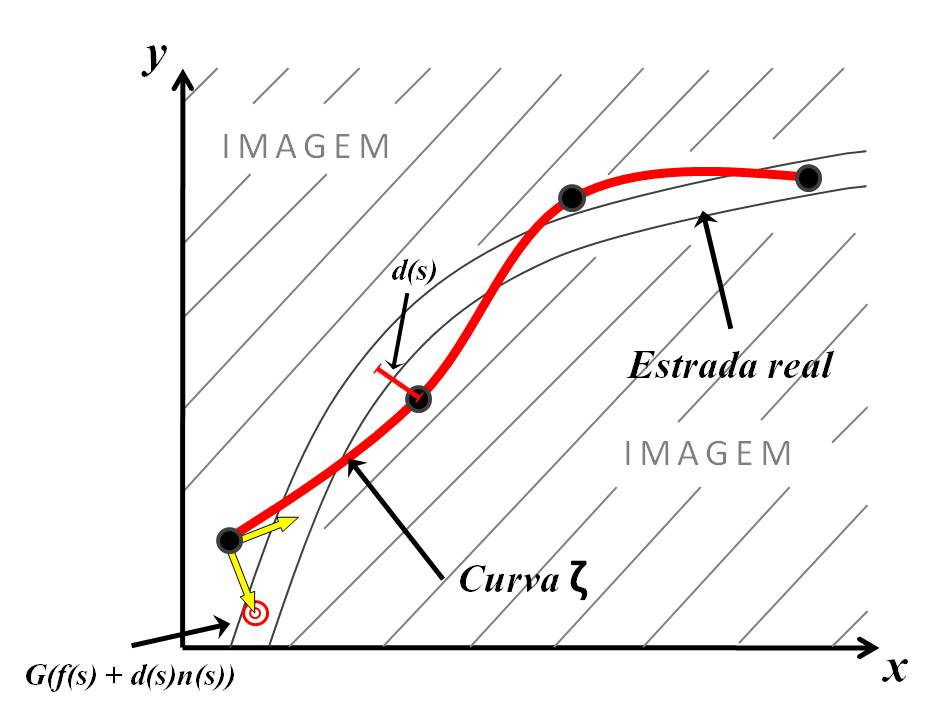
\includegraphics[width=0.63\textwidth]{figs/repreMatematica.jpg}}
    \caption{Ilustra��o da curva $\zeta$ sobre estrada em uma imagem digital, segundo propriedades matem�ticas definidas por \citeonline{gruen}.}
    \label{estradasReprMatematica}
\end{figure}
% Embora este tipo de imageamento possa trazer muitos benef�cios, h� ainda a necessidade de t�cnicas que minimizem o efeito do ru�do \emph{speckle}, comum a esse tipo de imagem e talvez o maior empecilho no reconhecimento dos padr�es. As pr�ximas se��es apresentam o processo de treinamento de uma RNA do tipo Kohonen, onde s�o apresentados os fundamentos da t�cnica e as heur�sticas utilizadas para o aprimoramento dos resultados. 

\section{Metodologia}
A sequ�ncia de apresenta��o desta se��o segue a l�gica de processamento do m�todo de extra��o de estradas apresentado. Cada um dos conceitos utilizados s�o dispostos em quatro se��es, detalhadas de acordo com o fluxograma na Figura \ref{fluxo2}. Primeiramente, emprega-se o m�todo de Semea��o; na segunda se��o, o m�todo de poda de pontos esp�rios e, na sequ�ncia, \emph{Snakes}. Por fim, na se��o M�tricas de Qualidade s�o apresentadas as medidas utilizadas para a avalia��o dos resultados.
\begin{figure}[htb]
    \centering
    \subfigure{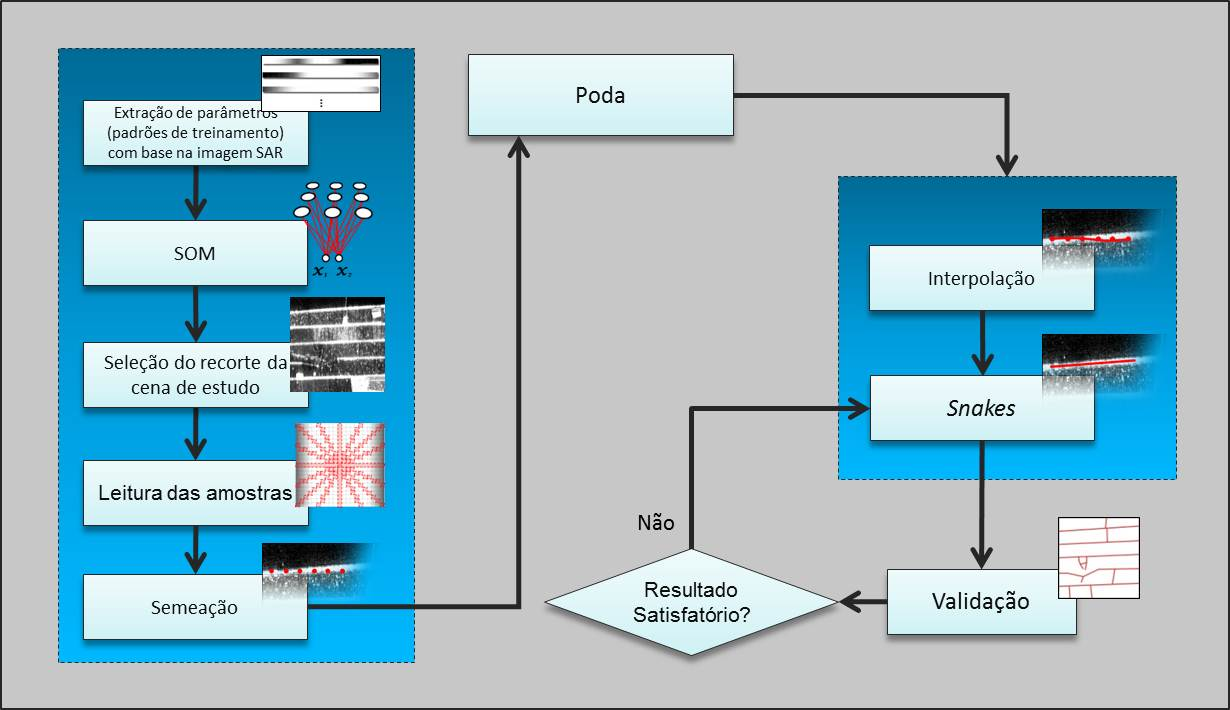
\includegraphics[width=0.96\textwidth]{figs/fluxograma.jpg}}
    \caption{Fluxograma do m�todo de extra��o de estradas.}
    \label{fluxo2}
\end{figure}

\subsection{Semea��o}\label{semeacao}
O m�todo de semea��o tem um papel importante no processo de extra��o de estradas. O procedimento consiste basicamente em identificar pontos que caracterizam a passagem de uma estrada na imagem. Como foi mencionado na se��o anterior, o m�todo de semea��o n�o � um m�todo de extra��o de estradas por si s�, embora sua utiliza��o tenha uma parcela importante no processo. Os pontos-sementes identificados nesta etapa interferem diretamente no m�todo \emph{Snakes}, pois uma vez que os pontos identificados estejam pr�ximos � fei��o de interesse, o m�todo de \emph{Snakes} tende a convergir rapidamente e eficientemente.

% Geralmente, a semea��o � categorizada como manual, semiautom�tica e 
% autom�tica. A primeira, e mais comum entre elas, necessita que um operador humano forne�a os pontos-sementes ao m�todo. Esta abordagem n�o possui
% qualquer liga��o com os recursos computacionais. A semea��o semiautom�tica possibilita ao operador humano alguns ajustes durante o processo 
% de identifica��o, al�m claro, do recurso computacional de detec��o. E por �ltimo, o processo de semea��o autom�tico � realizado de forma que 
% n�o haja quaisquer interfer�ncias humanas, sendo esta a mais complexa entre elas, justamente pela sua autonomia na identifica��o.

% � necess�rio que se defina as caracter�sticas das estradas a serem 
% identificadas no processo, considerando suas dimens�es, comprimento, propriedades espectrais, entre outros par�metros da RNA (ver Se��o 
% \ref{semeacaoSemi}). Tais propriedades a serem definidas previamente, faz com que o conceito se enquadre em um processo semiautom�tico. 
% Sendo assim, esse trabalho tem como objetivo apresentar um m�todo de extra��o de estradas em imagens de radar, cuja solu��o aborde o 
% m�todo de Semea��o semiautom�tico e Modelo de Contorno Ativo (\emph{Snakes}).
% A primeira parte da pr�xima se��o � destinada ao detalhamento destes par�metros. Em seguida, ser� apresentada a teoria envolvendo o m�todo 
% semiautom�tico, seu funcionamento e suas aplica��es.

Para que a semea��o tenha autonomia na identifica��o das estradas, � necess�rio atribuir a ela heur�sticas ou modelos que reconhe�am na imagem as caracter�sticas de sua forma. Para tanto, ser� utilizado um m�todo de reconhecimento de padr�es utilizando m�todos em Intelig�ncia Computacional, caracterizadas por simular, computacionalmente, os comportamentos e a aprendizagem humana. 

O processo de reconhecimento das formas presentes na imagem inicia-se apresentando-se � rede neural artificial todas os padr�es a serem reconhecidos, al�m daqueles que n�o caracterizam as fei��es de interesse. Neste trabalho, os padr�es de treinamento s�o definidos a partir da observa��o de perfis ideais de estrada em uma imagem SAR, em que s�o adquiridos os n�veis de intensidade de diferentes perfis. Ap�s a extra��o dos par�metros referentes ao conjunto de padr�es, � iniciada a etapa de treinamento da rede, processo detalhado na pr�xima se��o.

\subsubsection{\emph{Self-Organizing Maps - SOM}}\label{SecaoTreinamento}
Um dos primeiros modelos matem�ticos a simular a aprendizagem humana foi desenvolvido em 1943 por Warren McCulloch e Walter Pitts \cite{pitts}. Constitu�a-se de um conjunto de unidades processadoras de informa��o, denominados neur�nios ou n�s, interligados entre si, simulando uma rede neural. Mais tarde, em 1958, tal modelo foi estendido por Rosenblatt \cite{rosenblatt,rosenblatt2} e chamado de rede Perceptron, constitu�da por duas camadas de neur�nios, uma camada de entrada e outra de sa�da, de forma que cada neur�nio de uma camada era interligado com os da outra. Devido a esta estrutura, sua utiliza��o era limitada a resolver apenas problemas linearmente separ�veis. Diante de tais limita��es, fez necess�rio a cria��o de uma nova rede Perceptron com uma ou mais camadas intermedi�rias de neur�nios, o que possibilitaria a resolu��o de problemas mais complexos. A rede foi chamada de Perceptron de m�ltiplas camadas, ou simplesmente rede MLP (\emph{Mult-Layer Perceptron}). Este modelo possibilitou a resolu��o de problemas mais complexos.

Mais tarde, em 1982, surgiram os Mapas Auto-Organiz�veis (\emph{Self-Organizing Maps - SOM}), baseados no aprendizado n�o supervisionado, em que n�o � necess�rio apresentar � rede uma entrada e sa�da desejada para que ocorra o aprendizado. A ativa��o dos neur�nios � realizada em um processo de \textquotedblleft competi��o\textquotedblright$~$entre os mesmos, cujo lema � \textquotedblleft o vencedor leva tudo\textquotedblright, de modo que o neur�nio com menor est�mulo a uma determinada entrada � nomeado vencedor, tendo como recompensa o ajuste de seus pesos. 

As redes SOM s�o tamb�m chamadas de Mapas de Kohonen, em refer�ncia ao seu criador Teuvo Kohonen \cite{kohonen}. Sua arquitetura � constitu�da por apenas uma camada de entrada e uma de sa�da, sendo que esta �ltima representa o mapa de neur�nios (Figura \ref{arquiteturaSOM}). A ideia do Mapa de Kohonen remete ao funcionamento do c�rebro humano, onde cada regi�o � respons�vel por sentidos espec�ficos do corpo humano. Da mesma forma, os Mapas Auto-Organiz�veis s�o caracterizados pela forma��o de um mapa topogr�fico de padr�es de entrada, em que a localiza��o espacial do neur�nio na grade corresponde �s caracter�sticas intr�nsecas dos padr�es de entrada, justificando, assim, o nome do m�todo 
\cite{haykin}.
\begin{figure}[htb]
   \centering	       
    \subfigure{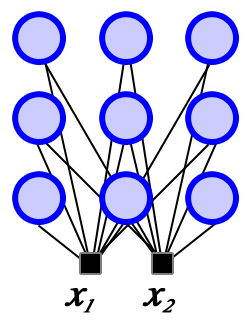
\includegraphics[width=0.17\textwidth]{figs/kohonen.jpg}}
    \caption{Exemplo de arquitetura de uma rede SOM, com mapa de sa�da bidimensional de dimens�o 3$\times$3 neur�nios e camada 
    de entrada com dois neur�nios ($x_1$ e $x_2$).}
    \label{arquiteturaSOM}
\end{figure}

Segundo \citeonline{haykin}, o processo de aprendizagem da rede SOM pode ser categorizada em tr�s etapas essenciais: competitivo, cooperativo e adaptativo. O primeiro diz respeito ao processo que define o neur�nio vencedor ou a determina��o do neur�nio que apresentou maior semelhan�a em rela��o ao vetor de entrada. No processo cooperativo, s�o definidos quais neur�nios, al�m do vencedor, ter�o seus pesos ajustados. Uma fun��o de vizinhan�a topol�gica � definida, de modo que satisfa�a a simetria entre o ponto m�ximo definido pelo neur�nio vencedor, sendo que a vari�vel de corre��o, deve decair conforme aumenta a dist�ncia do ponto central. As fun��es comumente utilizadas s�o a Chap�u Mexicano e a Gaussiana. Por fim, o processo adaptativo consiste no ajuste dos pesos em rela��o as entradas apresentadas. Estes tr�s processos comp�em o princ�pio b�sico do treinamento da rede SOM. Neste trabalho, adotou-se o processo cooperativo de aprendizagem, cuja fun��o Gaussiana � utilizada para a determina��o dos neur�nios vizinhos e posterior ajuste.

A efici�ncia dos resultados na etapa de semea��o reflete diretamente no resultado do m�todo \emph{Snakes}. Sendo assim, o processo de treinamento da RNA � considerado o mais importante nesta etapa, pois a partir dos valores obtidos aqui s�o gerados os pontos-sementes ao final da etapa. Os pontos devem ser marcados, pelo menos, pr�ximos �s fei��es que devem ser extra�das. No treinamento da RNA, s�o agregadas todas as formas que a rede dever� reconhecer, conforme as defini��es de estradas apresentadas na Se��o \ref{definicaoEstradas}. Em cada padr�o de treinamento s�o agregadas as caracter�sticas espec�ficas das estradas a serem reconhecidas, tais como largura, comprimento e n�veis de intensidade. 

Na defini��o dos padr�es de treinamento todas as informa��es dos objetos a serem identificados devem ser levados em considera��o, tais como as caracter�sticas de largura, orienta��o da estrada, n�veis de intensidade e comprimentos. Essas defini��es s�o importantes justamente pelas estradas aparecerem em diferentes formas na imagem. Levando em conta que o reconhecimento � aplicado sobre uma imagem de radar, as caracter�sticas que diferem uma estrada de um caminho devem ser levadas em conta, uma vez que tanto estradas como caminhos podem apresentar tonalidades claras ou escuras. Sendo assim, neste trabalho, adotou-se o total de oito padr�es de treinamento; sendo quatro deles tipos espec�ficos de estradas, em que s�o consideradas duas larguras a serem reconhecidas: tr�s \emph{pixels} e quinze \emph{pixels}, al�m de outros padr�es, id�nticos aos anteriores, por�m em n�veis de intensidade opostos, como forma de representa��o das estradas com tonalidades escuras. Os quatro �ltimos padr�es representam o que n�o � estrada na imagem, ou seja, padr�es nulos, utilizados para a classifica��o das amostras inv�lidas no reconhecimento (processo detalhado na Se��o \ref{classif}).

% Como os padr�es de treinamento foram definidos como perfis de estradas, a caracter�stica de orienta��o n�o foi considerada no treinamento. 
% Ao realizar o treinamento por perfil de estrada (21 valores) ao inv�s de um padr�o cheio (21x21 valores),
% reduziu-se o n�mero de n�s de entrada necess�rios para o treinamento da RNA, pois sendo o perfil de estrada constitu�do de 21 \emph{pixels} 
% (vetor de valores), � necess�rio uma rede com 21 n�s de entrada. Caso fosse utilizado um padr�o cheio como padr�o de treinamento, seriam 
% necess�rios n�o 21 n�s de entrada, mas sim 441 n�s (matriz 21x21). Contudo, � necess�rio que seja levado em conta a orienta��o da estrada no 
% reconhecimento. Caso ela n�o seja definida durante o treinamento, ela dever� ent�o ser definida na fase de reconhecimento. A Se��o 
% \ref{leituraAmostras} apresenta como este processo � tratado.

Como mencionado anteriormente, as RNAs do tipo Kohonen geralmente possuem somente uma camada de entrada e uma camada de sa�da, esta �ltima podendo ser unidimensional, bidimensional ou at� mesmo tridimensional. Neste trabalho, a camada de sa�da foi definida como um mapa bidimensional, onde cada elemento do mapa � conectado com os elementos de entrada $X_p$, em que $p$ � o �ndice do padr�o de treinamento. Cada uma dessas conex�es s�o representadas por um valor de pesagem, de forma que, cada elemento do padr�o de treinamento $X_p$ possua sua matriz de pesos $W$ correspondente. Desta forma, $W$ � uma matriz tridimensional $W_e$, tal que a dimens�o de $W_e$ � determinada pelo usu�rio. Na Figura \ref{esquemaRedeSOM} s�o ilustrados a arquitetura da rede SOM e suas respectivas vari�veis.
\begin{figure}[htb]
    \centering	   
    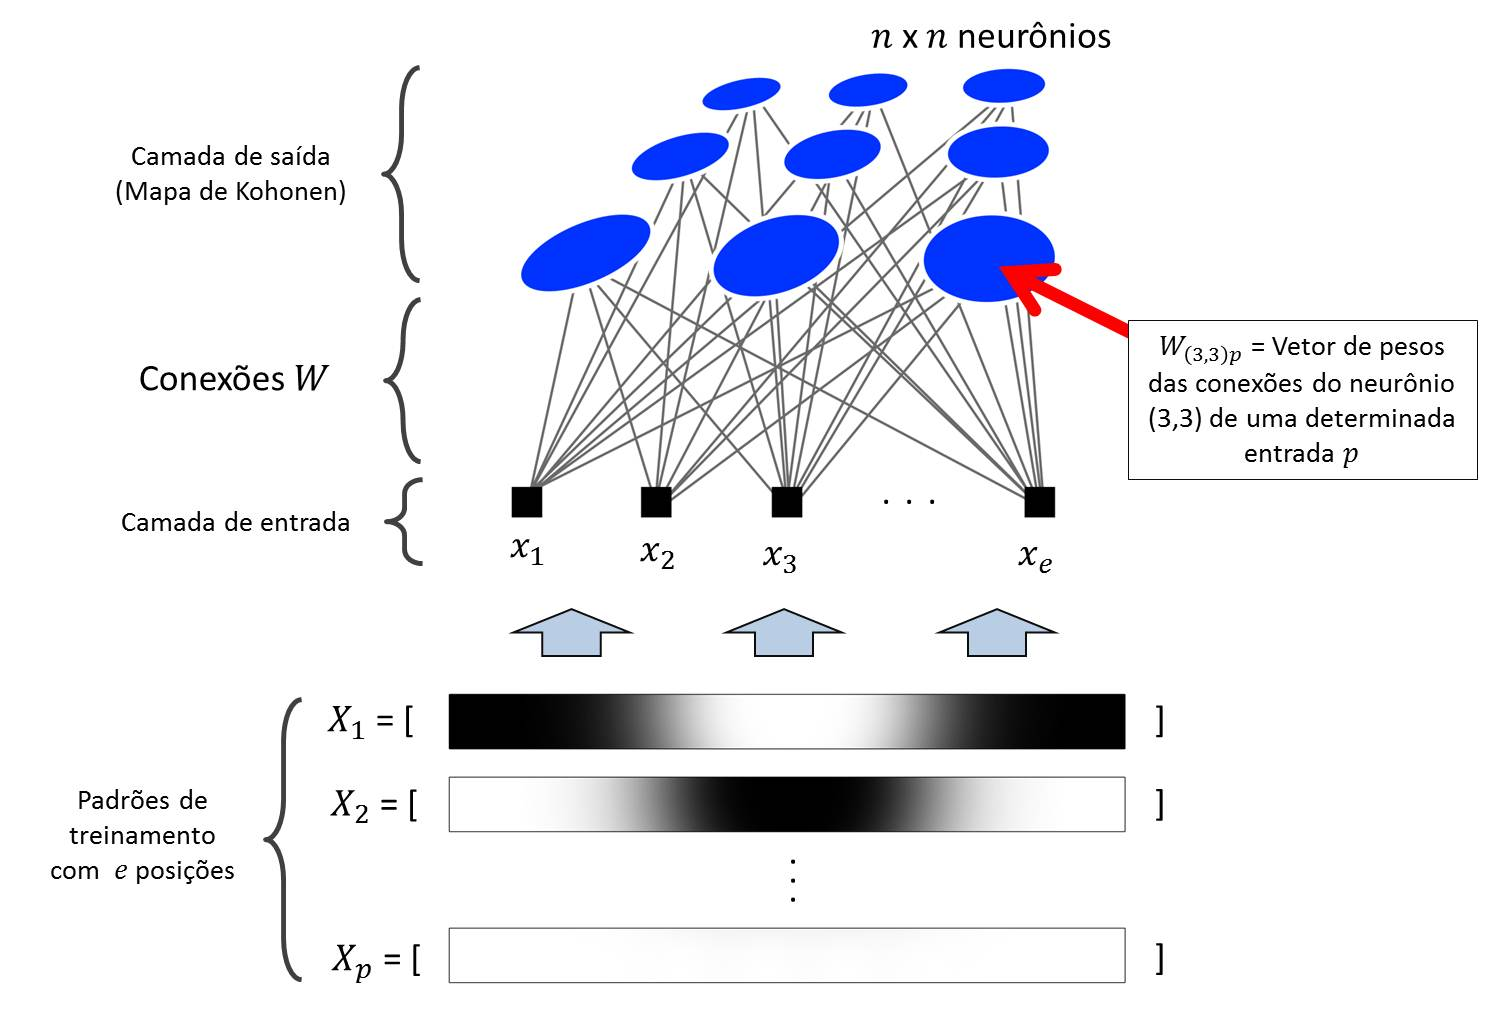
\includegraphics[width=0.8\textwidth]{figs/esquemaRedeSOM.jpg}
    \caption{Arquitetura da rede SOM empregada no trabalho, em que $e$ � igual a 21, $n$ igual a 6 e $p$ igual a 8.}
    \label{esquemaRedeSOM}
\end{figure}

Ap�s carregar os padr�es de treinamento, a matriz de pesos $W$ � ent�o iniciada. Geralmente, os valores de conex�es $W$ s�o iniciados aleatoriamente. � definido um valor m�ximo de itera��es, em que, a cada ciclo, os valores de $W$ s�o ajustados para que o mapa n�o seja formatado com uma tend�ncia inicial de se organizar. Esse processo de ajuste � denominado treinamento, em que, a cada ciclo de itera��o, � obtida a localiza��o do neur�nio de sa�da com menor dist�ncia euclidiana em rela��o � entrada apresentada. O c�lculo dessa dist�ncia � dado pela equa��o: 
\begin{align}
\label{eq1}
 i(X) = arg_{(j,k)}~min||W_{(j,k)} - X_p||~,~~~~
 \begin{cases}
    ~~~j = 1,2,...,n\\
    ~~~k = 1,2,...,n\\
 \end{cases}
\end{align}
em que $||.||$ denota a norma euclidiana entre os valores de entrada $X_p$ e $W_{(j,k)}$, correspondentes aos pesos de cada neur�nio $(j,k)$. $i(X)$ descreve a posi��o do neur�nio vencedor no mapa, dado por $arg_{(j,k)}$, e $n$ a raiz quadrada do n�mero de neur�nios na camada de sa�da \cite{haykin}. Ap�s obter a localiza��o do neur�nio vencedor, ou seja, o neur�nio que entre todos mais se assemelhou � entrada apresentada, s�o realizadas as corre��es da matriz de pesos $W_{(j,k)}$. Nesta etapa s�o corrigidos os valores do neur�nio vencedor e seus vizinhos. 

Por meio da Equa��o \ref{eq2} s�o realizadas as corre��es dos pesos, em que $\eta(t)$ � a taxa de aprendizagem da rede, a qual decai a cada itera��o ($t$). A vari�vel $\sigma$ denota a influ�ncia do neur�nio $(j,k)$ analisado, em rela��o ao vencedor, obedecendo um determinado raio de vizinhan�a. Na Figura \ref{figura3a} � ilustrado o mapa de neur�nios, na qual o c�rculo envolvendo os neur�nios vizinhos ao neur�nio vencedor, representa a vizinhan�a pela qual ocorrer�o os ajustes. Da mesma forma, na Figura \ref{figura3b} s�o demonstrados como seriam os valores de $\sigma$ para os neur�nios vizinhos, determinando a magnitude da corre��o dos neur�nios vizinhos; quanto maior o valor, maior a proximidade. Se o neur�nio n�o estiver pr�ximo o suficiente do neur�nio vencedor, sua influ�ncia ser� nula, e consequentemente, n�o ser� aplicado o ajuste. 
\begin{align}
\label{eq2}
 W(t+1)_{(j,k)} = W(t)_{(j,k)} + \eta(t) * \sigma_{(j,k)} * [X_p - W(t)_{(j,k)}]~.
\end{align} 

Os valores de $\sigma$ para um determinado neur�nio $(j,k)$ � dado pela propriedade gaussiana: 
\begin{align} 
 \label{eq3}
 \sigma_{(j,k)} = e^{-(\frac{dist}{2*raio^2})}~,
\end{align}
em que $dist$ representa a dist�ncia euclidiana entre o neur�nio vencedor e o neur�nio em quest�o, e $raio$, o raio de vizinhan�a. 

A taxa de aprendizagem decai a cada ciclo do treinamento. A fun��o que descreve o seu decaimento � dada por:
\begin{align}
 \eta(t) = \eta_0[e^{-(\frac{t}{T})}]~,
\end{align}
em que $\eta_0$ � a taxa de aprendizagem inicial, e $T$ � o n�mero m�ximo de itera��es. 
\begin{figure}[htb]
    \centering	   
    \subfigure[]{\label{figura3a}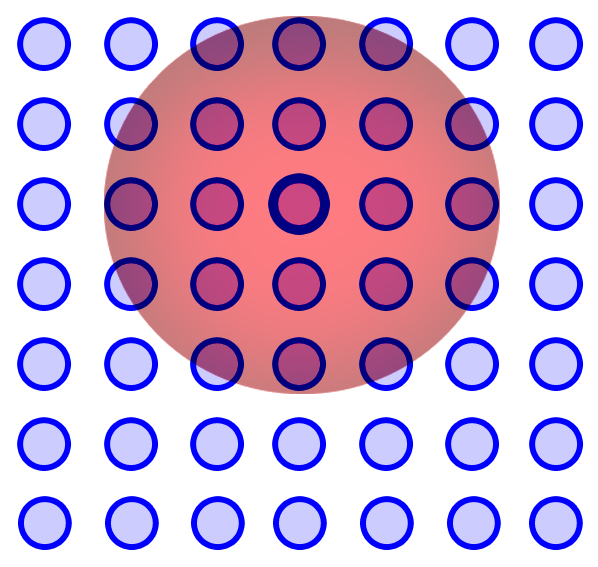
\includegraphics[width=0.29\textwidth]{figs/kohonen2.jpg}} \hspace{0.5cm}
    \subfigure[]{\label{figura3b}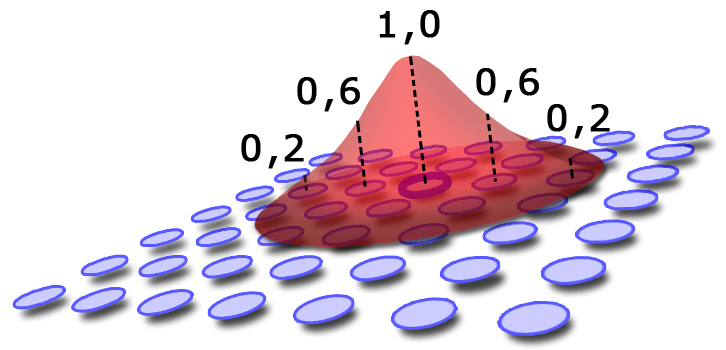
\includegraphics[width=0.46\textwidth]{figs/kohonen3.jpg}}
    \caption{Rede SOM: (a) Raio de vizinhan�a de um neur�nio vencedor. (b) Valores de $\sigma$ dos neur�nios vizinhos.}
    \FONTE{Adaptado de \citeonline{haykin}.}
    \label{figuraRedeKohonen}
\end{figure}

O processo de treinamento se encerra quando s�o conclu�das todas as itera��es $T$. Todo o processo de ajuste dos pesos de conex�es faz com que o mapa de Kohonen crie regi�es ou aglomerados (\emph{clusters}), sens�veis a padr�es espec�ficos, por meio das quais o treinamento foi realizado. Isto significa que o centro de cada uma dessas regi�es � sens�vel a um tipo espec�fico de informa��o, que diz respeito ao padr�o exato que foi apresentado. Sendo assim, seu entorno representa as formas que se assemelham a esse padr�o. 

Como exemplo, considere o c�rculo tracejado na Figura \ref{figura5ds} como sendo o aglomerado que corresponde a um padr�o de treinamento de perfil claro e entorno escuro, e largura aproximada de 6 \emph{pixels}. Ao apresentar � rede SOM amostras cujo valores se assemelhem com o respectivo padr�o de treinamento, o neur�nio vencedor tende a se localizar dentro desse c�rculo, quanto maior a semelhan�a, maior a proximidade do vencedor em rela��o ao centro do aglomerado.
\begin{figure}[htb]
   \centering   
   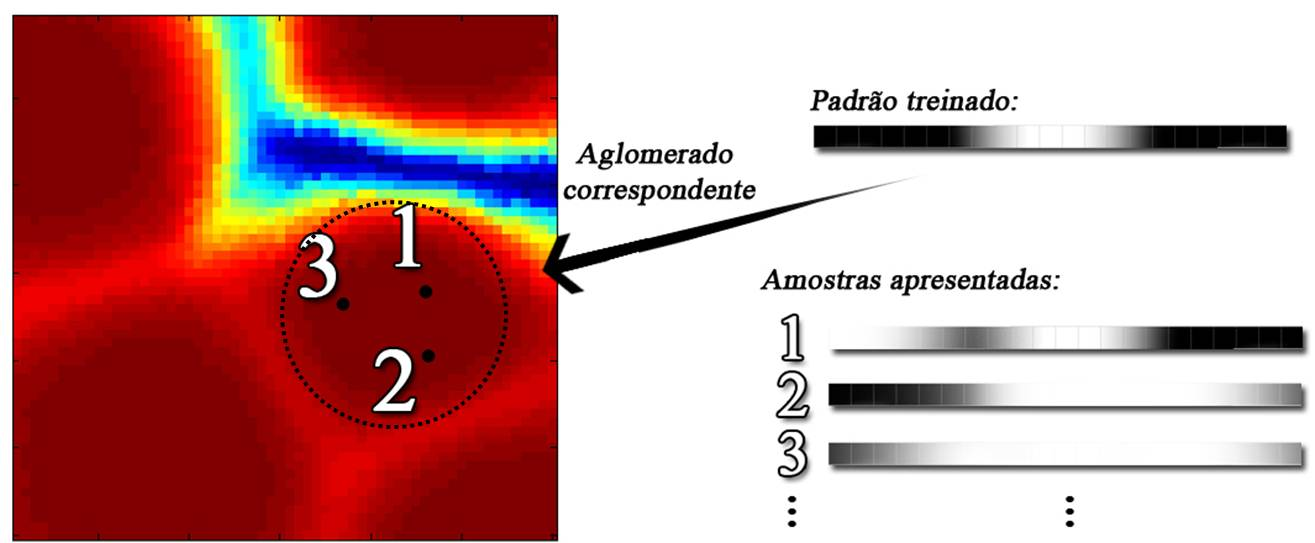
\includegraphics[width=0.77\textwidth]{figs/mapa_padroes_raio.jpg}
   \caption{Processo de classifica��o das estradas.}   
   \label{figura5ds}
\end{figure}

No dom�nio de Kohonen podem existir �reas pouco desenvolvidas no processo de treinamento, principalmente quando a dimens�o do mapa for relativamente grande. Neste caso, n�o h� garantias de que o vencedor ir� se localizar dentro de um determinado aglomerado Desta forma, � aconselh�vel que a dimens�o do mapa de Kohonen seja definida como a menor poss�vel, evitando a gera��o de regi�es de incertezas.

O mapa com as regi�es � dado pelos valores da matriz $W$, de forma que seus valores s�o unificados, caracterizando-se na Matriz Unificada ou Matriz U, representada por $W\_norm$. O c�lculo para a obten��o de $W\_norm$ � dado pela norma euclidiana de cada um dos pontos $W_{(j,k)}$ em rela��o a cada elemento de entrada $e$ de um padr�o de treinamento $p$. A Equa��o \ref{normEq} expressa o c�lculo de $W\_norm$, em que $E$ � o n�mero total de elementos de um determinado padr�o de treinamento. 
\begin{align}\label{normEq}
 W\_norm = \sqrt{\sum_{e=1}^E{(W_{e})^2}}~.
\end{align}

A Figura \ref{normFig} ilustra esse processo, no qual obt�m-se ao final o mapa da norma dos pesos (Matriz U). 
\begin{figure}[htb]
    \centering	       
    \subfigure{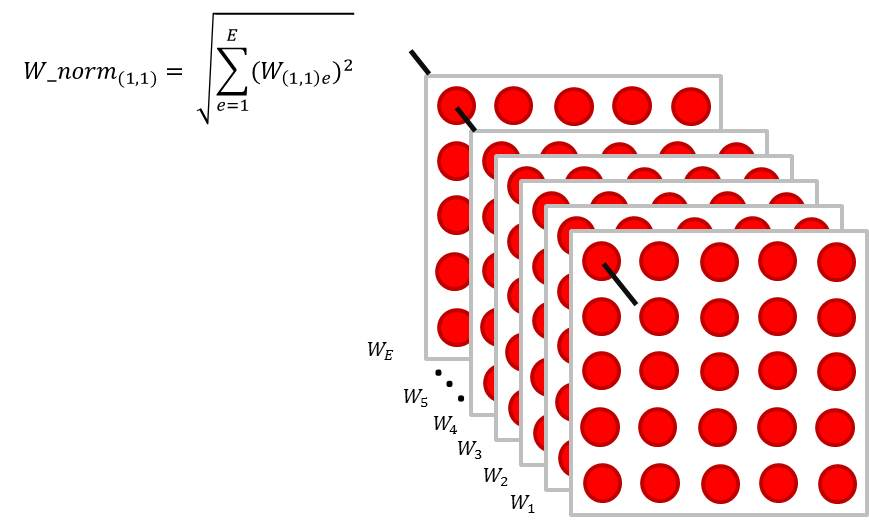
\includegraphics[width=0.66\textwidth]{figs/norma.jpg}}
    \caption{Pesos utilizados no c�lculo da norma para a montagem da Matriz U.}    
    \label{normFig}
\end{figure}

Ap�s o treinamento da rede SOM, o usu�rio seleciona a �rea de estudo a serem extra�das as estradas. Nessa �rea, � realizado o processo de leitura das amostras, processo detalhado na pr�xima se��o. Nesse etapa, o usu�rio pr�-determina o tamanho do salto da janela de leitura, sua dimens�o, e a quantidade de perfis a serem lidos em cada uma das amostras. 

\subsubsection{Leitura das Amostras}\label{leituraAmostras}
O processo de leitura das amostras consiste em varrer a imagem em saltos pr�-estabelecidos, de forma que, a cada salto uma janela de dimens�o fixa especifica o conjunto de \emph{pixels} que correspondem � respectiva amostra. A dimens�o da janela � fixada de acordo com os perfis de treinamento apresentados anteriormente � rede SOM. Neste caso, os perfis de treinamento possuem 21 elementos, consequentemente a dimens�o da janela � de 
21$\times$21 \emph{pixels}. A cada salto, s�o lidos os valores de diferentes orienta��es, como ilustrado na Figura \ref{orientacaoEstradas}. Em cada uma dessas orienta��es, s�o obtidos os perfis (vetor de valores), que, posteriormente, s�o utilizados na classifica��o ou identifica��o das estradas. 
\begin{figure}[htb]
   \centering	   
    \subfigure{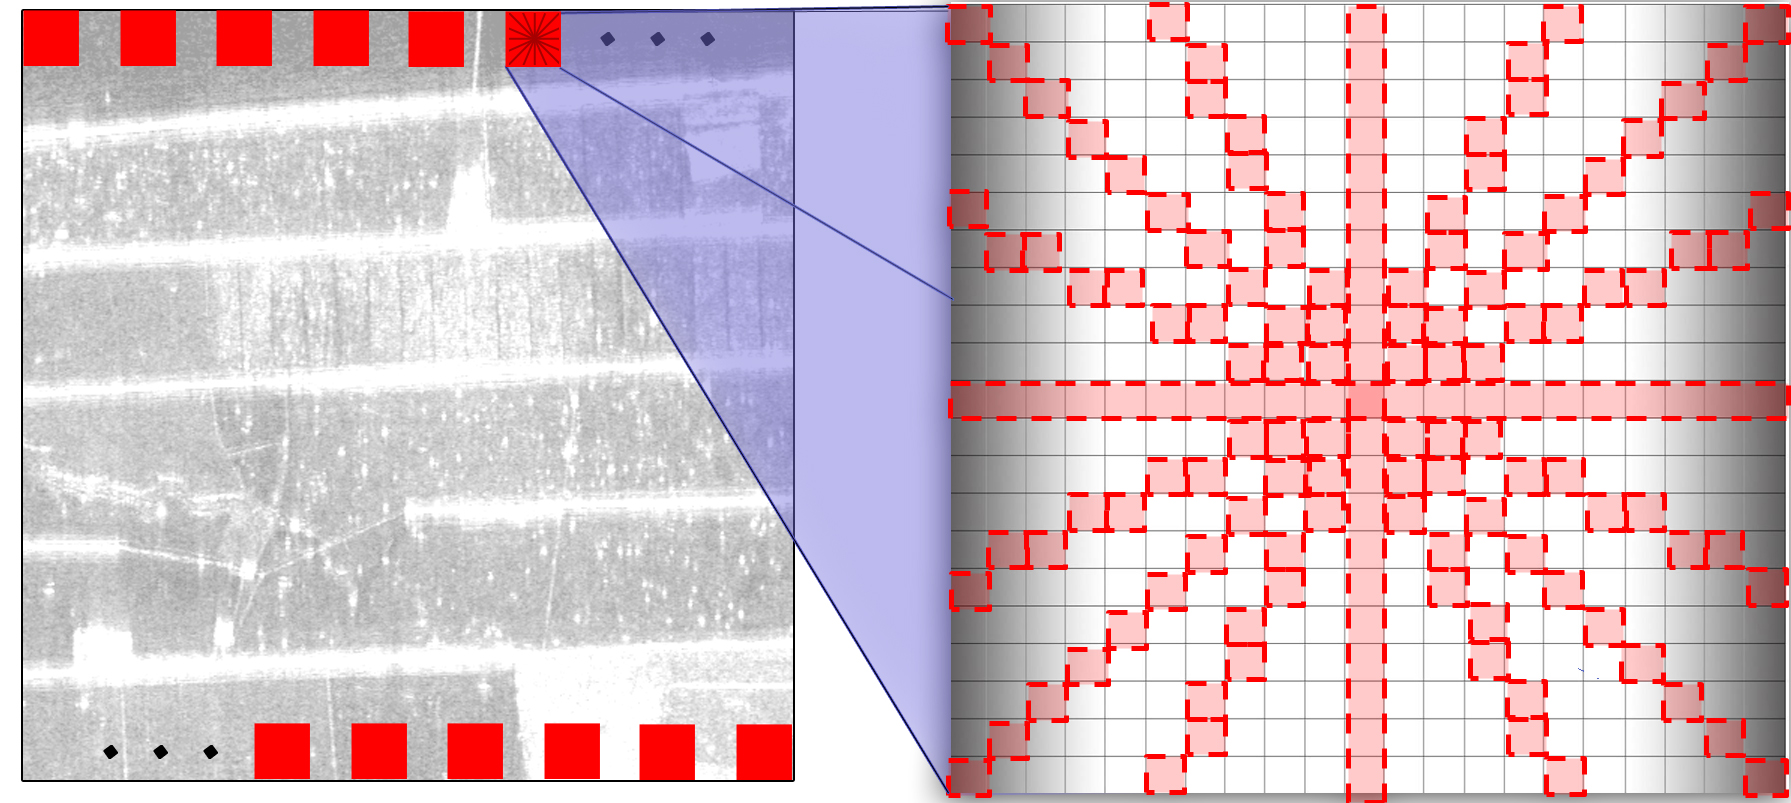
\includegraphics[width=0.66\textwidth]{figs/orientacoes3.jpg}} 
    \caption{Varredura da imagem para a leitura do conjunto $f$ de amostras, em que cada amostra, s�o obtidos $k$ perfis de estradas 
	    (Na ilustra��o, 8 perfis).}
    \label{orientacaoEstradas}
\end{figure}

Para a leitura das diferentes orienta��es na amostra, � necess�rio uma heur�stica para a determina��o dos \emph{pixels} em determinadas inclina��es de reta. O algoritmo do Ponto M�dio, conhecido tamb�m por algoritmo de Bresenham (\citeyear{bresenham}), determina justamente quais \emph{pixels} s�o renderizados, a fim de formar uma aproxima��o de uma linha reta entre dois pontos.

O algoritmo desenvolvido em 1965 por Jack E. Bresenham \cite{bresenham}, consiste em um m�todo simples para a obten��o de uma reta em um dispositivo matricial, tal como televisores e monitores. Dados dois pontos, ($x_0,y_0$) e ($x_1,y_1$), o primeiro representa o par de coordenadas do ponto inicial, e o segundo, o ponto final. O algoritmo se inicia a partir da determina��o da proje��o da reta, verificando especificamente as diferen�as entre as linhas final e inicial ($x_1 - x_0$), e colunas ($y_1 - y_0$), e com isso, determinar a inclina��o da reta. Para melhor compreens�o, na Figura \ref{bresenhamFig2}, � ilustrado o resultado da execu��o do m�todo, em que em cada coluna entre $x_0$ e $x_1$ h� exatamente um \emph{pixel} computado, enquanto que para cada linha entre $y_0$ e $y_1$ pode haver m�ltiplos \emph{pixels}. 
\begin{figure}[htb]
   \centering	   
    \subfigure{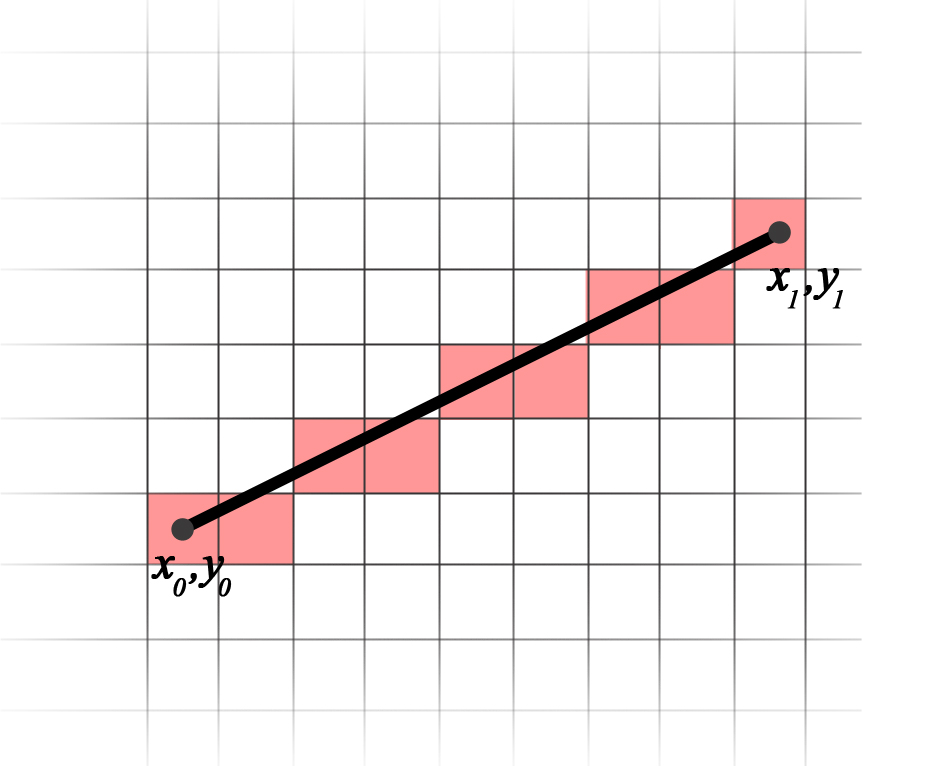
\includegraphics[width=0.39\textwidth]{figs/bresenham1.jpg}} 
    \caption{Exemplo da determina��o dos \emph{pixels} entre dois pontos em um dispositivo matricial (Algoritmo de Bresenham).}
    \label{bresenhamFig2}
\end{figure}
O algoritmo de Bresenham � utilizado neste trabalho para a leitura dos perfis em diferentes orienta��es (Figura \ref{orientacaoEstradas}), 
aumentando a chance de identificar a passagem de uma estrada, bem como a sua orienta��o na imagem.

O vetor de valores de cada uma das orienta��es possui, obrigatoriamente, a mesma quantidade de elementos que foram apresentados � rede. Para que a RNA aponte uma amostra como sendo uma estrada, pelo menos uma das orienta��es esteja pr�xima o suficiente de algum centro que corresponde a uma estrada. Isto �, pelo menos uma orienta��o deve estar no raio de algum dos aglomerados que representam o padr�o de estrada. Se pelo menos uma das orienta��es satisfizer essa condi��o, a amostra � identificada como sendo uma estrada. O c�lculo para a obten��o da orienta��o com menor valor � representado por:
\begin{align}\label{eq4}
 c(X) = arg_{orient}~min||W_{(j,k)} - X_{orient}||~,~~~~
 \begin{cases}
    ~~~orient &= 1,...,l\\
    ~~~j &= 1,2,...,n\\
    ~~~k &= 1,2,...,n\\
 \end{cases}
\end{align}
em que $X$ representa o conjunto dos valores para cada orienta��o, $orient$ � o �ndice da orienta��o, e $c(X)$ � o �ndice do vetor correspondente � orienta��o que mais se aproximou de um padr�o de estrada, e portanto, a orienta��o escolhida para a determina��o do ponto semente no processo de classifica��o. 

A se��o seguinte apresenta o m�todo de decis�o aplicado no reconhecimento das estradas, utilizando, essencialmente, a matriz de pesos obtida na etapa de treinamento, ou seja, as amostras lidas nessa etapa s�o apresentadas � RNA j� treinada, que, por sua vez, determina ou n�o a presen�a de estradas em seu conte�do.

\subsubsection{Classifica��o e Identifica��o}\label{classif}
Considerando que o treinamento da RNA tenha sido realizado adequadamente e as amostras da imagem lidas, o processo de reconhecimento ou identifica��o das estradas pode ent�o ser realizado. Cada amostra � apresentada � RNA treinada, para que esta fa�a o reconhecimento daquelas estradas que apresentarem padr�es semelhantes aos utilizados no treinamento. Como exposto na se��o anterior, ao apresentar uma determinada amostra para reconhecimento, seus valores s�o associados a uma posi��o no mapa de neur�nios, o que caracteriza o neur�nio vencedor para esse vetor de dados.

No treinamento da rede SOM neste trabalho, foram utilizados oito padr�es de treinamento. Os dois primeiros padr�es correspondem ao perfil de estrada larga (15 \emph{pixels}), sendo que o primeiro representa a estrada clara e entorno escuro, e o segundo, o inverso. Os dois padr�es seguintes correspondem a um perfil mais estreito de estrada (3 \emph{pixels}) e, assim como no caso dos dois primeiros padr�es, tamb�m s�o definidos com intensidades inversas. Por fim, os �ltimos quatro padr�es representam alvos que n�o correspondem a estradas.

A determina��o de uma amostra possuir ou n�o a passagem de uma estrada � dada pela apresenta��o de $c(X)$ (Equa��o \ref{eq4}) � rede SOM, em que � adquirido um neur�nio vencedor para a respectiva entrada. Caso esta esteja presente em um dos quatro aglomerados que dizem respeito ao padr�o estrada, a amostra � considerada como ponto-semente, caso contr�rio, ignorada. Os �ndices das amostras que forem selecionadas pelo m�todo de semea��o s�o armazenados. Tais �ndices s�o utilizados posteriormente em um processo de fragmenta��o, em que s�o selecionados os pontos-sementes pertencentes a um mesmo segmento de reta. Ao final do processo, � obtido uma matriz, tal que cada linha dessa corresponde aos �ndices das amostras pertencentes a um mesmo segmento de reta. A Figura \ref{indicesAmostras} ilustra as amostras identificadas como estrada no processo de classifica��o. 
\begin{figure}[htb]
   \centering	   
    \subfigure{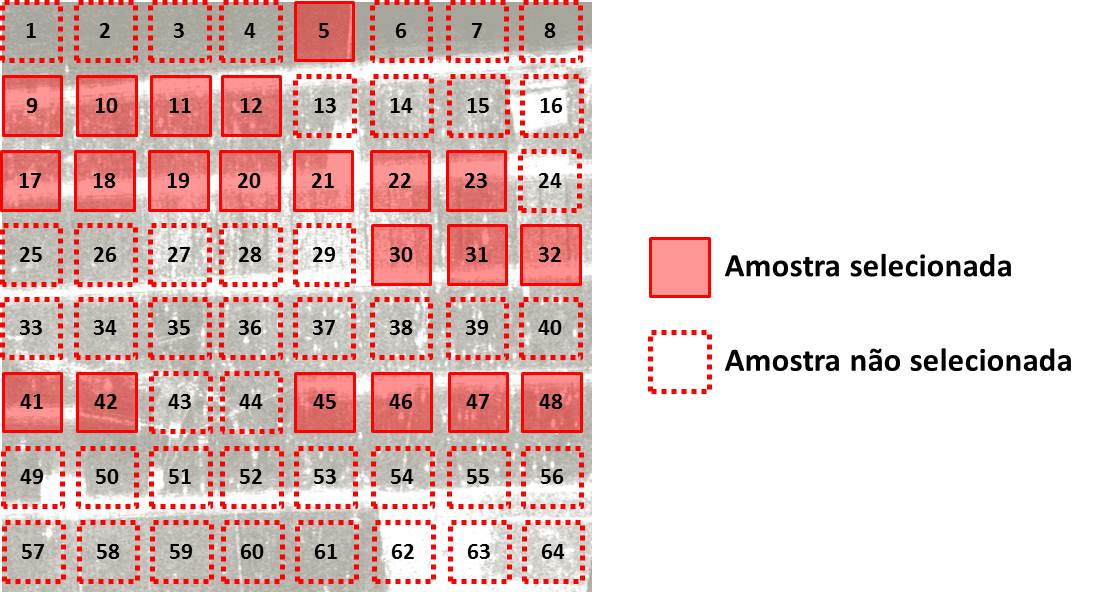
\includegraphics[width=0.69\textwidth]{figs/pontos-sementes.jpg}}     
    \caption{Exemplo do conjunto de amostras selecionadas pelo m�todo de semea��o.}    
    \label{indicesAmostras}
\end{figure} 
O vetor n�o fragmentado armazena sequencialmente os �ndices de cada amostra. Ao fragmentar este vetor, os �ndices ficam dispostos em uma matriz, de forma que cada linha caracteriza um conjunto de pontos-sementes pertencentes a um mesmo segmento de reta. Desta forma, o vetor fragmentado correspondente a Figura \ref{indicesAmostras} � dado por:
\begin{center} 
$
pontos =
\begin{bmatrix}
   9 & 10 & 11 & 12 & 0 & 0 & 0 \\
   17 & 18 & 19 & 20 & 21 & 22 & 23\\
   45 & 46 & 47 & 48 & 0 & 0 & 0
\end{bmatrix}
$
\end{center}

Na Se��o \ref{pruning} s�o apresentados os detalhes do processo de fragmenta��o e poda dos pontos-sementes.
% Desta forma, conclui-se que quatro dos oito padr�es apresentados � RNA caracterizam o que � estrada de fato. A utiliza��o dos padr�es 
% que n�o caracterizam estradas s�o �teis, pois com eles s�o criados as �reas de \textquotedblleft escape\textquotedblright$~$no pr�prio mapa de 
% neur�nios. Assim, ao analisar uma amostra que possua caracter�sticas muito distantes dos padr�es que representam estradas, o neur�nio 
% vencedor tender� a se localizar nessas �reas. Isso significa que a determina��o de uma amostra possuir ou n�o a passagem de uma estrada 
% fica mais flex�vel, uma vez que � obtida por meio da an�lise de sua localiza��o no dom�nio de Kohonen.

\subsection{Processo de poda dos pontos-sementes}\label{pruning}
Muitos dos pontos-sementes s�o marcados incorretamente, grande parte, em fun��o do ru�do presente na imagem. Como estrat�gia para a elimina��o destes pontos-sementes incorretos, foi desenvolvido um algoritmo de poda com o objetivo de separar todos os pontos que formam segmentos retos e cont�nuos, obedecendo algumas regras. Portanto, um conjunto de pontos-sementes � considerado como pertencente a um segmento de reta se as seguintes inequa��es se
verificam:
\begin{itemize} 
 \item \small $(f+1)~-~(f)~\leq$ \textbf{LMD}.
 \item \small \textbf{QPC} $\geq$ \textbf{LMC}.
\end{itemize}
Em que $f$ representa o �ndice das amostras identificadas, representando o ponto-semente propriamente dito. E os limiares LMC, LMD e QPC representam respectivamente:
\begin{itemize} 
 \item \small \textbf{Limite M�nimo de Continuidade}: Limiar que define a quantidade m�nima de pontos-sementes subsequentes para que sejam considerados como pertencentes a um mesmo segmento de reta.
 \item \small \textbf{Limite M�ximo de Descontinuidade}: Limiar que define a quantidade m�xima de descontinuidade entre os pontos-sementes para que sejam considerados como pertencentes a um mesmo segmento de reta.
 \item \small \textbf{Quantidade de Pontos Cont�nuos}: �ndice com o qual se verifica a continuidade dos pontos-sementes, caso este valor seja menor que LMC, a sequ�ncia � ignorada.
\end{itemize}
A Figura \ref{vetorFrag} ilustra um conjunto de pontos-sementes sobre uma estrada. Os pontos tracejados correspondem aos pontos-sementes n�o identificados na classifica��o, gerando as descontinuidades. Considerando o fator LMC igual a 4 e LMD igual a 2, somente os pontos: 6, 7, 8, 10 e 11 pertencem a um mesmo e �nico segmento de reta, pois entre os pontos 8 e 10 h� somente um ponto de descontinuidade, o que satisfaz a primeira condi��o, e o total de pontos-sementes � igual a 5 (QPC), o que satisfaz a segunda condi��o. Portanto, o conjunto de pontos-sementes � considerado como sendo um segmento de reta presente na imagem. Os pontos-sementes 1 e 2 satisfazem a primeira inequa��o, mas n�o a segunda, excluindo-se da classifica��o.
\begin{figure}[htb]
   \centering	   
    \subfigure{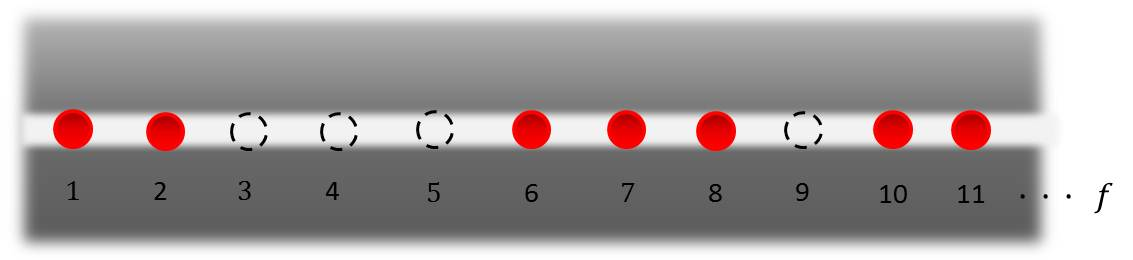
\includegraphics[width=0.75\textwidth]{figs/pruningProcess.jpg}} 
    \caption{Descontinuidades da classifica��o dos pontos-sementes.}
    \label{vetorFrag}
\end{figure} 

Ap�s este processo, tanto os pontos isolados apontados como uma estrada pelo m�todo quanto os segmentos de reta pequenos, s�o exclu�dos da identifica��o.

Nesta etapa do processo, os pontos-sementes est�o separados em grupos de segmentos de reta, dispostos em uma matriz. Nesta matriz, cada linha caracteriza um segmento de reta, e cada coluna dessas linhas, o �ndice da amostra (Figura \ref{vetorFrag}). Assim, para cada linha � aplicado o m�todo \emph{Snakes}, de forma que todos os elementos da linha s�o interpolados e aplicados ao m�todo. Ao t�rmino das linhas, � obtido ent�o a rede de estradas.

A semea��o realizada neste trabalho foi aplicada sobre a imagem de radar sem pr�-processamento, justamente para que se analisasse o comportamento do m�todo com a presen�a do ru�do (imagem original), apresentada no Cap�tulo \ref{capResultados}.

Nesta se��o \ref{semeacao}, foi apresentado como o processo de semea��o � realizado, sua fundamenta��o e import�ncia para o m�todo de extra��o de estradas. Na pr�xima se��o, ser�o apresentados detalhes do processo de obten��o do eixo de simetria das estradas pelo m�todo \emph{Snakes}.

\subsection{Modelo de Contorno Ativo (\emph{Snakes})}\label{snakes}
Embora a t�cnica tenha sido empregada no final da d�cada de 1980 por \citeonline{kass}, o termo Modelos Deform�veis surgiu em 1998 em um trabalho apresentado por \citeonline{terzopoulos}. A t�cnica consiste em obter formas (ou contornos) dos objetos presentes em uma imagem digital, permitindo 
que um contorno inicial se deforme e evolua para as bordas do objeto. Evolu��o esta que p�ra sob determinadas condi��es de convers�o, pr�-estabelecidas no modelo, e assim, sejam identificados os objetos presentes na imagem. 

Os modelos deform�veis s�o, em geral, considerados robustos pela sua capacidade em adaptar-se e identificar os objetos em cena com efici�ncia representando, portanto, uma contribui��o consider�vel para a Vis�o Computacional. Ap�s o surgimento da t�cnica, foram realizados diversos trabalhos que exploraram a maneira como os objetos eram reconhecidos \cite{cohen, osher, cootes, staib}. Basicamente, as solu��es apresentadas estendiam a maneira como a curva evolu�a em dire��o ao objeto, e essa evolu��o pode ser traduzida como a minimiza��o do funcional de energia da curva. Muitas solu��es se diferenciaram do m�todo variacional de Euler-Lagrange, apresentado por \citeonline{kass} para a minimiza��o da energia, e apresentaram t�cnicas igualmente boas, como, por exemplo, a utiliza��o da Programa��o Din�mica, apresentada por \citeonline{amini}, para a extra��o de estradas utilizando \emph{Snakes}, ou o m�todo de Fluxo do Vetor Gradiente (\emph{Gradient Vector Flow - GVF}) \cite{xu}, que, embora utilize o mesmo termo 
variacional, apresenta uma melhora consider�vel nos resultados quando as curvas iniciais s�o apresentadas distantes das fei��es a serem extra�das, 
o que � uma desvantagem no modelo tradicional.

A fim de que a curva venha a convergir para o contorno do objeto de maneira eficaz, � necess�rio que sua localiza��o se encontre pr�xima � fei��o de interesse. Por este fato, na maioria das vezes, o m�todo compreende um pr�-processamento manual, no qual um operador humano fornece pontos que se localizam pr�ximos � fei��o a ser extra�da. Esses pontos s�o ent�o interpolados, obtendo-se uma curva inicial. Ap�s a obten��o da curva inicial, essa � submetida a um processo iterativo para o c�lculo de sua nova localiza��o. Ao longo dessas itera��es, a curva se comporta de maneira semelhante a uma cobra (\emph{snake}), o que explica a raz�o do nome \cite{kass}.

Ao longo dos tempos, foram criadas diferentes varia��es do m�todo \emph{Snakes}. \citeonline{silvestre} relacionam as principais delas, tais como o m�todo \emph{Level Set}, que consiste em um modelo n�o-param�trico, cujo processo de identificar o contorno dos objetos n�o necessita de parametriza��o da curva \cite{osher}. Outra extens�o frequentemente abordada em trabalhos de reconhecimento de formas � o m�todo \emph{Balloon Snake} \cite{cohen}, no qual a curva evolui a partir do centro do objeto de interesse, imitando o comportamento de um bal�o de ar, ao contr�rio do que acontece no m�todo convencional, onde a curva inicial � formada ao redor do objeto.

Na Figura \ref{fluxo2} � ilustrada a metodologia usada na extra��o de estradas em imagens digitais. A partir de um conjunto de pontos provenientes do processo de Semea��o, os pontos-sementes, e a fragmenta��o desses em segmentos de reta, aplica-se o m�todo \emph{Snakes} para que seja realizada a extra��o da estrada, de forma que os pontos de um determinado segmento de reta s�o interpolados, obtendo-se, ent�o, uma curva inicial $\zeta$, tal como exemplificado na Figura \ref{estradasReprMatematica}.

Na se��o seguinte, � apresentada a fundamenta��o matem�tica da Teoria de \emph{Snakes}. As defini��es e equa��es apresentadas a seguir, s�o baseadas na teoria tradicional do m�todo, apresentada por \citeonline{kass}. Todas as adapta��es realizadas para a extra��o de estradas, s�o citadas juntamente com suas defini��es.

\subsubsection{Energia da \emph{Snake}}\label{energiaSnake}
Conforme exposto anteriormente, o problema do m�todo \emph{Snakes} se resume ao processo de minimiza��o de um funcional de energia. O modelo pode ser considerado como sendo uma \emph{spline} c�bica, controlada sobre a influ�ncia de suas energias interna e externa.

A curva $\zeta$ pode ser representada parametricamente por $v(s)=(x(s),y(s))$, em que $s$ � relacionado ao comprimento de arco, com valores crescentes ao longo da curva, $s\in[0,1]$, que se move no dom�nio espacial da imagem. O contorno ativo funciona pela minimiza��o da energia total da curva, $E_{snake}$, que � composta pela soma das energias interna, $E_{int}$, da imagem, $E_{image}$ e a energia $E_{con}$, imposta pelo usu�rio (Equa��o \ref{energiaTotal}). 
\begin{align}\label{energiaTotal}
 E_{snake} &= \int_0^1{E_{snake}(v(s))ds} \notag \\
 &= \int_0^1{[E_{int}(v(s)) + E_{ext}(v(s))]ds} \notag \\
 &= \int_0^1{[E_{int}(v(s)) + E_{image}(v(s)) + E_{con}(v(s))]ds}~.
\end{align}
Cada energia possui uma responsabilidade espec�fica no m�todo e, sendo assim, as se��es que se seguem destinam-se � apresenta��o das fun��es e defini��es de cada uma delas, exemplificando sua import�ncia em cada etapa da itera��o.

\subsubsection{Energia Interna}\label{energiaInternaCap}
A for�a interna � respons�vel por manter a rela��o de suavidade da curva, enquanto que a energia externa a impulsiona na dire��o de linhas,
bordas e contornos subjetivos \cite{kass}. A energia interna pode ser descrita por:
\begin{align}\label{energiaInterna}
%  E_{int}=\frac{1}{2}\int_0^1{\alpha(s)|v_s(s)|^2 + \beta(s)|v_{ss}(s)|^2 ds}~,
 E_{int} = \frac{1}{2} \int_0^1 \alpha(s) \left|\frac{\partial v(s)}{\partial s}\right|^2 + \beta(s)\left|\frac{\partial^2v(s)}{\partial s^2}\right|^2 ds~,
\end{align}
a qual � composta por dois termos: o termo de primeira ordem $\partial v(s)/\partial s$, controlado por $\alpha(s)$; e de segunda ordem 
$\partial^2 v(s)/\partial s^2$, controlado por $\beta(s)$. O termo de primeira ordem faz com que a curva se comporte como uma membrana, 
representando sua elasticidade. O segundo termo diz respeito � rigidez, agindo como uma placa fina, permitindo que, durante 
o processo de minimiza��o da energia, ela n�o se dobre \cite{kass}. As vari�veis $\alpha$ e $\beta$ podem ser consideradas como constantes, 
que funcionam como um fator de pondera��o, possibilitando o ajuste de acordo com as caracter�sticas da forma a ser identificada. Seus valores s�o essenciais 
para a efici�ncia do m�todo, ao passo que varia��es pequenas podem mudar significantemente o resultado \cite{bentabet}. \citeonline{agouris} 
mencionam que a escolha dos par�metros $\alpha$ e $\beta$ pode ser realizada empiricamente, definindo-os de acordo com as caracter�sticas 
da imagem ou fei��es a serem extra�das. \citeonline{bentabet} utilizaram valores de $\beta$ estimados automaticamente, em que inicialmente 
s�o verificadas as caracter�sticas predominantes das fei��es por meio de uma base de dados com a verdade terrestre das mesmas, e ent�o, 
obt�m-se o valor m�dio da curvatura dessas fei��es. A partir dessa informa��o, estima-se o valor de $\beta$. 

% A Figura \ref{snake1} ilustra o resultado final da \emph{snake} para diferentes valores de $\alpha$.
% \begin{figure}[htb]
%     \centering	   
%     \subfigure[]{\label{snake1a}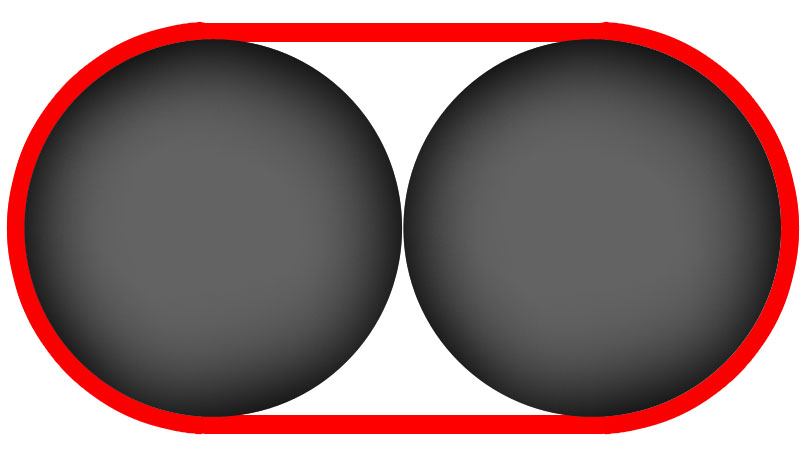
\includegraphics[width=0.28\textwidth]{figs/snake1a.jpg}} \hspace{0.3cm}    
%     \subfigure[]{\label{snake1b}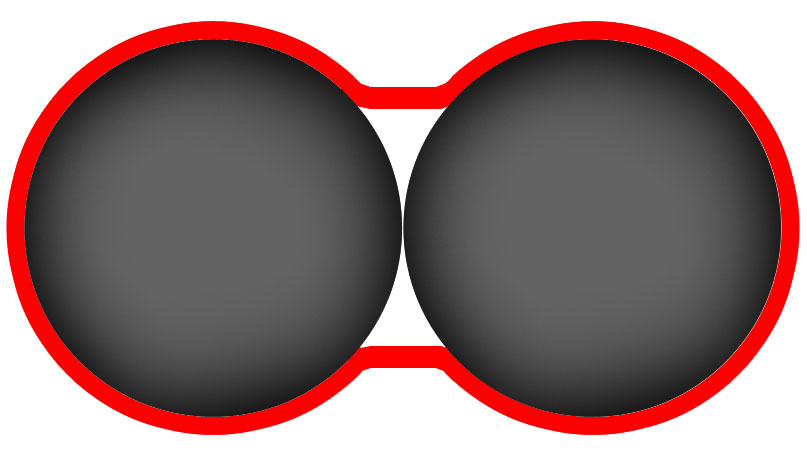
\includegraphics[width=0.28\textwidth]{figs/snake1b.jpg}} \hspace{0.3cm}
%     \subfigure[]{\label{snake1c}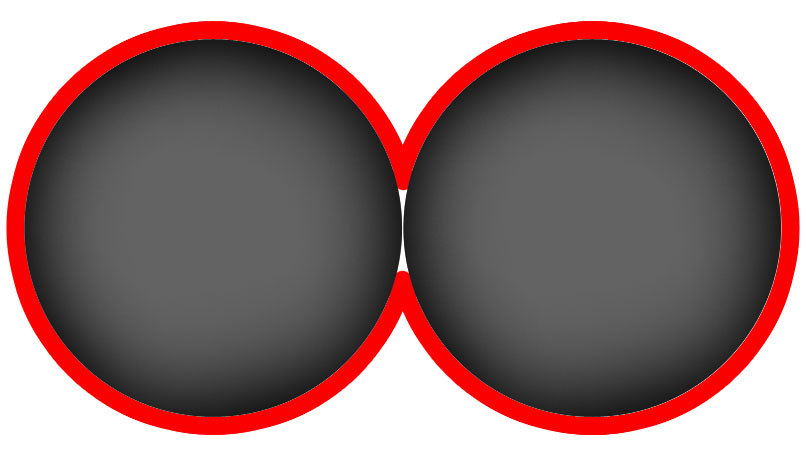
\includegraphics[width=0.28\textwidth]{figs/snake1c.jpg}} \\
%     \caption{Exemplo da evolu��o da \emph{snake} para diferentes valores de $\alpha$: (a) Valor alto. (b) Valor mediano. (c) Valor baixo.}
%     \FONTE{Chris Bregler and Malcolm Slaney \citeyear{bregler}}
%     \label{snake1}
% \end{figure}
% A constante $\beta$ especifica a rigidez do contorno. Desta forma, valores baixos de $\beta$ faz com que a curva desenvolva pontos de descontinuidade 
% na identifica��o.

As fun��es $\partial v(s)/\partial s$ e $\partial^2 v(s)/\partial s^2$, que comp�em cada um dos termos, s�o as derivadas de primeira e segunda 
ordem de $v(s)$, respectivamente. A primeira fornece o coeficiente angular tangente � curva no ponto $s$, e a segunda, o vetor normal a este 
ponto. A Equa��o \ref{energiaInterna} n�o admite qualquer solu��o anal�tica, fazendo com que seja requerido um processo iterativo para 
resolv�-la. O mais comum dos processos � o m�todo de Euler-Lagrange, em que a Equa��o \ref{energiaInterna} � reescrita na equa��o de Euler, 
correspondendo assim a uma equa��o de equil�brio ou de minimiza��o \cite{bentabet}. O processo de minimiza��o � apresentado na Se��o 
\ref{minizacaoEnergia}.

\subsubsection{Energia externa}\label{energiaImagemCap}
A soma das energias $E_{image}$ e $E_{con}$ � denominada energia externa $E_{ext}$. A energia da imagem, $E_{image}$, � composta pela soma do produto de tr�s outras energias.
\begin{align}\label{energiaImagem}
  E_{image} = w_{line}E_{line} + w_{edge}E_{edge} + w_{term}E_{term}~.
\end{align}
Os valores de $w_{line}$, $w_{edge}$ e $w_{term}$ s�o constantes que funcionam como ajustes para suas respectivas energias. $E_{line}$ especifica as caracter�sticas do contorno quanto aos n�veis de intensidade da forma, ou seja, dependendo do valor de $w_{line}$, a curva ser� atra�da por linhas claras ou escuras. Tal energia refere-se simplesmente aos n�veis de intensidade da imagem. Na abordagem original apresentada por \citeonline{kass}, s�o apresentadas duas representa��es do funcional de linha. Na Equa��o \ref{energiaLine1}, a primeira apresentada pelos autores, a curva � atra�da por contornos com gradientes altos de imagem, em que a curva tende a convergir na borda do objeto.
\begin{align}\label{energiaLine1}
 E_{line} = I(x,y)~.
\end{align}
A segunda representa��o � dada por:
\begin{align}\label{energiaLine2}
 E_{line} = -(G_{\sigma}*\nabla^2I)^2~,
\end{align}
em que $G_{\sigma}$ representa uma Gaussiana de desvio padr�o $\sigma$, e $\nabla^2I$ o gradiente de segunda ordem da imagem. Ambas permitem adquirir o contorno do objeto sendo que, a segunda representa��o se difere pelo comportamento da curva em ser atra�da � regi�es de passagem-por-zero (\emph{zero-crossing}), isto �, regi�es com mudan�as bruscas de intensidade.

O funcional de borda, $E_{edge}$, pode ser interpretado tamb�m como um operador para a identifica��o de bordas na imagem, e � dado por:
\begin{align}\label{energiaEdge}
 E_{edge} = -|\nabla I|^2~,
\end{align}
em que $\nabla I$ � o gradiente da imagem $I$ e, $E_{term}$ � definido por \citeonline{kass} como o funcional de limite que, tem como responsabilidade de encontrar termina��es e cantos dos segmentos de reta. Para tanto, utiliza-se o n�vel de curvatura das linhas da imagem ap�s suaviza��o, dada por um filtro gaussiano: 
\begin{align}
C(x,y)=G_{\sigma}(x,y)*I(x,y)~, 
\end{align}
O n�vel de curvatura pode ser obtido pelo c�lculo da varia��o do �ngulo gradiente em rela��o ao vetor perpendicular ao gradiente:
\begin{align}
 E_{term} &= \frac{\partial\theta}{\partial n_{\bot}} \\ 
 &= \frac{\partial^2C / \partial n_{\bot}^2}{\partial C / \partial n} \\
\label{energiaTerm3}
 &= \frac{C_{yy}C_x^2-2C_{xy}C_xC_y+C_{xx}C_y^2}{(C_x^2+C_y^2)^{\frac{3}{2}}}~,
\end{align}
em que $\theta=tan^{-1}(C_y/C_x)$ � o �ngulo do gradiente, $n = (cos\theta,sen\theta)$ e $n_{\bot}=(-sen\theta,cos\theta)$ s�o vetores unit�rios na dire��o do gradiente e perpendicular a este, respectivamente. A Equa��o \ref{energiaTerm3} representa a solu��o discreta do c�lculo dos n�veis de curvatura das linhas na imagem, que em termos pr�ticos, $C_x$, $C_y$ e $C_{xy}$ representam as diferen�as discretas avan�adas de primeira ordem da imagem suavizada $C(x,y)$ em rela��o aos respectivos eixos $x$ e $y$, que caracterizam-se em uma imagem com realces de borda do tipo degrau com orienta��o em $x$, do tipo degrau com orienta��o em $y$ e do tipo degrau com orienta��o nos dois eixos, respectivamente. Os termos $C_{xx}$ e $C_{yy}$ correspondem �s diferen�as discretas avan�adas de segunda ordem, obtendo uma imagem com realces de borda do tipo cartola (\emph{top-hat}) com orienta��o em $x$ e $y$, respectivamente \cite{hoffman}. A combina��o do funcional de termina��o $E_{term}$, com o funcional de borda $E_{edge}$, faz com que a curva evolua n�o s� para os contornos do objeto, como tamb�m para regi�es onde n�o h� contornos reais, mas sim fict�cios. Na Figura \ref{snake2}, � ilustrado a evolu��o da curva para as bordas do objeto, que, apesar de n�o existirem de fato, s�o reconhecidas pelo m�todo.
\begin{figure}[htb]
    \centering	     
    \subfigure[]{\label{snake2a}
\includegraphics[width=0.21\textwidth]{figs/snake1process.jpg}} \hspace{0.1cm}        
    \subfigure[]{\label{snake2b}
\includegraphics[width=0.21\textwidth]{figs/snake2process.jpg}} \hspace{0.1cm}  
    \subfigure[]{\label{snake2c}
\includegraphics[width=0.21\textwidth]{figs/snake3process.jpg}} \hspace{0.1cm}
    \subfigure[]{\label{snake2d}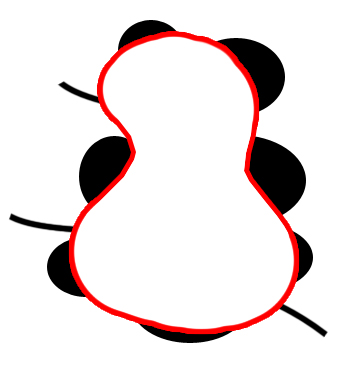
\includegraphics[width=0.21\textwidth]{figs/snake4process.jpg}} \\
    \caption{Exemplo da obten��o de contornos criados pela \emph{Snakes}: (a) Imagem original. (b) Curva inicial. 
	     (c) Evolu��o intermedi�ria da curva. (d) Curva final.}
    \FONTE{Adaptado de \citeonline{kass}.}
    \label{snake2}
\end{figure}

Por fim, o par�metro $E_{con}$, na Equa��o \ref{energiaTotal}, � definido como sendo uma energia de restri��o imposta pelo usu�rio. Muitas vezes, esse termo n�o � utilizado no processo de extra��o de estradas, como apresentado em \citeonline{bentabet, agouris} e \citeonline{youn}. Assim como a energia de restri��o $E_{con}$, outros trabalhos negligenciam o uso das energias $E_{edge}$ e $E_{term}$ justamente por n�o serem �teis, face �s caracter�sticas do objeto a ser extra�do. A aplica��o de \emph{Snakes} apresentada neste trabalho dispensa o uso dos termos $E_{con}$, $E_{term}$ e $E_{edge}$. O �ltimo termo � desprezado, uma vez que o objetivo � obter o centro das vias e n�o suas bordas. Portanto, a Equa��o \ref{energiaTotal} � reescrita:
\begin{align}
E_{snake} &= E_{int} + E_{image} \notag \\
&= E_{int} + w_{line}E_{line}
\end{align}

O processo de obten��o dos eixos de simetria das vias � definido como sendo um procedimento de minimiza��o da energia total da curva (Equa��o 
\ref{energiaTotal}). Existem diferentes maneiras de se minimizar tal energia. Na se��o seguinte, ser�o apresentadas as principais t�cnicas 
utilizadas para a resolu��o deste problema.

\subsubsection{Minimiza��o da Energia Total}\label{minizacaoEnergia}
Nas se��es anteriores, foram apresentadas as caracter�sticas gerais da curva, entre as quais a representa��o no 
dom�nio espacial, definida como uma curva parametrizada por um conjunto de pontos no plano ($x,y$) da imagem, denotada por $v(s)$. 
De forma que a obten��o do contorno de um determinado objeto � dado pela minimiza��o de $v(s)$, que corresponde � busca do m�nimo
local da soma de suas energias, representada pela Equa��o \ref{energiaSnake}, a qual n�o admite solu��o anal�tica, o que equivale 
dizer que, para o problema da minimiza��o da curva, a equa��o anterior deve ser reescrita de forma que num esquema iterativo 
possa-se encontrar solu��es para ela.

Segundo \citeonline{bentabet}, m�todos como Algoritmos Gananciosos (\emph{Greeding Algorithm}) e Otimiza��o por Arrefecimento Simulado 
(\emph{Simulated Anealing}) s�o tipos requeridos para a solu��o do problema de minimiza��o. Esses algoritmos s�o utilizados na busca de 
m�nimos globais que representam pontos de estabilidades ou de equil�brio em um determinado problema de otimiza��o, tal como a minimiza��o 
do funcional de energia, $E_{snake}$. A Programa��o Din�mica \cite{bellman} � outra alternativa para a obten��o do m�nimo de $E_{snake}$ 
\cite{amini, gruen, liThesis, dalpoz3}.

O m�todo mais comum de minimiza��o do funcional de energia, � reescrito como uma equa��o de \emph{Euler-Lagrange}, correspondendo � uma 
fun��o de equil�brio \cite{kass,bentabet,laptev,haupt}, tal que a minimiza��o do funcional de energia na Equa��o \ref{energiaInterna} d� 
origem a duas novas equa��es de Euler independentes.
\begin{align}
 \label{euler1}
 \alpha(s) \frac{\partial^2 x(s)}{\partial s^2} + \beta(s) \frac{\partial^4 x(s)}{\partial s^4} + \frac{\partial E_{ext}}{\partial x} &= 0~, \\ 
 \label{euler2}
 \alpha(s) \frac{\partial^2 y(s)}{\partial s^2} + \beta(s) \frac{\partial^4 y(s)}{\partial s^4} + \frac{\partial E_{ext}}{\partial y} &= 0~,
\end{align}

Para \citeonline{laptev}, os equil�brios entre a energia interna e a energia da imagem s�o importantes no processo de minimiza��o. Se uma delas tiver dom�nio sobre a outra, anular� a rela��o de suavidade da curva ou a for�ar� a ignorar a energia da imagem, sendo que ambos efeitos s�o indesejados. Desde que a energia interna possa ser controlada, o equil�brio pode ser alcan�ado com o ajuste preciso de $\alpha(s)$ e $\beta(s)$. Sendo assim, \citeonline{laptev} utilizaram a id�ia apresentada por \citeonline{fua}, os quais criaram uma maneira de automatizar a defini��o dos valores de $\alpha(s)$ e $\beta(s)$, em que se substituem as fun��es por uma constante $\lambda$.

Resolver as Equa��es \ref{euler1} e \ref{euler2} computacionalmente implica dizer que a evolu��o da curva pode ser realizada somente em per�odo discreto de tempo. Assim, � necess�ria a discretiza��o da representa��o da \emph{snake} a fim de aproximar sua posi��o e derivadas \cite{laptev}. Uma abordagem que oferece a discretiza��o precisa de derivadas � dada pelo m�todo de diferen�as finitas \cite{bentabet}. Na resolu��o apresentada por \citeonline{kass}, aproximando-as pelo m�todo de diferen�as finitas, considera-se:
\begin{align}
 v_i=(x_i,y_i)=(x_i(s,t),y_i(s,t))~,~~~~i = 1,...,n~;    
 \end{align}
em que $s$ denota o par�metro do comprimento de arco, $t$, a vari�vel temporal e $i$ o �ndice do ponto na curva. Neste caso, a expans�o da energia interna do \emph{i}-�simo v�rtice � dada por: 
\begin{align}
 E_{int}(i) = \frac{\alpha_i|v_i - v_{i-1}|^2}{2s^2} + \frac{\beta_i|v_{i-1}-2v_i + v_{i+1}|^2}{2s^4}~.
\end{align}
Considerando as derivadas parciais da energia externa em rela��o a $x$, $f_x(i) = \partial E_{ext} / \partial x_i$, e em rela��o a $y$, $f_y(i) = \partial E_{ext} / \partial y_i$, em cada v�rtice $v_i$, as equa��es de Euler Lagrange, de acordo com o c�lculo variacional \cite{courant}, podem ser assim apresentadas, j� considerando o m�todo de diferen�as finitas:
\begin{align}\label{discrEuler}
 \alpha_i(v_i - v_{i-1}) - &\alpha_{i+1}(v_{i+1} - v_i) \notag \\
			   &+ \beta_{i-1}[v_{i-2} - 2v_{i-1} + v_i] \notag \\
			   &- 2\beta_i[v_{i-1}-2v_i + v_{i+1}] \notag \\
			   &+ \beta_{i+1}[v_i - 2v_{i+1} + v_{i+2}] \notag \\
			   &+ (f_x(i),f_y(i)) = 0~.
\end{align}
A Equa��o \ref{discrEuler} pode ser reescrita na forma matricial:
\begin{align}
 Ax + f_x(x,y) &= 0~,\\
 Ay + f_y(x,y) &= 0~,
\end{align}
em que $A$ � uma matriz penta-diagonal sim�trica $n\times n$, dada pelos coeficientes da Equa��o \ref{discrEuler}. Devido as derivadas parciais da energia externa utilizada, s�o necess�rias mudan�as em $A$ a cada itera��o. Por simplicidade, admita-se que $f_x$ e $f_y$ s�o constantes durante um intervalo de tempo, o que origina o m�todo expl�cito de Euler em rela��o � energia externa. A energia interna, entretanto, � especificada pela matriz $A$, assim, � poss�vel validar a derivada temporal no tempo $t$, ao inv�s de $t-1$ e, consequentemente, obter um passo impl�cito de Euler para as energias internas, resultando em:
\begin{align} 
 \label{eq15}
 Ax^{(t)} + f_x(x^{(t-1)}, y^{(t-1)}) = -\gamma(x^{(t)} - x^{(t-1)})~,\\
 \label{eq16}
 Ay^{(t)} + f_y(x^{(t-1)}, y^{(t-1)}) = -\gamma(y^{(t)} - y^{(t-1)})~,
\end{align}
em que $\gamma$ � o tamanho do passo, $x^{(t)}$ e $y^{(t)}$ s�o vetores colunas $n\times1$, correspondendo �s localiza��es dos pontos $v$ no tempo $t$ e o termo $f(.)$ denota as derivadas parciais dos pontos no tempo $t-1$ que, por sua vez, corresponde tamb�m a um vetor coluna $n\times1$. Isolando-se as vari�veis $x$ e $y$ tem-se:
\begin{align} 
 x^{(t)} = (A + \gamma I)^{-1} (\gamma x^{(t-1)} - f_x(x^{(t-1)}, y^{(t-1)})~,\\
 y^{(t)} = (A + \gamma I)^{-1} (\gamma y^{(t-1)} - f_y(x^{(t-1)}, y^{(t-1)})~,
\end{align}
em que $I$ � uma matriz identidade $n\times n$, assim, a matriz $A + \gamma I$ � uma matriz penta-diagonal, podendo simplesmente ser invertida pelo m�todo de decomposi��o \emph{LU}.

\subsubsection{Representa��o Aberta da Curva \emph{Snake}}\label{curvaAberta}
Existem duas importantes configura��es da curva a serem consideradas: as de car�ter fechado e as de car�ter aberto. At� ent�o, foram apresentadas as defini��es para a curva fechada (la�o), assim como a defini��o em sua base original. Tratando-se da extra��o de fei��es lineares, fica evidente que a configura��o da curva necessita ser aberta. Seria impratic�vel utilizar a base tradicional do m�todo, que apresenta as defini��es para a curva fechada, como um extrator de estradas, e ainda, obter um bom resultado. Encontram-se na literatura muitos trabalhos abordando a extra��o de estradas com o uso da curva aberta, por�m, o grande obst�culo � identificar como esse tipo de configura��o � executado em rela��o � reparametriza��o da curva.

A princ�pio, o m�todo desenvolvido por \citeonline{kass}, visava � obten��o de contornos em objetos presentes em imagens �pticas. Baseando-se nessa implementa��o tradicional, foram identificados duas poss�veis modifica��es no m�todo para o problema de extra��o de estradas. A primeira delas foi a adequa��o do m�todo para a representa��o da curva aberta. Os trabalhos que aplicam a curva aberta simplesmente ignoram a necessidade de eventuais altera��es, para que este tipo de curva se comporte adequadamente como em sua representa��o fechada. Ap�s a pesquisa sobre como executar a extra��o de estradas utilizando a curva aberta, surgiram as alternativas de, por um lado, se fixar os pontos extremos e aplicar o processo somente nos demais pontos da curva; e, por outro, de se agregar conceitos de forma a permitir que os extremos sejam atra�dos pelos contornos, expandindo-se e possibilitando que, a curva se estique ao longo do objeto. Devido � complexidade de implementa��o da segunda alternativa, adotou-se a op��o de se fixar os extremos de uma determinada curva e aplicar o processamento de minimiza��o sobre os pontos internos. A Figura \ref{procSnakes} ilustra o avan�o da curva conforme o processo de minimiza��o sobre esses pontos, em que a cada itera��o � obtido uma nova localiza��o somente para os 
pontos internos.
\begin{figure}[htb]
    \centering	   
    \subfigure[]{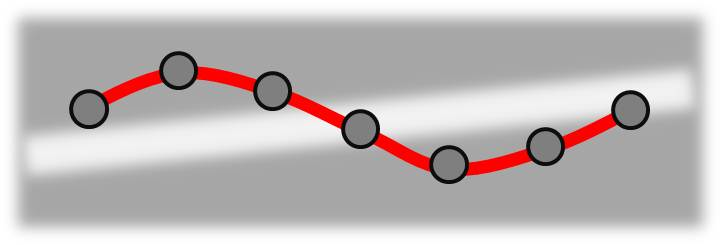
\includegraphics[width=0.44\textwidth]{figs/proc1.jpg}} \hspace{0.3cm}        
    \subfigure[]{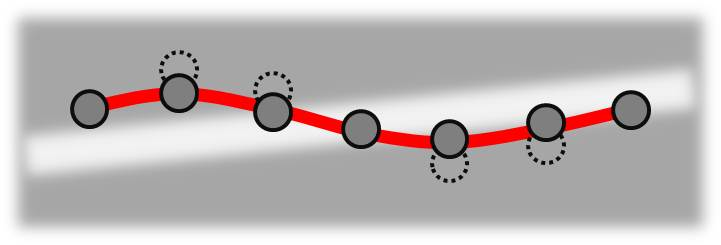
\includegraphics[width=0.44\textwidth]{figs/proc2.jpg}} \\
    \subfigure[]{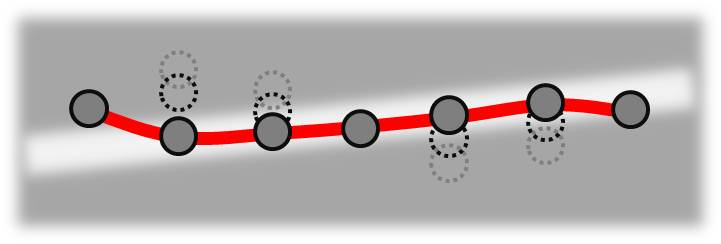
\includegraphics[width=0.44\textwidth]{figs/proc3.jpg}} \hspace{0.3cm} 
    \subfigure[]{\label{procSnakes4}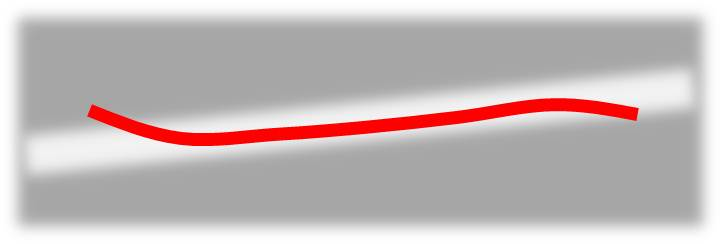
\includegraphics[width=0.44\textwidth]{figs/proc4.jpg}} 
    \caption{Avan�o da \emph{snake} com os pontos extremos fixos:(a) Curva inicial. (b) e (c) Avan�os intermedi�rios da curva. (d) Curva final.}
    \label{procSnakes}
\end{figure}

Em alguns casos, os pontos extremos da curva pode localizar-se distantes da regi�o de interesse, ocasionando o efeito ilustrado na Figura \ref{procSnakes4}, em que o posicionamento da aresta entre os v�rtices extremo e o interno mais pr�ximo pode tornar-se incoerente com a real posi��o da estrada. Desta forma, ap�s a aplica��o do m�todo, optou-se por excluir as arestas de liga��o com os extremos fixados no processo \emph{Snakes} (Figura \ref{verticeAresta}).
\begin{figure}[htb]
    \centering	   
    \subfigure[]{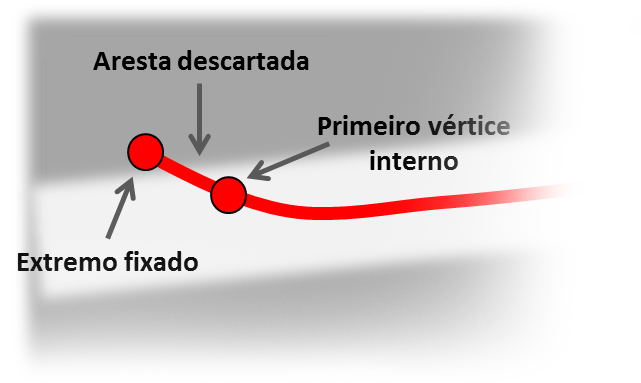
\includegraphics[width=0.64\textwidth]{figs/snakes.jpg}} \hspace{0.3cm}        
    \caption{Exclus�o da aresta de liga��o entre o extremo fixado e o v�rtice interno.}
    \label{verticeAresta}
\end{figure}

Na representa��o tradicional, a curva tende a ser atra�da para o contorno das formas, conforme as energias $E_{edge}$ e $E_{term}$. Sabendo-se que o operador deve obter os eixos de simetria, essas energias s�o inutilizadas, assim como o termo imposto pelo usu�rio $E_{con}$. Desta forma, o termo de energia externa $E_{ext}$, composta pelos fatores $E_{line}$, $E_{edge}$, $E_{term}$ e $E_{con}$, passa a ser composto somente pelo termo $E_{line}$, que consiste do produto entre a imagem suavizada e o fator de pondera��o $w_{line}$, o qual dependendo do sinal, definir� a atra��o da curva: negativo para perfis claros, e positivo para perfis escuros. Nessa defini��o, a curva ser� atra�da n�o para as fronteiras da estrada, mas sim para o seu centro.

Por ser uma imagem de radar, as estradas podem aparecer tanto em n�veis de cinza claros como escuros, e assim, o operador de extra��o deve ser capaz de reconhecer as duas caracter�sticas de tonalidade. O termo $E_{line}$, especifica qual caracter�stica que a curva dever� ser atra�da, ou seja, dependendo da sua sinaliza��o, negativo ou positivo, a curva ser� atra�da para fei��es escuras ou claras, respectivamente. 

Na Figura \ref{termoEnergiaExt}, s�o apresentados exemplos da aplica��o do operador de extra��o em um recorte na imagem de Paragominas-PA (ver Se��o \ref{secaoRadar}), cujas estradas aparecem em ambas representa��es, clara e escura. Na Figura \ref{termoEnergiaExt1} o termo de energia $E_{ext}$ possui sinal positivo, enquanto que na Figura \ref{termoEnergiaExt2}, o resultado apresentado possui o termo com sinal negativo. 
\begin{figure}[ht]\label{termoEnergiaExt}
    \centering	   
    \subfigure[]{\label{termoEnergiaExt1}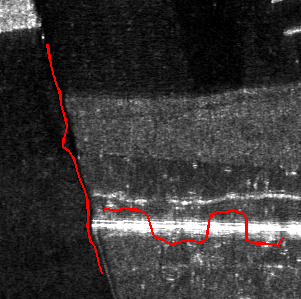
\includegraphics[width=0.42\textwidth]{figs/eExtPositivo.png}} \hspace{0.5cm}
    \subfigure[]{\label{termoEnergiaExt2}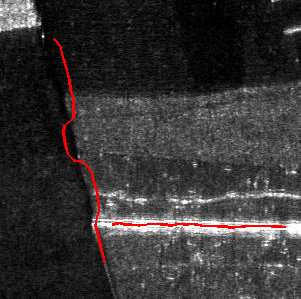
\includegraphics[width=0.42\textwidth]{figs/eExtNegativo.png}}     
    \caption{Resultados da extra��o para diferentes perfis de tonalidades: (a) Resultados obtidos com o termo de energia externa positivo e
    (b) Resultados obtidos com o termo de energia externa negativo.}    
\end{figure}

Nesta se��o, foram apresentados os conceitos envolvendo a utiliza��o do Modelo de Contorno Ativo na extra��o de estradas em imagens digitais. Com o objetivo de avaliar a efici�ncia do m�todo, ser�o apresentadas na se��o seguinte a m�trica de valida��o utilizada em muitos dos trabalhos envolvendo a extra��o de estradas.

\subsection{M�tricas de Qualidade}\label{metricas}
� essencial que, ap�s as etapas de processamento e aquisi��o dos resultados, seja medida a qualidade do m�todo aplicado. Isto permite visualizar se realmente o m�todo apresentado atingiu as expectativas para a resolu��o do problema. Geralmente, esta quantifica��o se baseia na compara��o entre o conjunto de estradas extra�das pelo m�todo e o conjunto-refer�ncia (verdade terrestre). A qualidade dos resultados � medida, respondendo-se a duas indaga��es: (i) Qu�o completa � a rede de estradas extra�das?; e (ii) Qu�o correta ela �? \cite{wiedemann2}. 

As medidas de qualidade n�o s�o destinadas a avaliar a extra��o e os resultados correspondentes de uma forma absoluta. Em vez disso, elas s�o utilizadas para comparar os resultados dos diferentes algoritmos \cite{heipke}. \citeonline{harvey}, \citeonline{wiedemann2}, \citeonline{heipke} e \citeonline{haupt} aplicaram t�cnicas semelhantes para a an�lise das fei��es extra�das pelo m�todo em quest�o. O conceito no qual se basearam � apresentado a seguir. 

Essencialmente, s�o definidos quatro fatores que representam cada resultado poss�vel que o extrator de estrada pode alcan�ar:
\begin{itemize}
 \item \textbf{TP (\emph{True Positive}):} O verdadeiro positivo representa as regi�es de estradas extra�das pelo m�todo que, por sua vez, 
					   pertence ao conjunto-refer�ncia.
 \item \textbf{TN (\emph{True Negative}):} O verdadeiro negativo representa as regi�es de n�o-estrada n�o extra�das pelo m�todo, que, 
					   por sua vez, pertence ao conjunto-refer�ncia.
 \item \textbf{FP (\emph{False Positive}):} O falso positivo representa as regi�es de estradas extra�das pelo m�todo que, por sua vez, n�o 
					    pertence ao conjunto-refer�ncia.
 \item \textbf{FN (\emph{False Negative}):} Por fim, o falso negativo representa as regi�es de estradas n�o extra�das pelo m�todo e que 
					   pertence ao conjunto-refer�ncia.
\end{itemize}

Com esses quatro fatores definidos, �ndices como corre��o, perfei��o, qualidade e redund�ncia, podem ser obtidos e, com
% diferen�a RMS (\emph{Root Mean Square}), 
isso, pode-se analisar a efici�ncia do m�todo. A seguir, descreve-se cada um desses �ndices e como s�o obtidos por meio dos fatores 
listados anteriormente.
\begin{itemize}
 \item Corre��o (\emph{Correctness}): O �ndice de corre��o representa a porcentagem de estradas extra�das corretamente, ou seja, a porcentagem de estradas que condiz com o conjunto-refer�ncia. \citeonline{wiedemann2} consideram um desvio-padr�o quando esses resultados s�o comparados. A Figura \ref{matchingPrinciple} ilustra esse princ�pio. 	
				      \begin{figure}[htb]
					  \centering	   
					  \subfigure[]{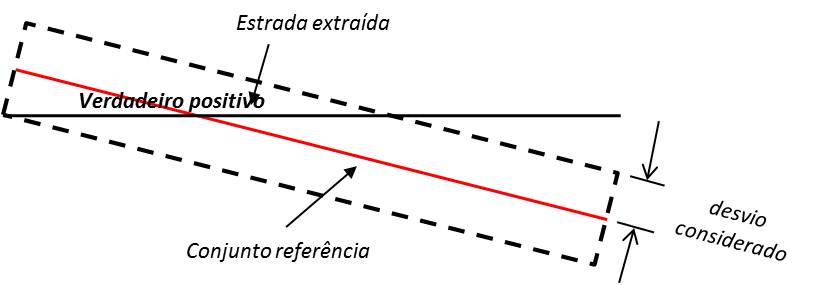
\includegraphics[width=0.47\textwidth]{figs/match1.jpg}} \hspace{0.1cm}        
					  \subfigure[]{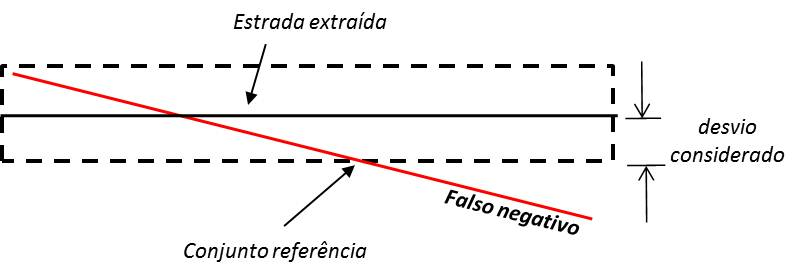
\includegraphics[width=0.47\textwidth]{figs/match2.jpg}} \\
					  \caption{Compara��o dos resultados extra�dos considerando um desvio-padr�o de erro: (a) Verdadeiro positivo. (b) Falso negativo.}\hspace{0.1cm}
					  \FONTE{Adaptado de \citeonline{wiedemann2}.}
					  \label{matchingPrinciple}
				      \end{figure}
				      A Equa��o \ref{correctnessEq} expressa o �ndice de corre��o.
				      \begin{align}\label{correctnessEq}
					corr &=\frac{exC}{ex}~, \notag \\
					corr &\approx \frac{TP}{TP+FP}~, \notag \\ 
					corr &\in [0;1]~, 
				      \end{align}
				      em que $exC$ � comprimento total dos segmentos extra�dos que coincidiram com a refer�ncia, e $ex$ � o comprimento total dos segmentos extra�dos. O valor �timo para o �ndice de corre��o � 1.
 \item Perfei��o (\emph{Completeness}): O �ndice de perfei��o representa a porcentagem em que os dados de refer�ncia coincidem com os dados de estradas extra�dos. Dado pela equa��o:
				      \begin{align}\label{completenessEq}
					perf &= \frac{rC}{r}~,\notag \\ 
					perf &\approx \frac{TP}{TP+FN}~, \notag \\ 
					perf &\in [0;1]~,
				      \end{align}	
				      em que $rC$ denota o comprimento total dos segmentos de refer�ncia que coincidiram com a extra��o, e $r$ o comprimento total dos segmentos de refer�ncia. O valor �timo para o �ndice de perfei��o � 1.
 \item Qualidade: A qualidade leva em conta tanto o �ndice de perfei��o dos dados extra�dos, como o �ndice de corre��o. � a medida mais geral entre todas elas e � expressa por: 
		  \begin{align}\label{qualityEq}
		    qualidade &= \frac{rC}{qq}~, \notag \\
		    qualidade &\approx \frac{TP}{TP+FP+FN}~, \notag \\ 
		    qualidade &\in [0;1]~,
		  \end{align}	
		  em que $qq$ denota a soma entre o comprimento total dos segmentos extra�dos que coincidiram com a refer�ncia e o comprimento total dos segmentos de refer�ncia que n�o coincidiram com a extra��o. O valor �timo para o �ndice de qualidade � 1.
 \item Redund�ncia: A redund�ncia representa a porcentagem em que foram extra�dos segmentos de reta redundantemente. A equa��o que calcula fator de redund�ncia � dada:
		       \begin{align}\label{RedundancyEq}
			 Redundancia &= \frac{rr}{ex}~, \notag \\ 
% 			 Redundancia &\approx \frac{TP + FN - ref}{TP}~,\notag \\ 
			 Redundancia &\in [0;+\infty]~, 
		       \end{align}
			em que $rr$ denota a diferen�a entre o comprimento total dos segmentos extra�dos que coincidiram com a refer�ncia e o comprimento total dos segmentos de refer�ncia que coincidiram com a extra��o. %E $ref$, o tamanho do conjunto refer�ncia. 
			O valor �timo para o fator de redund�ncia � 0.
%   \item Diferen�a RMS: A diferen�a RMS representa a dist�ncia m�dia entre as fei��es extra�das pelo m�todo e as fei��es presentes no 
% 		       conjunto refer�ncia. Quando � considerado um valor de desvio, como apresentado por Wiedemann et al. \citeonline{wiedemann2}),
% 		       a diferen�a RMS depender� exclusivamente deste valor. A equa��o que calcula a diferen�a RMS � dada por:
% 		       \begin{align}\label{differenceRMSEq}
% 			 RMS &= \sqrt{\frac{\sum^l_{i=1}(d(extr_i;ref)^2)}{l}} \\ \notag
% 			 RMS &\in [0;desvio] 
% 		       \end{align}	
% 		       em que $l$ � o n�mero de segmentos de reta extra�dos que coincidirem com o conjunto refer�ncia. $d(extr_i;ref)$ � a menor dist�ncia entre o 
% 		       i�simo segmento de reta em rela��o ao i�simo segmento de reta correspondente no conjunto refer�ncia. O valor �timo para 
% 		       o �ndice da diferen�a RMS � 0.
\end{itemize}

% Assim como \citeonline{wiedemann2} consideraram o desvio tanto para o conjunto refer�ncia como para o conjunto extra�do, ilustrado na Figura \ref{matchingPrinciple}, sendo 
% este desvio um valor fixo para ambos. O desvio utilizado por \citeonline{wiedemann2} n�o � adotado na valida��o do m�todo de extra��o deste trabalho. Ao inv�s disso, 
% o desvio no conjunto refer�ncia fica sendo a pr�pria largura da estrada em quest�o, em que a largura de cada segmento de reta � definida na imagem 
% refer�ncia, utilizada para a valida��o do resultado. Por outro lado, o segmento de reta extra�do � caracterizado por uma linha de largura de 1 \emph{pixel}, correspondendo 
% ao eixo de simetria da estrada, que, ao ser extra�da, � a �nica caracter�stica conhecida. No entanto, na valida��o dos resultados � essencial que os segmentos de reta 
% extra�dos possuam o mesmo desvio agregado aos respectivos segmentos de reta no conjunto refer�ncia. Como a largura da estrada no conjunto extra�do � desconhecida, o desvio 
% agregado ao conjunto extra�do � a largura predominante das estradas presentes na cena, informa��o fornecida pelo usu�rio.
 
Assim como \citeonline{wiedemann2} consideraram o desvio tanto para o conjunto refer�ncia como para o conjunto extra�do, ilustrado na Figura \ref{matchingPrinciple}, sendo este desvio um valor fixo para ambos. O desvio utilizado por \citeonline{wiedemann2} n�o � adotado na valida��o do m�todo de extra��o deste trabalho. Ao inv�s disso, o conjunto refer�ncia utilizado constitui-se dos eixos centrais de largura de 1 \emph{pixel}, constru�dos a partir da refer�ncia cartogr�fica. Tais eixos s�o dilatados de acordo com a largura de estrada predominante na cena. O segmento de reta extra�do, por sua vez, � tamb�m caracterizado por uma linha de largura de 1 \emph{pixel}, 
correspondendo ao eixo de simetria da estrada, que, ao ser extra�da, � a �nica caracter�stica conhecida. No entanto, na valida��o dos resultados � essencial que os segmentos de reta extra�dos possuam o mesmo desvio agregado aos respectivos segmentos de reta no conjunto refer�ncia. Como a largura da estrada no conjunto extra�do � desconhecida, o desvio agregado ao conjunto extra�do � a largura predominante das estradas presentes na cena, a mesma agregada na dilata��o do conjunto refer�ncia.

% Uma outra alternativa para a visualiza��o dos �ndices de qualidade, e talvez uma maneira mais n�tida de an�lise, � a plotagem da Curva de Caracter�sticas de Opera��o do Receptor (\emph{Receiver Operating Characteristic - ROC}) para a visualiza��o da sensibilidade dos resultados, que implica no cruzamento das taxas TP e FP. A se��o seguinte detalha como a curva � obtida a partir destes valores.

% \subsection{Curva de Caracter�sticas de Opera��o do Receptor (\emph{Receiver Operating Characteristic - ROC})}\label{ROCsection}
% A Curva de Caracter�sticas de Opera��o do Receptor, em ingl�s \emph{Receiver Operating Characteristic}, ou simplesmente curva ROC, foi 
% desenvolvida inicialmente no campo de decis�o estat�stica e, posteriormente, utilizada para a an�lise de sinais de radares durante a Segunda 
% Guerra Mundial \cite{collison}. Tinha como principal objetivo avaliar a rela��o entre o sinal e o ru�do proveniente de radares a�reos, at� ent�o 
% chamados de operadores de recep��o (\emph{receiver operator}). Sua utiliza��o tornava poss�vel a distin��o entre alvos inimigos, aliados e 
% ru�dos de transmiss�o. 
% 
% Para \citeonline{fawcett}, a curva ROC � uma t�cnica para a visualiza��o, organiza��o e de sele��o de classificadores baseando-se em seu desempenho, cuja
% t�cnica t�m sido muito utilizada na teoria de detec��o de sinais para descrever o equil�brio entre taxas de falso alarme de classificadores. Na comunidade 
% m�dica cient�fica, h� uma literatura extensa envolvendo o uso de gr�ficos ROC para testes de diagn�sticos. Na biomedicina, a t�cnica � extensivamente 
% utilizada para avaliar a efic�cia de diagn�sticos entre indiv�duos saud�veis e doentes \cite{metz}. O conceito se estendeu para a an�lise de m�todos 
% de extra��o de estradas como forma de mensurar o desempenho dos mesmos. 
% \begin{figure}[htb]
%     \centering	   
%     \subfigure[]{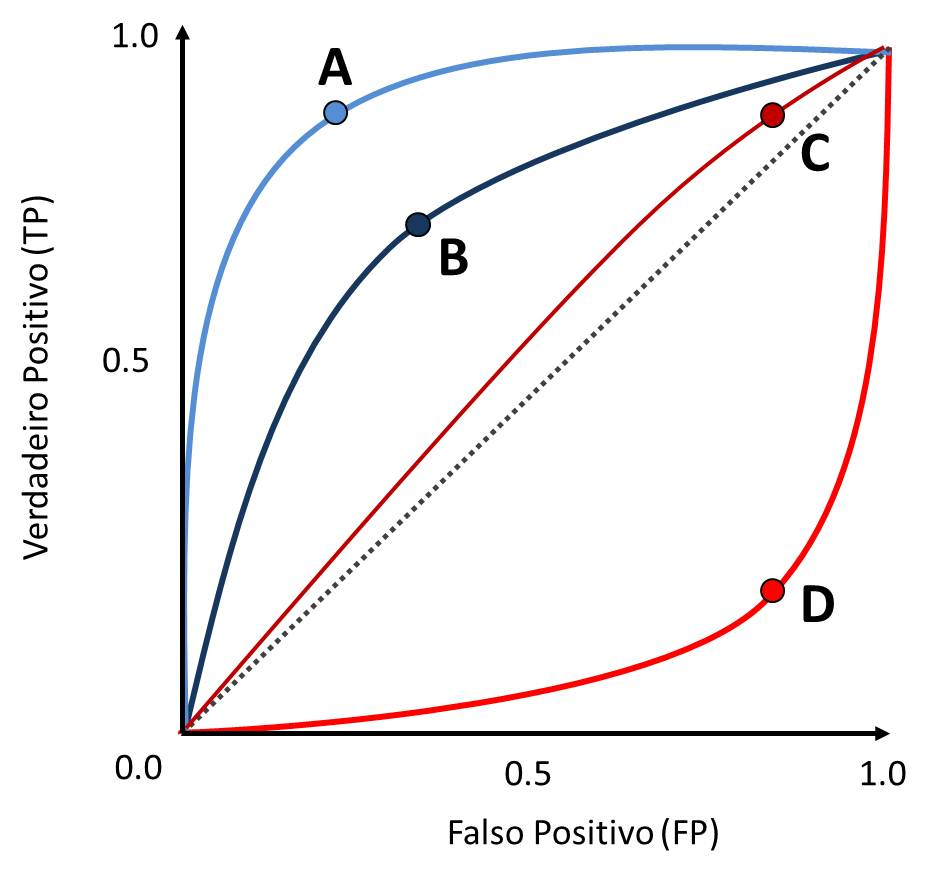
\includegraphics[width=0.44\textwidth]{figs/curvaROC.jpg}} \hspace{0.1cm}        
%     \caption{Exemplo de plotagem da curva ROC para quatro experimentos (A, B, C e D).}
%     \label{curvaROC}
% \end{figure}
% 
% A curva � representada basicamente pelas taxas de verdadeiros positivos (TP) e falsos positivos (FP), associadas no gr�fico a seus 
% respectivos n�veis. A Figura \ref{curvaROC} ilustra um exemplo de como seria a curva ROC para alguns exemplos de TP em rela��o a FP. 
% A linha descont�nua no centro do gr�fico denota o indicador de baixa efetividade, pois uma vez que o resultado tenha apresentado um alto 
% �ndice de acerto (eixo TP), apresentou tamb�m um alto �ndice de erros (eixo FP). Sendo assim, fica evidente que, no caso de bons resultados, 
% ser�o plotadas curvas acima desse indicador. O ponto \textbf{A} identifica a curva confeccionada pelos valores da primeira linha na Tabela 
% \ref{tabela1}, representando neste caso o experimento com o melhor resultado, tendo em vista o elevado �ndice de acerto (TP) em contraposi��o 
% com � baixa taxa de erros (FP). O ponto \textbf{B} ainda pode ser considerado como um resultado satisfat�rio, pois apresentou uma taxa de 
% erro menor que $0,6$, al�m, de ter apresentado um valor satisfat�rio de acertos. J� os pontos \textbf{C} e \textbf{D} n�o s�o considerados 
% como bons resultados. Embora \textbf{C} tenha se comportado acima do indicador de baixa efetividade, a curva apresentou-se pr�xima a ele, o que indica
% um resultado incerto. Por fim, fica evidente que a curva \textbf{D} apresentou m� qualidade em vista de se situar abaixo do indicador de 
% efetividade. Desta maneira, analisar qu�o eficiente determinado experimento se mostrou em rela��o aos demais torna-se uma tarefa 
% simples.
% \begin{table}[!ht]
% \begin{center}
% \caption{Resultados demonstrativos para diferentes experimentos de extra��o.}
% \begin{tabular}{l||c|c}\label{tabela1}
% Experimentos & TP & FP\\ \hline \hline
% \textbf{A} & $0,88$ & $0,26$\\
% \textbf{B} & $0,75$ & $0,43$\\
% \textbf{C} & $0,87$ & $0,84$\\
% \textbf{D} & $0,23$ & $0,82$
% \end{tabular}
% \end{center} 
% \end{table}
% 
% Assim como as m�tricas de qualidade apresentadas por \citeonline{wiedemann2}, a curva ROC tamb�m ser� utilizada neste trabalho 
% como ferramenta para a an�lise do m�todo de extra��o de estradas. 

Este cap�tulo apresentou os conceitos e a estrat�gia envolvendo a solu��o do problema de extra��o de estradas em imagens digitais, 
bem como as medidas de desempenho do m�todo. A valida��o dos resultados seguem as medidas apresentadas na �ltima se��o deste cap�tulo, tanto
para dados sint�ticos como para imagens SAR. %% 3o capitulo
\chapter{RESULTADOS E DISCUSS�O}\label{capResultados}
Neste cap�tulo, s�o apresentados os resultados dos testes realizados para avaliar o desempenho do m�todo de extra��o de estradas em imagens digitais desenvolvido e apresentado no cap�tulo anterior. As se��es foram categorizadas de acordo com os diferentes experimentos realizados. Em raz�o da qualidade das imagens e tamb�m para efeitos de an�lise, os experimentos s�o realizados primeiramente sobre dados sint�ticos e, posteriormente, sobre dados de radar. Sendo assim, a primeira parte deste cap�tulo consiste em apresentar os dados utilizados nos experimentos: imagens sint�ticas (Se��o \ref{secaoSint}) e imagens reais de radar (Se��o \ref{secaoRadar}). Na Se��o \ref{SecaoResultados} s�o apresentadas a avalia��o e discuss�o envolvendo os resultados, as medidas obtidas, tempos de processamento e complexidade do m�todo.

% A avalia��o de desempenho � realizada considerando-se duas imagens, a do resultado obtido e a do resultado desejado. Essas duas informa��es s�o ent�o 
% contrastadas e, assim, s�o obtidos os par�metros apresentados na Se��o \ref{metricas}, que, em seguida, s�o plotados na curva ROC.
 
% Al�m da avalia��o realizada sobre as medidas de valida��o, � realizado tamb�m a an�lise que considera os resultados de diferentes trabalhos 
% envolvendo a extra��o de estradas em imagens de radar. Nessa an�lise, n�o s�o considerados somente os trabalhos abordando as t�cnicas 
% apresentadas aqui, mas sim, os trabalhos que abordaram o conceito de extra��o de estradas em imagens de radar e utilizaram outras t�cnicas 
% para a resolu��o do problema. Por ser grande o n�mero de trabalhos que aborda o tema, foram selecionados os principais trabalhos que aplicaram 
% a mesma m�trica de valida��o, para que assim, fossem feitas as respectivas compara��es.

\section{Dados Sint�ticos}\label{secaoSint}
As imagens sint�ticas empregadas neste trabalho possuem tamanhos pr�-determinados de 574$\times$574 \emph{pixels} (linhas$\times$colunas) e foram simuladas visando o problema da extra��o de estradas. O processo de obten��o das imagens sint�ticas envolvem tr�s etapas: cria��o, classifica��o das regi�es e modelagem estat�stica \cite{santanna}. O resultado das duas etapas iniciais denomina-se imagem \emph{phantom} (imagem idealizada de classes de homogeneidade) \cite{scofield}. Ser�o utilizadas tr�s imagens sint�ticas para os experimentos. As imagens, todas em alto contraste, s�o diferenciadas apenas em suas propriedades polarim�tricas, deste modo, as caracter�sticas espectrais das estradas presentes nas diferentes imagens s�o modificadas. 

Na se��o seguinte, s�o apresentados os detalhes da obten��o da imagem \emph{phantom}, imagem simulada a partir de dados reais.

\subsection{Obten��o do \emph{Phantom}}
A imagem \emph{phantom} possui dimens�es de 574$\times$574 \emph{pixels}, representando uma regi�o contendo estradas (�reas claras) orientadas em dire��es distintas. As estradas presentes na cena possuem largura de 3 e 15 \emph{pixels}, respectivamente. Portanto, a imagem \emph{phantom} que ser� utilizada como imagem de verdade terrestre (imagem refer�ncia), possui apenas 2 classes: estrada (regi�es de estrada na imagem) e fundo (regi�es que n�o s�o estradas). 

As imagens sint�ticas geradas s�o polarim�tricas, nas polariza��es HH, HV e VV, e em uma visada (1-\emph{look}). As matrizes de covari�ncia das duas classes da imagem utilizadas para a simula��o das imagens sint�ticas foram extra�das a partir de uma imagem SAR polarim�trica, banda L (1,27GHz), adquirida em outubro de 2005 pelo sensor R99B, da For�a A�rea Brasileira da regi�o do munic�pio de Paul�nea, no estado de S�o Paulo (Figura \ref{RefPhantom}). 
\begin{figure}[htb]\label{RefPhantom}
    \centering	   
    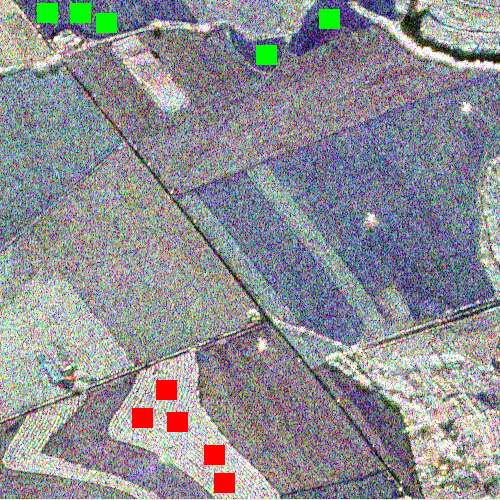
\includegraphics[width=0.50\textwidth]{figs/amostras.png}
    \caption{Imagem SAR da regi�o de Paul�nea-SP e respectivas amostras para as classes estrada e fundo. Imagem em composi��o colorida HH(R), HV(G) e VV(B).}       
\end{figure}
As amostras possuem dimens�es de 20$\times$20 \emph{pixels}. Para cada classe (estrada e fundo) foram extra�das 5 amostras, utilizadas para estimar a matriz de covari�ncia de cada uma das classes. As matrizes de covari�ncia complexas das classes estrada e fundo � dada, respectivamente, por:
\begin{center}
$\sum_{estrada} = 
\begin{pmatrix}
   (0,0129;0,0000) & (0,0012;-0,0007) & (0,0039;0,0019) \\ (0,0012;0,0007) & (0,0337;0,0000) & (-0,0008;-0,0012) \\ (0,0039;-0,0019) & (-0,0008;0,0012) & (0,0154;0,0000)
 \end{pmatrix}
$

$\sum_{fundo} = 
 \begin{pmatrix}
  (0,0219;0,0000) & (-0,0066;-0,0009) & (0,0031;-0,0048) \\ (-0,0066;0,0009) & (0,0020;0,0000) & (-0,0007;0,0016) \\ (0,0031;0,0048) & (-0,0007;-0,0016) & (0,0015;0,0000)
 \end{pmatrix}
$
\end{center}
Os elementos s�o baseados na nota��o ($\Re,\Im$), em que $\Re$ representa a parte real do n�mero complexo e $\Im$ a parte imagin�ria. A metodologia empregada para a obten��o da imagem \emph{phantom} (dado simulado) � detalhada por \citeonline{santanna}. A imagem \emph{phantom} empregada bem como as imagens simuladas, s�o apresentadas na Figura \ref{sinteticas}.

\begin{figure}[!htb]
    \centering	   
    \subfigure[]{\label{recortePhantom}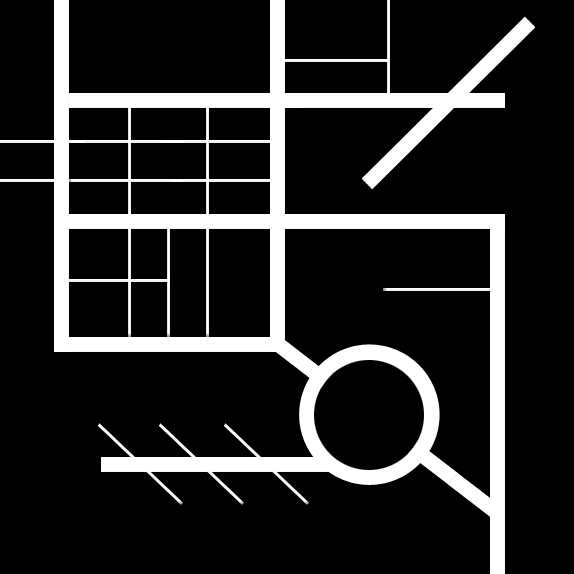
\includegraphics[width=0.40\textwidth]{figs/sintetica1.jpg}} \hspace{0.5cm}
    \subfigure[]{\label{recortesintetico1a}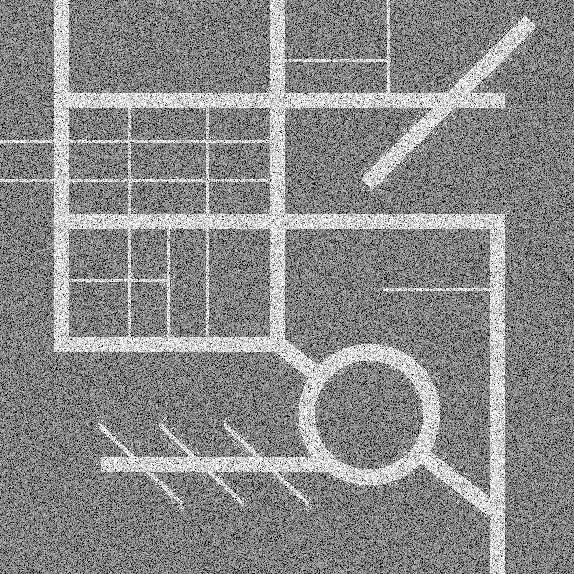
\includegraphics[width=0.40\textwidth]{figs/ImagPolvv_HC.jpg}} \\     
    \subfigure[]{\label{recortesintetico1b}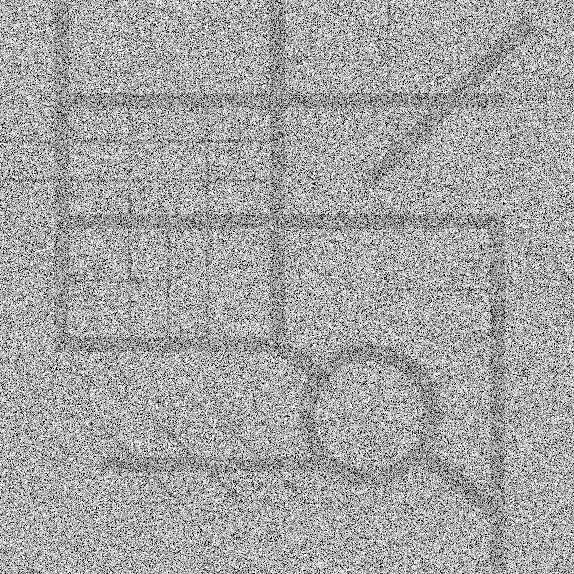
\includegraphics[width=0.40\textwidth]{figs/ImagPolhh_HC.jpg}} \hspace{0.5cm}
    \subfigure[]{\label{recortesintetico1c}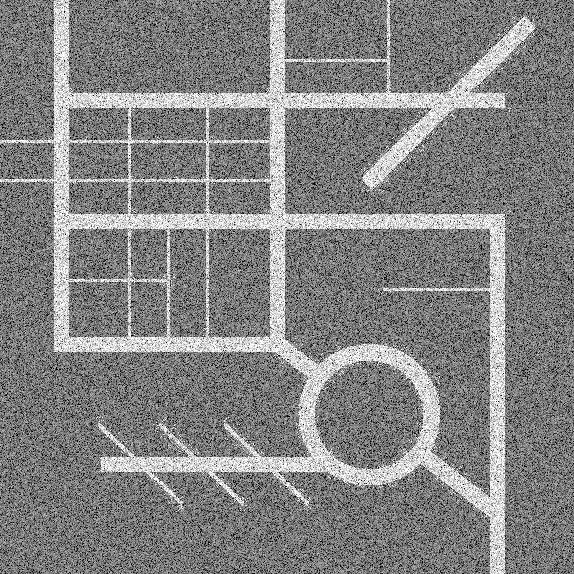
\includegraphics[width=0.40\textwidth]{figs/ImagPolhv_HC.jpg}}
    \caption{Imagens sint�ticas de radar: (a) \emph{Phantom} (b) Polariza��o VV. (c) Polariza��o HH. (d) Polariza��o HV.}     
    \label{sinteticas}
\end{figure}

\section{Dados de SAR}\label{secaoRadar}
Para a realiza��o dos experimentos foram adotados cinco diferentes recortes de uma imagem SAR com dimens�es 513$\times$513, 434$\times$573, 247$\times$707, 460$\times$649 e 357$\times$357 \emph{pixels}, respectivamente. Os recortes recobrem a regi�o de Paragominas no estado do Par�, com resolu��o radiom�trica de 8 \emph{bits} e espacial de 2,5 metros na banda P e polariza��o HH. A imagem foi adquirida com o sensor OrbiSAR da empresa Orbisat da Amaz�nia Ind. e Aerolevantamento S.A. no per�odo de aerolevantamento entre 11 de fevereiro de 2007 e 13 de mar�o de 2007, com altitude de voo em torno de $11.000$ metros. Esta imagem � mostrada na Figura \ref{paragominasTotal}, em que s�o ressaltadas as cinco regi�es que representam os recortes extra�dos para a realiza��o dos experimentos.
\begin{figure}[!htb]
    \centering	       
    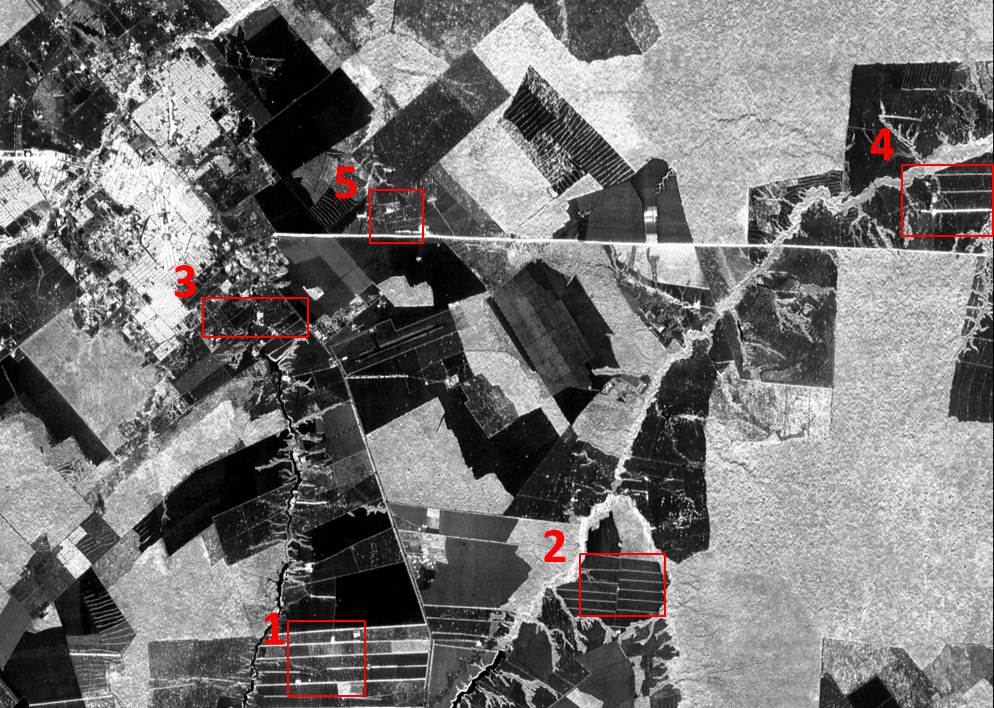
\includegraphics[width=0.90\textwidth]{figs/recortesParagominas.jpg}\\     
    \caption{Imagem SAR da regi�o de Paragominas-PA e as localiza��es das �reas de estudo.}      
    \label{paragominasTotal} 
\end{figure}

Todos os recortes s�o baseados em regi�es n�o urbanizadas. Na Figura \ref{recorte1} � ilustrado o recorte da regi�o 1 (recorte 1) e a sua respectiva refer�ncia cartogr�fica, a qual ser� utilizada como verdade terrestre na localiza��o das estradas. As estradas na Figura \ref{recorte1b} est�o representadas por linhas tracejadas. Pode-se observar, ainda, que h� um predom�nio das estradas orientadas na dire��o horizontal, as quais aparecem na 
imagem (Figura \ref{recorte1a}) em n�veis de cinza mais claros que o n�vel de cinza do fundo e tamb�m apresentam largura maior que as estradas orientadas em outras dire��es. A classe fundo por apresentar alta variabilidade de n�veis de cinza pode dificultar a tarefa de extra��o de estradas.
% As refer�ncias cartogr�ficas apresentadas nessa se��o, constituem-se do resultado da interpreta��o visual realizada por uma equipe de 
%profissionais, esta por sua vez, pertencentes a empresa Orbisat, acima citada.
\begin{figure}[!htb]
    \centering	   
    \subfigure[]{\label{recorte1a}\includegraphics[width=0.42\textwidth]{figs/recorte1.png}} \hspace{0.5cm}
    \subfigure[]{\label{recorte1b}\includegraphics[width=0.40\textwidth]{figs/ref.png}} 
    %\subfigure[]{\label{recorte1c}\includegraphics[width=0.42\textwidth]{figs/ref_estradas_recorte1.jpg}}   
    \caption{Recorte 1: (a) Imagem SAR (513$\times$513 \emph{pixels}). (b) Refer�ncia cartogr�fica.}
    \FONTE{\citeonline{orbisat}.}
    \label{recorte1}
\end{figure}

O recorte 2, mostrado na Figura \ref{recorte2a}, apresenta estradas em n�veis de cinza claros, estreitas (aproximadamente 7 \emph{pixels}) e entorno escuro. As linhas tracejadas e cont�nuas vermelhas, expressas na refer�ncia cartogr�fica (Figura \ref{recorte2b}), representam as estradas na imagem. Assim como no recorte 1 (Figura \ref{recorte1}), as estradas com orienta��o horizontal s�o predominantes no recorte 2, sendo essas interceptadas por somente uma estrada de orienta��o pr�xima � vertical, na qual � caracterizada por n�veis de cinza mais escuros em rela��o ao seu entorno. A classe fundo, entretanto, � aparentemente mais homog�nea que a classe fundo apresentada no recorte 1, o que pode favorecer o m�todo de extra��o. No entanto, as estradas no recorte 2 apresentam larguras menores, devido essa caracter�stica, o m�todo pode confundi-las com seu entorno.
\begin{figure}[!htb]
    \centering	   
    \subfigure[]{\label{recorte2a}\includegraphics[width=0.47\textwidth]{figs/recorte2.png}} \hspace{0.2cm}
    \subfigure[]{\label{recorte2b}\includegraphics[width=0.47\textwidth]{figs/ref_recorte2.jpg}} 
    %\subfigure[]{\label{recorte2c}\includegraphics[width=0.47\textwidth]{figs/ref_estradas_recorte2.jpg}}    
    \caption{Recorte 2: (a) Imagem SAR (434$\times$573 \emph{pixels}). (b) Refer�ncia cartogr�fica.}   
    \FONTE{\citeonline{orbisat}.}
    \label{recorte2}
\end{figure}

O terceiro recorte, ilustrado na Figura \ref{recorte3}, apresenta uma complexidade maior em rela��o aos anteriores. As linhas tracejadas e cont�nuas vermelhas presentes na Figura \ref{recorte3b}, representam as estradas e caminhos a serem extra�dos pelo m�todo de extra��o. Todas as estradas presentes na cena s�o orientadas na dire��o diagonal, as quais aparecem na Figura \ref{recorte3b} em n�veis de cinza claro e largura variando entre 1 a 3 \emph{pixels}. A classe fundo apresenta alta variabilidade de n�veis de cinza. A presen�a de edifica��es, lagos e rios pode tornar confuso a classifica��o, principalmente no processo de semea��o.
\begin{figure}[!htb]
    \centering	   
    \subfigure[]{\label{recorte3a}\includegraphics[width=0.73\textwidth]{figs/recorte3.png}} 
    \subfigure[]{\label{recorte3b}\includegraphics[width=0.73\textwidth]{figs/ref_recorte3.jpg}} 
    %\subfigure[]{\label{recorte3c}\includegraphics[width=0.73\textwidth]{figs/ref_estradas_recorte3.jpg}}    
    \caption{Recorte 3: (a) Imagem SAR (247$\times$707 \emph{pixels}). (b) Refer�ncia cartogr�fica.}  
    \FONTE{\citeonline{orbisat}.}
    \label{recorte3}  
\end{figure}
As caracter�sticas de superf�cie de rio ou lago fazem com que, quase sempre, o retorno do sinal transmitido tenha baixa intensidade, tornando estas regi�es escuras. Devido � n�o-constru��o de uma heur�stica que certifique que tal regi�o n�o � uma estrada e considerando que algumas estradas possuem caracter�sticas tais que tornam sua representa��o mais escura na imagem de radar, a probabilidade do m�todo de extra��o reconhecer um lago como uma estrada � grande.

Na Figura \ref{recorte4} � mostrada a regi�o 4 (recorte 4), em que grande parte das estradas presentes na cena aparecem em n�veis de cinza claros, caracterizadas pelas linhas tracejadas e cont�nuas vermelhas na Figura \ref{recorte4b}. Assim como na Figura \ref{recorte3}, a classe fundo apresenta tamb�m um grande variabilidade de n�veis de cinza, causado pela presen�a de edifica��es, lagos e regi�es de mata ciliar. As estradas s�o orientadas tanto na dire��o horizontal como na vertical, em larguras que variam entre 3 a 15 \emph{pixels}.
\begin{figure}[!htb]
    \centering	   
    \subfigure[]{\label{recorte4a}\includegraphics[width=0.45\textwidth]{figs/recorte4.png}} \hspace{0.2cm}
    \subfigure[]{\label{recorte4b}\includegraphics[width=0.45\textwidth]{figs/ref_recorte4.jpg}} 
    %\subfigure[]{\label{recorte3c}\includegraphics[width=0.73\textwidth]{figs/ref_estradas_recorte3.jpg}}    
    \caption{Recorte 4: (a) Imagem SAR (460$\times$649 \emph{pixels}). (b) Refer�ncia cartogr�fica.}  
    \FONTE{\citeonline{orbisat}.}
    \label{recorte4}  
\end{figure}

Por fim, na Figura \ref{recorte5}, � ilustrado o recorte 5. As estradas neste recorte aparecem em n�veis de cinza mais claros que seu entorno, grande parte delas, aparecendo em larguras entre 1 e 2 \emph{pixels}. As linhas tracejadas identificam as estradas com larguras inferiores a 2 \emph{pixels}, e a linha cont�nua vermelha a estrada com largura aproximada de 12 \emph{pixels}. Nesta regi�o, a varia��o de n�veis de cinza da classe fundo pode ser classificada como moderada, contudo, os perfis de estrada com larguras inferiores podem dificultar o processo de extra��o.
\begin{figure}[!htb]
    \centering	   
    \subfigure[]{\label{recorte5a}\includegraphics[width=0.40\textwidth]{figs/recorte5.jpg}} \hspace{0.3cm}
    \subfigure[]{\label{recorte5b}\includegraphics[width=0.40\textwidth]{figs/ref_recorte5.jpg}} 
    %\subfigure[]{\label{recorte3c}\includegraphics[width=0.73\textwidth]{figs/ref_estradas_recorte3.jpg}}    
    \caption{Recorte 5: (a) Imagem SAR (357$\times$357 \emph{pixels}). (b) Refer�ncia cartogr�fica.}  
    \FONTE{\citeonline{orbisat}.}
    \label{recorte5}  
\end{figure}

As regi�es 1 e 2 (Figuras \ref{recorte1} e \ref{recorte2}) representam regi�es menos complexas para o m�todo de extra��o. Tendo em vista a aus�ncia de �reas heterog�neas, tais recortes apresentam estradas mais evidentes, sem grande interfer�ncia de ru�do ou alta variabilidade de n�veis de cinza em seu entorno. No entanto, as demais regi�es podem apresentar um grau elevado de complexidade, tal como aquelas regi�es cuja estradas n�o aparecem nitidamente, ou aparecem em larguras muito inferiores, o que pode aumentar a margem de erro do m�todo de semea��o. A presen�a de outros objetos n�o pertencentes � classe estrada, tais como rios, lagos, matas e edifica��es, podem contribuir consideravelmente com o mau desempenho do m�todo. 

Na pr�xima se��o, s�o apresentados os resultados obtidos, bem como a an�lise de desempenho do m�todo utilizando as imagens apresentadas nesta se��o.

\section{Resultados e Valida��o}\label{SecaoResultados}
% No princ�pio b�sico de uma RNA, � exigido a apresenta��o de um conjunto de informa��es ou padr�es de treinamento, tal que a rede se adapte a fim de 
% reconhecer essas informa��es em uma aplica��o futura. Uma vez que os padr�es de treinamento utilizados neste trabalho s�o baseados nas informa��es 
% presentes nas imagens de radar, os padr�es presentes nas imagens sint�ticas n�o s�o reconhecidos eficientemente pelo m�todo. 
A fim de avaliar a efici�ncia do m�todo \emph{Snakes}, os pontos-sementes nas imagens sint�ticas s�o selecionados manualmente, de forma que a localiza��o desses pontos seja realizada adequadamente pr�ximos �s fei��es e, assim, a an�lise do extrator � voltada apenas para o comportamento do m�todo \emph{Snakes}. As medidas de desempenho s�o baseadas no m�todo desenvolvido por \citeonline{wiedemann2}.

% ------------ IMAGEM SINT�TICA -----------------------------------------------------------------------------------------------------------
O primeiro experimento � realizado sobre a imagem sint�tica 1 de polariza��o VV, apresentada na Figura \ref{recortesintetico1a}. As fei��es presentes na imagem, aparecem em larguras de 3 e 15 \emph{pixels}, em n�veis de cinza mais claro que a classe fundo. Em raz�o das estradas neste experimento serem mais evidentes e os pontos-sementes serem selecionados adequadamente por um m�todo, a aplica��o do m�todo \emph{Snakes} foi favorecida. Os resultados da aplica��o do m�todo de extra��o s�o mostrados na Figura \ref{sintetica2Snakes}.
\begin{figure}[!htbl]
    \centering	   
    \subfigure[]{\label{sintetica2a}\includegraphics[width=0.47\textwidth]{figs/FinalResults/ResultsSinteticas/result_seeding_sinthetic1_image.jpg}} \hspace{0.5cm}
    \subfigure[]{\label{sintetica2b}\includegraphics[width=0.47\textwidth]{figs/FinalResults/ResultsSinteticas/result_snake_sinthetic1_image.jpg}} 
    \caption{Resultados obtidos para a imagem sint�tica 1 (Figura \ref{recortesintetico1a}): (a) Pontos-sementes selecionados manualmente e
     (b) Resultado final ap�s a aplica��o do m�todo \emph{Snakes}.}
    \label{sintetica2Snakes}
\end{figure}

Em alguns trechos da curva n�o ocorre a convers�o para o eixo central da via, isso ocorre devido ao n�mero de itera��es n�o serem suficiente para o processo de minimiza��o. Contudo, a efici�ncia do m�todo para a extra��o do eixo de simetria em ambas as larguras de estrada (3 e 15 \emph{pixels}), mostrou-se satisfat�ria. Na Tabela \ref{validacaoSintetica1} s�o apresentados os valores adquiridos com a valida��o dos resultados apresentados na Figura 
\ref{sintetica2Snakes}.
\begin{table}[!ht]
\renewcommand{\arraystretch}{1.}\addtolength{\tabcolsep}{4pt}
\begin{center}
\small
\tabcolsep 2.9pt
\caption{Medidas de desempenho do m�todo sobre a Figura \ref{recortesintetico1a}.}
\begin{tabular}{l||cccc}
\hline
& \textbf{Perfei��o} & \textbf{Corre��o} & \textbf{Qualidade} & \textbf{Redund�ncia}\\ \hline \hline 
\textbf{Sint�tica 1} & $0,77$ & $0,63$ & $0,71$ & $0,02$ \\ \hline
\end{tabular}
\label{validacaoSintetica1}
\end{center} 
\end{table} 

Uma vez que a semea��o � realizada manualmente e os pontos-sementes selecionados sempre pr�ximos �s fei��es, � esperado que os fatores de perfei��o, corre��o e redund�ncia mantenha-se elevados, pois, a medida de perfei��o diz respeito � porcentagem que conjunto extra�do sobrep�s o conjunto refer�ncia, a corre��o, a porcentagem que o conjunto refer�ncia sobrep�s o conjunto extra�do, e a medida de redund�ncia, a porcentagem que os segmentos de reta pertencentes ao conjunto extra�do sobrep�s uns aos outros. Sabendo que a semea��o � realizada pr�xima �s fei��es, e considerando a convers�o esperada do m�todo \emph{Snakes}, o conjunto extra�do se manter� pr�ximo dos eixos centrais, ou seja, medida de perfei��o elevada, e consequentemente, medida de corre��o tamb�m elevada, pois nenhum ponto-semente foi selecionado distante das fei��es. O fator redund�ncia �, portanto, tamb�m elevado, pois para uma �nica fei��o � semeada um �nico conjunto de pontos, o que, quase sempre, exclui a possibilidade de sobreposi��es.

No segundo experimento, o m�todo \emph{Snakes} � aplicado sobre a imagem sint�tica 2 de polariza��o HH (Figura \ref{recortesintetico1b}). As estradas, principalmente as de largura inferior, confundem-se quase que inteiramente com a classe fundo, tornando dif�cil a tarefa de reconhecimento. No entanto, as curvas convergiram com exatid�o para o centro das vias em muito dos trechos dos segmentos de reta. O sinal do par�metro $w_{line}$, que considera o tipo de perfil de estrada que a curva deve ser atra�da, deve ser alterado. Considerando que as estradas na Figura \ref{recortesintetico1b} apresentam tonalidades mais escura que a classe fundo, � agregado o sinal positivo ao par�metro $w_{line}$, que possibilita � curva atrair-se para o centro de fei��es escuras.

Os experimentos realizados sobre a imagem sint�tica da Figura \ref{recortesintetico1b} s�o apresentados na Figura \ref{sintetica1Snakes}.
\begin{figure}[!htbl]
    \centering	   
    \subfigure[]{\label{sintetica1a}\includegraphics[width=0.47\textwidth]{figs/FinalResults/ResultsSinteticas/result_seeding_sinthetic2_image.jpg}} \hspace{0.5cm}
    \subfigure[]{\label{sintetica1b}\includegraphics[width=0.47\textwidth]{figs/FinalResults/ResultsSinteticas/result_snake_sinthetic2_image.jpg}} 
    \caption{Resultados obtidos para a imagem sint�tica 2 (Figura \ref{recortesintetico1b}): (a) Pontos-sementes selecionados manualmente e
     (b) Resultado final ap�s a aplica��o do m�todo \emph{Snakes}.}
    \label{sintetica1Snakes}
\end{figure}

A aplica��o do m�todo \emph{Snakes} mostrou-se eficiente ao identificar, em grande parte, os eixos centrais das estradas. Na Tabela \ref{validacaoSintetica2}, s�o apresentados os resultados obtidos na aplica��o do m�todo.
\begin{table}[!ht]
\renewcommand{\arraystretch}{1.}\addtolength{\tabcolsep}{4pt}
\begin{center}
\small
\tabcolsep 2.9pt
\caption{Medidas de desempenho do m�todo sobre a Figura \ref{recortesintetico1b}.}
\begin{tabular}{l||cccc}
\hline
& \textbf{Perfei��o} & \textbf{Corre��o} & \textbf{Qualidade} & \textbf{Redund�ncia}\\ \hline \hline 
\textbf{Sint�tica 2} & $0,71$ & $0,57$ & $0,64$ & $0,01$\\ \hline
\end{tabular}
\label{validacaoSintetica2}
\end{center} 
\end{table}

Apesar dos valores na Tabela \ref{validacaoSintetica2} aparentarem mau desempenho do m�todo, sua efici�ncia � clara quando visualizada na Figura \ref{sintetica1b}. Pouco dos trechos com a presen�a de estradas, as curvas n�o convergiram adequadamente at� o centro das fei��es, o que impediu de alcan�ar qualidade superior. � v�lido salientar que a qualidade da extra��o nesse experimento � dada principalmente pela sele��o dos pontos-sementes pr�ximos �s estradas. %Assim, nota-se que o m�todo \emph{Snakes} depende diretamente da localiza��o dos pontos-sementes para o �xito da sua execu��o.

% [RESULTADOS SINTETICA 3]
No terceiro e �ltimo experimento, a imagem sint�tica de polariza��o HV apresentou resultados semelhantes aos obtidos na Figura \ref{sintetica1Snakes}. Assim como no primeiro experimento, em alguns trechos a curva n�o converge completamente para o eixo central. Os resultados da aplica��o do m�todo para a imagem sint�tica 3 s�o apresentados na Figura \ref{sintetica3Snakes}.
\begin{figure}[!htbl]
    \centering	   
    \subfigure[]{\label{sintetica3a}\includegraphics[width=0.47\textwidth]{figs/FinalResults/ResultsSinteticas/result_seeding_sinthetic3_image.jpg}} \hspace{0.5cm}
    \subfigure[]{\label{sintetica3b}\includegraphics[width=0.47\textwidth]{figs/FinalResults/ResultsSinteticas/result_snake_sinthetic3_image.jpg}} 
    \caption{Resultados obtidos para a imagem sint�tica 3 (Figura \ref{recortesintetico1c}): (a) Pontos-sementes selecionados manualmente e
     (b) Resultado final ap�s a aplica��o do m�todo \emph{Snakes}.}
    \label{sintetica3Snakes}
\end{figure}

Embora o reconhecimento do eixo central n�o tenha sido completo, as �reas n�o reconhecidas foram m�nimas, justificando as medidas de desempenho apresentadas na Tabela \ref{validacaoSintetica3}. 
\begin{table}[!ht]
\renewcommand{\arraystretch}{1.}\addtolength{\tabcolsep}{4pt}
\begin{center}
\small
\tabcolsep 2.9pt
\caption{Medidas de desempenho do m�todo sobre a Figura \ref{recortesintetico1c}.}
\begin{tabular}{l||cccc}
\hline
& \textbf{Perfei��o} & \textbf{Corre��o} & \textbf{Qualidade} & \textbf{Redund�ncia}\\ \hline \hline 
\textbf{Sint�tica 3} & $0,77$ & $0,64$ & $0,71$ & $0,03$\\ \hline
\end{tabular}
\label{validacaoSintetica3}
\end{center} 
\end{table}

Nesses tr�s primeiros experimentos com imagens sint�ticas, � testada a efici�ncia do m�todo \emph{Snakes} sobre a presen�a de ru�do na imagem, em que � utilizada a semea��o manual dos pontos-sementes. A seguir, a semea��o � realizada em experimentos utilizando imagens SAR reais, de modo que a semea��o � aplicada de forma semiautom�tica, utilizando para tanto, o aux�lio da rede SOM, apresentada no Cap�tulo \ref{conceitosTec}.

% ------------ RECORTE DE RADAR -----------------------------------------------------------------------------------------------------------
% -----------------------------------------------------------------------------------------------------------------------------------------
A princ�pio, s�o selecionados alguns par�metros para a alimenta��o do m�todo de semea��o, tais como a taxa de aprendizagem da rede SOM, a dimens�o do mapa de Kohonen, a quantidade m�xima de �pocas de treinamento, tamanho do salto da janela de leitura e quantidade de perfis a serem lidos por amostra. Esses fatores s�o definidos empiricamente por um operador humano, baseando-se nas caracter�sticas da imagem. O par�metro referente ao tamanho do salto, por exemplo, influencia consideravelmente na marca��o dos pontos-sementes. Considerando uma imagem com largura predominante de estradas de 3 \emph{pixels}, ao se definir um salto relativamente grande, a probabilidade de a janela de leitura \textquotedblleft saltar\textquotedblright$~$ sobre uma estrada, descartando-a, � grande, e assim, independentemente da largura das estradas presentes na cena, � recomendado um fator de salto pequeno. A dimens�o do mapa de Kohonen tamb�m deve possuir dimens�o pequena. Isto se deve ao surgimento de regi�es de incerteza no dom�nio de Kohonen, ou seja, as regi�es tendem a n�o se especializar quando o mapa possui um grande 
n�mero de neur�nios, de forma que sejam criadas pequenas �reas que induzem ao erro. Desta forma, a dimens�o do mapa � definida como sendo a menor poss�vel para a aplica��o.
\begin{table}[!ht]
\renewcommand{\arraystretch}{1.}\addtolength{\tabcolsep}{-1pt}
\begin{center}
\tabcolsep 2.9pt
\small
\caption{Par�metros adotados no m�todo de extra��o para os recortes apresentados.}
\begin{tabular}{l||C{3cm}C{3cm}C{3cm}}
\hline
\textbf{Imagem SAR} & \textbf{Largura Predominante (n\textordmasculine \emph{pixels})} & \textbf{Fator de salto (n\textordmasculine \emph{pixels})} & \textbf{Perfis por amostras} \\ \hline \hline 
\textbf{Recorte 1} & \small$15$ & \small$12$ & \small$10$ \\
\textbf{Recorte 2} & \small$7$ & \small$10$ & \small$10$ \\
\textbf{Recorte 3} & \small$3$ & \small$10$ & \small$10$ \\
\textbf{Recorte 4} & \small$10$ & \small$10$ & \small$10$ \\
\textbf{Recorte 5} & \small$2$ & \small$10$ & \small$10$ \\  
\hline
\end{tabular}
\label{tabelaParam}
\end{center} 
\end{table}

A Tabela \ref{tabelaPadroes} s�o apresentados os n�veis de intensidade utilizados para cada padr�o de treinamento. Os padr�es foram definidos em um perfil de 21 \emph{pixels}, tal que os valores de intensidade s�o estabelecidos a partir da observa��o das imagens reais utilizadas neste trabalho. Os quatro primeiros padr�es da tabela dizem respeito aos padr�es a serem reconhecidos, e os quatro �ltimos, os padr�es a serem ignorados.
\begin{table}[!ht]
\renewcommand{\arraystretch}{1.5}\addtolength{\tabcolsep}{-1pt}
\begin{center}
\tabcolsep 1.2pt
\scriptsize
\caption{N�veis de cinza utilizados nos padr�es de treinamento.}
\begin{tabular}{l||c|c|c|c|c|c|c|c|c|c|c|c|c|c|c|c|c|c|c|c|c}
\hline
\textbf{Padr�es} & \multicolumn{21}{c}{\textbf{N�veis de cinza}}\\ \hline \hline 
\textbf{$X_1$} & 158&125&87&0&0&0&0&0&0&0&0&0&0&0&0&0&0&0&158&166&184\\
\textbf{$X_2$} &186&163&168&191&199&186&176&204&0&0&0&184&212&204&201&194&204&212&201&212&207\\
\textbf{$X_3$} & 158&125&87&255&255&255&255&255&255&255&255&255&255&255&255&255&255&255&158&166&184\\
\textbf{$X_4$} & 186&163&168&191&199&186&176&204&255&255&255&184&212&204&201&194&204&212&201&212&207\\ \hline
\textbf{$X_5$} & 186&186&199&173&176&168&171&207&196&201&181&186&176&194&196&189&201&186&209&196&186\\
\textbf{$X_6$} & 245&247&237&250&255&245&237&230&235&247&237&232&232&240&250&247&245&250&242&250&237\\
\textbf{$X_7$} & 255&255&255&255&255&255&255&255&255&255&255&255&255&255&255&255&255&255&255&255&255\\
\textbf{$X_8$} &0&0&0&0&0&0&0&0&0&0&0&0&0&0&0&0&0&0&0&0&0\\ \hline
\end{tabular}
\label{tabelaPadroes}
\end{center} 
\end{table}

No processo de poda, foram considerados (para todos os recortes) os limiares de $4$ e $2$ para os fatores de Limite M�nimo de Continuidade (LMC) e Limite M�ximo de Descontinuidade (LMD), respectivamente. Da mesma forma, os valores de taxa de aprendizagem, dimens�o do mapa de Kohonen, dimens�o das amostras, raio de vizinhan�a e quantidade m�xima de �pocas, foram mantidas as mesmas, sendo $0,05$, $6\times6$, $21\times21$, $3$ e $2.000$, respectivamente.

Os valores de perfei��o e corre��o denotam o quanto foi extra�do dos dados de refer�ncia e o qu�o corretamente as estradas foram extra�das, respectivamente. A qualidade � calculada a partir dessas duas medidas. Os resultados para as imagens de radar s�o apresentados conforme a sequ�ncia em que foram descritas na se��o anterior. Para cada imagem, s�o exibidos os resultados (i) da semea��o, os pontos-sementes obtidos antes e ap�s a aplica��o do algoritmo de poda, e (ii) o resultado final obtido ap�s a aplica��o do algoritmo de \emph{Snakes}. Nas figuras a seguir, s�o apresentados os resultados da semea��o aplicados a Figura \ref{recorte1} (recorte 1).
\begin{figure}[!htb]
    \centering	   
    \subfigure[]{\label{result1a}\includegraphics[width=0.47\textwidth]{figs/FinalResults/Cut1_Improved/antesPruning.png}} \hspace{0.5cm}
    \subfigure[]{\label{result1b}\includegraphics[width=0.47\textwidth]{figs/FinalResults/Cut1_Improved/depoisPruning.png}} \\   
    \caption{Resultados obtidos para o recorte 1 (Figura \ref{recorte1}): (a) Semea��o sem a realiza��o da poda. (b) Semea��o ap�s a poda.}    
    \label{recorte1Resultado}
\end{figure}

Nota-se, pelo resultado da semea��o, que o m�todo de poda foi eficaz na exclus�o dos pontos esp�rios. Torna-se evidente que alguns pontos, mesmo sendo marcados corretamente pelo m�todo, s�o exclu�dos na poda. Isso ocorre devido � quantidade de pontos ser inferior ao limiar LMC. O n�mero de pontos-sementes em sequ�ncia deve atingir esse limite para que um determinado segmento de reta seja considerado. Ap�s a semea��o, os pontos-sementes s�o repassados ao m�todo \emph{Snakes}, que por sua vez os interpola e aplica o processo de minimiza��o da curva para cada um dos segmentos do conjunto.  
\begin{figure}[!htb]
    \centering	       
    \subfigure[]{\label{result1bb}\includegraphics[width=0.47\textwidth]{figs/FinalResults/Cut1_Improved/snakeMap.png}} \hspace{0.5cm}
    \subfigure[]{\label{result1c}\includegraphics[width=0.47\textwidth]{figs/FinalResults/Cut1_Improved/snakeNoMap.png}} \\ 
    \subfigure[]{\label{result1aa}\includegraphics[width=0.47\textwidth]{figs/ref_estradas_recorte1.jpg}} \\
    \caption{Resultados obtidos para o recorte 1 (Figura \ref{recorte1}): (a) Resultado sobre a imagem, ap�s a aplica��o do m�todo \emph{Snakes}. (b) 
     Resultado final sem a imagem. (c) Redes de estradas plotadas manualmente (refer�ncia).}    
    \label{recorte1Snakes}
\end{figure}

O resultado final � mostrado na Figura \ref{recorte1Snakes}, em que se pode notar a efici�ncia do m�todo na extra��o das estradas com largura aproximada de 15 \emph{pixels}. As estradas estreitas (entre 2 a 3 \emph{pixels}), no entanto, n�o � identificada pelo m�todo de semea��o que, consequentemente, n�o � extra�da pelo m�todo \emph{Snakes}. Na Tabela \ref{validacaoTable1} s�o apresentadas as medidas de desempenho obtidas a partir dos resultados na Figura \ref{recorte1Snakes}.
\begin{table}[!ht]
\renewcommand{\arraystretch}{1.}\addtolength{\tabcolsep}{4pt}
\begin{center}
\small
\tabcolsep 2.9pt
\caption{Medidas de desempenho do m�todo sobre o recorte 1.}
\begin{tabular}{l||cccc}
\hline
& \textbf{Perfei��o} & \textbf{Corre��o} & \textbf{Qualidade} & \textbf{Redund�ncia}\\ \hline \hline 
\textbf{Recorte 1} & $0,47$ & $0,68$ & $0,58$ & $0,03$ \\ \hline
\end{tabular}
\label{validacaoTable1}
\end{center} 
\end{table}

Ainda que as estradas com largura inferior n�o tenham sido identificadas pelo m�todo de semea��o, a qualidade dos resultados mostrou-se satisfat�ria em raz�o de as estradas largas serem predominantes nesse recorte. Os trechos marcados incorretamente foram m�nimos, contribuindo para a qualidade da extra��o.

No recorte 2 (Figura \ref{recorte2}), a classe fundo apresenta uma regi�o mais homog�nea quando comparada ao recorte 1. Embora essa caracter�stica seja favor�vel ao m�todo de extra��o, o n�mero de pontos esp�rios � maior em rela��o aos apresentados na Figura \ref{recorte1Resultado}. No entanto, a qualidade da semea��o mostrou-se equivalente. As estradas neste recorte s�o caracterizadas pela largura aproximada de 3 \emph{pixels} e perfis de tonalidades claras, e em alguns trechos, essa tonalidade se mistura com a classe fundo. Esses fatores fazem com que o m�todo, no processo de leitura das amostras, se confunda e n�o determine de forma precisa a presen�a de uma estrada. Como a largura predominante neste recorte � menor em rela��o ao primeiro, o salto da janela de leitura � tamb�m definido com um valor menor.
\begin{figure}[!ht]
    \centering	   
    \subfigure[]{\label{result2a}\includegraphics[width=0.47\textwidth]{figs/FinalResults/Cut2_Improved/antesPruning2.png}} \hspace{0.5cm}
    \subfigure[]{\label{result2b}\includegraphics[width=0.47\textwidth]{figs/FinalResults/Cut2_Improved/depoisPruning2.png}} \\
    \caption{Resultados obtidos para o recorte 2 (Figura \ref{recorte2}): (a) Semea��o sem a realiza��o da poda. (b) Semea��o ap�s a poda.}  
    \label{recorte2Resultado}  
\end{figure}

Em algumas regi�es da imagem, h� a presen�a de lagos, matas e edifica��es, que prejudicam o m�todo na identifica��o de estradas. Esta defici�ncia pode ser visualizada na Figura \ref{recorte2Resultado}, em que as transi��es de n�veis de cinza causadas pelas fronteiras de vegeta��o s�o apontadas pelo m�todo como sendo estradas. 
\begin{figure}[!ht]
    \centering	       
    \subfigure[]{\label{result2d}\includegraphics[width=0.47\textwidth]{figs/FinalResults/Cut2_Improved/snakesMap.png}} \hspace{0.5cm}
    \subfigure[]{\label{result2e}\includegraphics[width=0.47\textwidth]{figs/FinalResults/Cut2_Improved/snakesNoMap.png}} \\
    \subfigure[]{\label{result2c}\includegraphics[width=0.47\textwidth]{figs/ref_estradas_recorte2.jpg}}
    \caption{Resultados obtidos para o recorte 2 (Figura \ref{recorte2}): (a) Resultado sobre a imagem, ap�s a aplica��o do m�todo \emph{Snakes}. (b) 
     Resultado final sem a imagem. (c) Redes de estradas plotadas manualmente (refer�ncia).}    
    \label{recorte2Snakes}
\end{figure}

Ap�s a elimina��o dos pontos esp�rios no processo de poda, o m�todo \emph{Snakes} � aplicado em cada um dos segmentos de reta. O resultado � apresentado na Figura \ref{recorte2Snakes} que, assim como no recorte 1, mostrou-se satisfat�rio. Uma vez que a localiza��o dos pontos-sementes estejam pr�ximos �s estradas, a maioria das curvas convergiram para o eixo central da via. A Tabela \ref{validacaoTable2} apresenta as medidas de desempenho do m�todo para o recorte 2.
\begin{table}[!ht]
\renewcommand{\arraystretch}{1.}\addtolength{\tabcolsep}{4pt}
\begin{center}
\small
\tabcolsep 2.9pt
\caption{Medidas de desempenho do m�todo sobre o recorte 2.}
\begin{tabular}{l||cccc}
\hline
& \textbf{Perfei��o} & \textbf{Corre��o} & \textbf{Qualidade} & \textbf{Redund�ncia}\\ \hline \hline 
\textbf{Recorte 2} & $0,69$ & $0,71$ & $0,70$ & $0,25$ \\ \hline
\end{tabular}
\label{validacaoTable2}
\end{center} 
\end{table}

Os segmentos de retas incorretos est�o presentes em maior quantidade neste recorte, por�m, a medida de corre��o foi elevada em decorr�ncia da quantidade de acertos. A identifica��o correta das estradas � representada pelo fator perfei��o. Ao analisar esse fator no recorte 2, nota-se que as estradas com fei��es claras e orienta��o pr�xima a horizontal foram identificadas de maneira correta. Alguns trechos das estradas presentes na cena
s�o extra�dos em duplicidade, o que justifica a eleva��o do fator redund�ncia no recorte 2.

O terceiro recorte (Figura \ref{recorte3}) � caracterizado por uma imagem com ru�dos em excesso e estradas com largura predominante de 3 \emph{pixels}. Este cen�rio representa maior complexidade para o m�todo em rela��o aos recortes 1 e 2. As estradas aparecem em orienta��es distintas, largura inferior a 3 \emph{pixels} e a presen�a de outros objetos n�o pertencentes a classe estrada, tais como lagos, edifica��es e mata ciliar, faz com que o m�todo as identifiquem como sendo o padr�o de interesse. A Figura  \ref{recorte3Resultado} representa o resultado do processo de semea��o sem a aplica��o da poda e ap�s a poda, respectivamente.
\begin{figure}[!ht]
    \centering	   
    \subfigure[]{\label{result3a}\includegraphics[width=0.67\textwidth]{figs/FinalResults/Cut3_Improved/antesPruning3.png}}
    \subfigure[]{\label{result3b}\includegraphics[width=0.67\textwidth]{figs/FinalResults/Cut3_Improved/depoisPruning3.png}} \\
    \caption{Resultados obtidos para o recorte 3 (Figura \ref{recorte3}): (a) Semea��o sem a realiza��o da poda. (b) Semea��o ap�s a poda.}
    \label{recorte3Resultado}    
\end{figure}

Analisando a Figura \ref{recorte3Resultado}, nota-se que as interfer�ncias presentes neste recorte contribu�ram notoriamente na \emph{\emph{performance}} do m�todo. Muitos pontos s�o sinalizados em edifica��es, lagos e outros alvos. Em virtude desses obst�culos e da largura da estrada, o m�todo apresentou resultados ruins, por�m, um resultado esperado, tendo em vista a presen�a de ru�do em grande quantidade. Na Figura \ref{recorte3Snakes} � apresentado o recorte 3 ap�s a aplica��o do m�todo \emph{Snakes},
\begin{figure}[!ht]
    \centering	   
    \subfigure[]{\label{result3c}\includegraphics[width=0.68\textwidth]{figs/FinalResults/Cut3_Improved/snakesMap.png}}
    \subfigure[]{\label{result3d}\includegraphics[width=0.68\textwidth]{figs/FinalResults/Cut3_Improved/snakesNoMap.png}} 
    \subfigure[]{\label{result3e}\includegraphics[width=0.68\textwidth]{figs/ref_estradas_recorte3.jpg}}
    \caption{Resultados obtidos para o recorte 3 (Figura \ref{recorte3}): (a) Resultado sobre a imagem, ap�s a aplica��o do m�todo 
    \emph{Snakes}. (b) Resultado final sem a imagem. (c) Redes de estradas plotadas manualmente (refer�ncia).}   
    \label{recorte3Snakes} 
\end{figure}
cujas curvas foram obtidas em pequena quantidade, evidenciando baixa qualidade do resultado. A Tabela \ref{validacaoTable3} 
s�o mostrados os valores obtidos na valida��o do m�todo sobre a aplica��o no recorte 3.

\begin{table}[!ht]
\renewcommand{\arraystretch}{1.}\addtolength{\tabcolsep}{4pt}
\begin{center}
\small
\tabcolsep 2.9pt
\caption{Medidas de desempenho do m�todo sobre o recorte 3.}
\begin{tabular}{l||cccc}
\hline
& \textbf{Perfei��o} & \textbf{Corre��o} & \textbf{Qualidade} & \textbf{Redund�ncia}\\ \hline \hline 
\textbf{Recorte 3} & $0,13$ & $0,26$ & $0,21$ & $0,35$  \\ \hline
\end{tabular}
\label{validacaoTable3}
\end{center} 
\end{table}
De fato, os valores apresentados na Tabela \ref{validacaoTable3} tem a ver com o baixo rendimento do m�todo de extra��o que, embora ruins, � esperado, justamente pelas caracter�sticas da imagem e a maneira em que as estradas est�o dispostas neste recorte.

No recorte 4, mostrado na Figura \ref{recorte4}, as estradas aparecem na cena em larguras de 3 e 15 \emph{pixels}, aproximadamente, sendo predominante as estradas com largura inferior. Neste recorte, a classe fundo possui um n�mero maior de elementos, que dificultou a tarefa de reconhecimento do m�todo. A grande variabilidade de n�veis de cinza presentes nas regi�es de mata ciliar e rios fizeram com que o m�todo de semea��o reconhecesse estas �reas como estradas, justamente pelas transi��es de n�veis de cinza serem similares aos padr�es de treinamento.
\begin{figure}[!ht]
    \centering	   
    \subfigure[]{\label{result4a}\includegraphics[width=0.45\textwidth]{figs/FinalResults/Cut4_Improved/antesPruning4.png}}
    \subfigure[]{\label{result4b}\includegraphics[width=0.45\textwidth]{figs/FinalResults/Cut4_Improved/depoisPruning4.png}} \\
    \caption{Resultados obtidos para o recorte 4 (Figura \ref{recorte4}): (a) Semea��o sem a realiza��o da poda. (b) Semea��o ap�s a poda.}  
    \label{recorte4Resultado}
\end{figure}

Novamente, no recorte 4 pode-se notar a inefici�ncia do m�todo de semea��o na identifica��o das estradas com largura inferior a 3 \emph{pixels}. As fei��es 
com largura entre 4 e 6 \emph{pixels} s�o identificadas, ainda que parcialmente. Na Figura \ref{recorte4} � apresentado o recorte 4 ap�s a 
aplica��o do m�todo \emph{Snakes}.
\begin{figure}[!ht]
    \centering	   
    \subfigure[]{\label{result4c}\includegraphics[width=0.46\textwidth]{figs/FinalResults/Cut4_Improved/snakesMap4.png}}
    \subfigure[]{\label{result4d}\includegraphics[width=0.46\textwidth]{figs/FinalResults/Cut4_Improved/snakesNoMap4.png}} 
    \subfigure[]{\label{result4e}\includegraphics[width=0.46\textwidth]{figs/ref_estradas_recorte4.jpg}}
    \caption{Resultados obtidos para o recorte 4 (Figura \ref{recorte4}): (a) Resultado sobre a imagem, ap�s a aplica��o do m�todo 
    \emph{Snakes}. (b) Resultado final sem a imagem. (c) Redes de estradas plotadas manualmente (refer�ncia).}    
    \label{recorte4Snakes}
\end{figure}

Os eixos de simetria obtidos para o recorte 4 s�o considerados, no geral, satisfat�rios, face �s caracter�sticas da imagem. A Tabela \ref{validacaoTable4} s�o mostrados os valores obtidos na valida��o do m�todo sobre a aplica��o no recorte 4.
\begin{table}[!ht]
\renewcommand{\arraystretch}{1.}\addtolength{\tabcolsep}{4pt}
\begin{center}
\small
\tabcolsep 2.9pt
\caption{Medidas de desempenho do m�todo sobre o recorte 4.}
\begin{tabular}{l||cccc}
\hline
& \textbf{Perfei��o} & \textbf{Corre��o} & \textbf{Qualidade} & \textbf{Redund�ncia}\\ \hline \hline 
\textbf{Recorte 4} & $0,31$ & $0,79$ & $0,60$ & $0,00$  \\ \hline
\end{tabular}
\label{validacaoTable4}
\end{center} 
\end{table}

Os valores apresentados na Tabela \ref{validacaoTable4} s�o coerentes ao serem contrastados com a Figura \ref{recorte4Snakes}. A porcentagem maior do conjunto de estradas presentes na cena n�o s�o identificadas pelo m�todo, reduzindo o �ndice de perfei��o. Ambos os fatores de corre��o e redund�ncia mantiveram-se com valores m�nimos, demonstrando a n�o detec��o de segmentos incorretos e a baixa sobreposi��o entre os segmentos extra�dos, respectivamente.

% ---------------------------------------------------
No recorte 5 (Figura \ref{recorte5}), as estradas com largura de 1 \emph{pixel} s�o predominantes. A semea��o � eficiente somente na estrada de largura aproximada de 12 \emph{pixels}, �nica na cena. Os demais pontos-sementes marcados na imagem constituem-se de pontos esp�rios, que s�o eliminados pelo m�todo de poda (Figura \ref{recorte5Resultado}).
\begin{figure}[!ht]
    \centering	   
    \subfigure[]{\label{result5a}\includegraphics[width=0.40\textwidth]{figs/FinalResults/Cut5_Improved/antesPruning5.png}} \hspace{0.3cm}
    \subfigure[]{\label{result5b}\includegraphics[width=0.40\textwidth]{figs/FinalResults/Cut5_Improved/depoisPruning5.png}} \\
    \caption{Resultados obtidos para o recorte 5 (Figura \ref{recorte5}): (a) Semea��o sem a realiza��o da poda. (b) Semea��o ap�s a poda.}    
    \label{recorte5Resultado}
\end{figure}

Embora o salto da janela de varredura tenha sido definido com valor menor, o reconhecimento das estradas n�o ocorre. Entre os experimentos realizados, grande parte dos pontos-sementes identificados em regi�es de mata ciliar, edifica��es e lagos, s�o exclu�dos de maneira eficaz pelo m�todo de poda, o que permite ao processo de extra��o ser aplicado somente em segmentos de reta cuja a continuidade dos pontos-sementes seja pertinente. Na Figura \ref{recorte5Snakes} s�o mostrados os resultados da aplica��o do m�todo \emph{Snakes} para os pontos-sementes obtidos no recorte 5.
\begin{figure}[!ht]
    \centering	   
    \subfigure[]{\label{result5c}\includegraphics[width=0.40\textwidth]{figs/FinalResults/Cut5_Improved/snakesMap5.png}} \hspace{0.3cm}
    \subfigure[]{\label{result5d}\includegraphics[width=0.40\textwidth]{figs/FinalResults/Cut5_Improved/snakesNoMap5.png}} 
    \subfigure[]{\label{result5e}\includegraphics[width=0.40\textwidth]{figs/ref_estradas_recorte5.jpg}}
    \caption{Resultados obtidos para o recorte 5 (Figura \ref{recorte5}): (a) Resultado sobre a imagem, ap�s a aplica��o do m�todo 
    \emph{Snakes}. (b) Resultado final sem a imagem. (c) Redes de estradas plotadas manualmente (refer�ncia).}    
    \label{recorte5Snakes}
\end{figure}

Uma vez os pontos-sementes identificados pr�ximos �s estradas, a obten��o do eixo de simetria � quase sempre certa, tal como mostrados nos demais experimentos. Na Tabela \ref{validacaoTable5} s�o mostrados os valores obtidos na valida��o do m�todo sobre a aplica��o no recorte 5.
\begin{table}[!ht]
\renewcommand{\arraystretch}{1.}\addtolength{\tabcolsep}{4pt}
\begin{center}
\small
\tabcolsep 2.9pt
\caption{Medidas de desempenho do m�todo sobre o recorte 5.}
\begin{tabular}{l||cccc}
\hline
& \textbf{Perfei��o} & \textbf{Corre��o} & \textbf{Qualidade} & \textbf{Redund�ncia}\\ \hline \hline 
\textbf{Recorte 5} & $0,09$ & $0,66$ & $0,47$ & $0,00$  \\ \hline
\end{tabular}
\label{validacaoTable5}
\end{center} 
\end{table}

A porcentagem de acerto dos resultados, mostrada na Tabela \ref{validacaoTable5}, mostrou-se pertinente devido ao n�o reconhecimento da maioria das estradas presentes na cena. Nenhum segmento de reta foi extra�do de forma incorreta, o que justifica o fator de corre��o elevado. Por ter extra�do um �nico elemento, o fator perfei��o apresentou valor inferior e, redund�ncia, valor �timo.

% Por meio da Figura \ref{curvaROCfinal}, que relaciona os resultados dos oito diferentes experimentos, nota-se que o comportamento para cada tipo ou regi�o � diferente. Quanto aos resultados obtidos com as imagens de radar, � poss�vel notar que o grau de identifica��o do m�todo � maior para as estradas com largura superior a 10 \emph{pixels}. 

% Esse fator pode ser analisado por meio da compara��o entre os recortes 1 e 2, ambos com ru�dos moderados. A classe fundo no terceiro e quarto recorte � caracterizada pela presen�a de edifica��es, mata ciliar e lagos. A presen�a desses elementos proporciona a varia��o constante dos n�veis de cinza, o que veio a dificultar a marca��o dos pontos-sementes. Por �ltimo, no recorte 5, as estradas com largura aproximada de 2 \emph{pixel}, presentes em quase toda a cena, n�o foram identificadas pelo m�todo de semea��o, justificando a baixa qualidade do resultado. Os experimentos com imagens sint�ticas se mantiveram dentro do esperado, visto que a .
%=====================================
% \begin{figure}[ht]
%     \centering	   
%     \subfigure{\includegraphics[width=0.9\textwidth]{figs/roc.jpg}}     
%     \caption{Curva ROC para fim de compara��o entre os experimentos apresentados.}    
%     \label{curvaROCfinal}
% \end{figure}

% O gr�fico ROC foi constru�do a partir dos valores de qualidade adquiridos de cada um dos experimentos. Entretanto, o comportamento da curva � linear justamente por existir somente um ponto de amostragem para cada experimento, tal como exemplificado por \citeonline{fawcett}. 

As medidas de desempenho obtidas para cada experimento variam entre 0 e 1, em que o valor 0 representa o ajuste �timo para a medida de Redund�ncia, e 1 representa o ajuste �timo para as medidas de Perfei��o, Corre��o e Qualidade. Um fator de desempenho global que considera as quatro medidas pode ser calculado pela dist�ncia euclidiana, em que � calculada a dist�ncia das medidas em rela��o ao valores �timos $P=[1,1,1,0]$:
\begin{align}
  d_{\wr} = \sqrt{(perf-1)^2 + (corr-1)^2 + (qual-1)^2 + (redu-0)^2}~.
\end{align}
A varia��o de $d_{\wr}$ � entre $0$ e $2$, em que admiti-se como melhor resultado aquele que produzir a menor dist�ncia $d_{\wr}$. 
Na Tabela \ref{unificacao} s�o apresentados os valores de $d_{\wr}$ para cada experimento \cite{scofield}.
\begin{table}[!ht]
\renewcommand{\arraystretch}{1.}\addtolength{\tabcolsep}{-1pt}
\begin{center}
\tabcolsep 2.9pt
\small
\caption{Medidas de desempenho do m�todo de extra��o de estradas para os recortes apresentados.}
\begin{tabular}{l||C{1.8cm}C{1.8cm}C{2cm}C{2.6cm}C{3cm}}
\hline
\textbf{Imagem} & \textbf{Perfei��o} & \textbf{Corre��o} & \textbf{Qualidade} & \textbf{Redund�ncia} & \textbf{Unifica��o ($d_{\wr}$)}\\ \hline \hline 
\textbf{Sint�tica 1} & $0,77$ & $0,63$ & $0,71$ & $0,02$ & $0,52$ \\
\textbf{Sint�tica 2} & $0,71$ & $0,57$ & $0,64$ & $0,01$ & $0,62$ \\
\textbf{Sint�tica 3} & $0,77$ & $0,64$ & $0,71$ & $0,03$ & $0,52$ \\ \hline
\textbf{Recorte 1} & $0,47$ & $0,68$ & $0,58$ & $0,03$ & $0,74$ \\
\textbf{Recorte 2} & $0,69$ & $0,71$ & $0,70$ & $0,25$ & $0,57$ \\
\textbf{Recorte 3} & $0,13$ & $0,26$ & $0,21$ & $0,35$ & $1,43$ \\
\textbf{Recorte 4} & $0,31$ & $0,79$ & $0,60$ & $0,01$ & $0,82$ \\
\textbf{Recorte 5} & $0,09$ & $0,66$ & $0,47$ & $0,00$ & $1,10$ \\ \hline
\end{tabular}
\label{unificacao}
\end{center} 
\end{table}

% Portanto, verifica-se que o m�todo de extra��o de estradas apresentou melhor resultado ...

Os resultados correspondentes � aplica��o semiautom�tica do m�todo de semea��o sobre as imagens de radar, embora tenham apresentado bons resultados, necessitam de melhoramentos, principalmente no m�todo de semea��o, pois, conforme mostraram os experimentos, � medida em que as estradas se estreitam, e pelo o aumento de ru�do, o m�todo torna-se ineficiente.

A fim de medir o tempo e complexidade do algoritmo, s�o apresentados a seguir o tempo e complexidade do m�todo de extra��o de estradas divididos entre as etapas: Treinamento da RNA, Semea��o e \emph{Snakes}. O tempo de processamento da segunda etapa depende diretamente da quantidade de segmentos de reta obtidos pelo m�todo de Semea��o. Assim, o valor apresentado diz respeito ao tempo m�dio de processamento do m�todo \emph{Snakes} para cada uma das estradas obtidas,
\begin{table}[!ht]
\renewcommand{\arraystretch}{1.}\addtolength{\tabcolsep}{-1pt}
\begin{center}
\small
\tabcolsep 8.9pt
\caption{Tempo de processamento e complexidade dos algoritmos.}
\begin{tabular}{l||cc|c}
\hline
& \textbf{Tempo (s:S)} & \textbf{Vari�ncia (s:S)} & \textbf{Complexidade} \\ \hline \hline 
\textbf{SOM} & $00:72$ & $00:0001$ & $O(n^2)$ \\
\textbf{Semea��o} & $04:73$ & $00:1836$ & $O(n^2)$ \\
\textbf{\emph{Snakes}} & $04:17$ & $00:0097$ & $O(n^3)$ \\ \hline
\textbf{Total} & $05:45+(04:17 * n)$ & $--$ & $O(n^3)$ \\ \hline \hline 
\end{tabular}
\label{complexidade}
\end{center} 
\end{table}
em que \textit{s:S} denotam a unidade em segundos e cent�simos, respectivamente, e $n$ refere-se a entrada correspondente para cada uma das opera��es, assim, no treinamento da rede SOM o $n$ corresponde a dimens�o do mapa de Kohonen, na Semea��o � dimens�o da imagem e no m�todo \emph{Snakes} ao n�mero de pontos em um segmento de reta. O tempo de processamento apresenta varia��es entre os experimentos. Para medir o tempo m�dio de processamento do extrator, foram realizados cinco diferentes experimentos. Ao final, � obtido o tempo m�dio e a varia��o entre eles. Qualquer altera��o entre os processamentos � identificada na medida de vari�ncia que, neste caso, deve ser m�nima. Sendo assim, os valores na Tabela \ref{complexidade} dizem respeito n�o s� ao tempo m�dio de processamento dos cinco experimentos, como tamb�m �s suas respectivas vari�ncias.

N�o foram considerados quaisquer tipos de otimiza��es no processo, tanto no m�todo de Semea��o quanto de \emph{Snakes}. Os valores apresentados na Tabela \ref{complexidade} denotam apenas o estado atual da implementa��o. Enfatiza-se a necessidade de refatora��es futuras para a melhora de desempenho e qualidade. Os valores apresentados acima foram obtidos no \emph{software} MATLAB vers�o 7.8.0 com o m�todo \textit{tic/toc}, em execu��o sobre 
uma m�quina virtual de sistema operacional Linux Ubuntu 64 \emph{Bits}, vers�o 10.04 LTS, com a seguinte arquitetura: 60Gb de capacidade de armazenamento, 4Gb de mem�ria \emph{RAM}, virtualizada com Oracle\textregistered$~$Virtual Box, vers�o 4.1.6, em uma m�quina hospedeira de sistema operacional Windows 64 \emph{Bits}, vers�o 7, com processador Intel\textregistered$~$Core\texttrademark$~$i7 2.93GHz e mem�ria \emph{RAM} de 8Gb. %% 4o capitulo
\chapter{CONCLUS�ES}
Esse trabalho apresentou uma nova metodologia para a extra��o de estradas em imagens SAR aerotransportadas, utilizando Mapas Auto-Organiz�veis como abordagem na semea��o semiautom�tica, em que os pontos-sementes adquiridos s�o submetidos a um processo de poda, tamb�m proposto neste trabalho, que exclui do processo de extra��o os pontos-sementes isolados ou indesej�veis. A obten��o dos eixos de simetria das estradas � executada pelo m�todo \emph{Open Snakes}, que corresponde a uma varia��o do modelo tradicional apresentado por \citeonline{kass}, de modo que as adapta��es realizadas permitam a aplica��o do m�todo em uma curva aberta e que esta evolua para o centro da estrada, e n�o para suas fronteiras.

Os resultados indicam efici�ncia parcial na utiliza��o da rede SOM como ferramenta para o modelo classificador de dados, e portanto, um bom m�todo na semea��o semiautom�tica de estradas em imagens de radar. O processo de identifica��o foi realizado sem qualquer pr�-processamento na imagem, tais como filtros suavizadores e filtros de realce.

Grande parte dos trabalhos utilizando a semea��o de pontos aborda o m�todo como um processo manual de semea��o, no qual � necess�rio que o usu�rio forne�a a localiza��o dos pontos pr�ximos � fei��o de interesse. O processo de semea��o apresentado neste trabalho � realizado de modo semiautom�tico, de forma que seja necess�ria a interfer�ncia do usu�rio em parte do processo, na qual sejam fornecidos alguns par�metros, como os valores de dimens�o da janela de varredura, os padr�es a serem identificados, o tamanho do salto da janela de leitura, entre outros. Dados esses par�metros, os pontos-sementes s�o identificados de forma autom�tica com o aux�lio da RNA. 

Nota-se pelos resultados finais, que a semea��o influencia diretamente na qualidade final da extra��o das estradas. Devido � natureza da imagem, a identifica��o de um determinado padr�o torna-se uma tarefa dif�cil, e a semea��o, quase sempre, produz erros. O m�todo de semea��o apresentado mostrou-se eficiente no caso de estradas com largura de cerca de 10 \emph{pixels}. Em estradas com larguras inferiores a 5 \emph{pixels}, o m�todo n�o foi capaz de reconhec�-las de maneira eficiente.

O processo de treinamento �timo de uma RNA pode ser algo incerto. Ora a rede pode aprender a reconhecer os padr�es de forma eficiente, ora n�o. Isso ocorre em vista dos que inibem a rede de avan�ar no processo de aprendizado, que, neste caso, diz respeito � mudan�a dos valores de peso. A efici�ncia de reconhecimento de uma RNA depende tamb�m da quantidade de padr�es de treinamento que s�o apresentados, ou seja, da quantidade de conhecimento que � repassado a ela para o reconhecimento dos mesmos. Embora a RNA tenha sido igualmente treinada para o reconhecimento de estradas com larguras inferiores, nos experimentos realizados nota-se o baixo rendimento na identifica��o das estradas com esta caracter�stica. O decaimento pode ser dado n�o pela caracter�stica do padr�o ou pelo aumento do ru�do entre as imagens, mas possivelmente pela quantidade reduzida de padr�es de treinamento apresentados. 

Ao se utilizar dos recursos de Intelig�ncia Artificial, o m�todo de semea��o torna-se dependente dos padr�es inicialmente apresentados. Sua robustez � dada pela quantidade de refer�ncias que s�o lhe apresentadas. Assim, a limita��o dos padr�es de treinamento apresentados � RNA minimizou sua capacidade em reconhecer as diferentes varia��es dos perfis de estradas.

Mesmo havendo a presen�a de estradas, o m�todo de semea��o, muitas vezes, n�o as identifica em alguns trechos, que s�o denominados como \emph{gaps} de processamento. Em consequ�ncia disso, as curvas iniciais geradas posteriormente pelo m�todo \emph{Snakes} s�o interpoladas de forma independente, de modo que v�rias curvas sejam convergidas para uma mesma estrada em trechos diferentes, tal como mostraram os resultados. Uma solu��o para a jun��o desses segmentos de reta � sugerida na se��o seguinte.

Em face das caracter�sticas da imagem SAR utilizada nos experimentos, foram identificados muitos pontos esp�rios, ocasionando erros de comiss�o em grande quantidade. Uma solu��o para isto foi a cria��o do algoritmo de poda, que viabilizou a escolha dos melhores pontos entre aqueles identificados, eliminando os demais. Com isso, muitos dos pontos esp�rios s�o eliminados e, consequentemente, s�o selecionados hip�teses mais concisas de segmentos retos.

Em se tratando de um m�todo robusto para a identifica��o de eixos de simetria de estradas, o m�todo \emph{Snakes} apresenta, contudo, algumas limita��es. Uma das mais importantes � a falta de flexibilidade e a impossibilidade de altera��o de sua topologia quanto da inicializa��o. O �xito na obten��o do eixo de simetria de uma determinada estrada � dado pela localiza��o da curva inicial pr�xima � regi�o de interesse. Este requisito � indispens�vel para que o m�todo seja bem sucedido. Devido � presen�a de ru�dos n�o pertencentes �s estradas, poder� ocorrer a inibi��o da converg�ncia da curva para um m�nimo local de energia, o que ocorre no experimento 2 (Figura \ref{sintetica1Snakes}).

% Com a realiza��o dos experimentos nos dois tipos de imagens, sint�tica e radar, conclui-se que a aplica��o do m�todo \emph{Snakes} � 
% ineficiente em imagens em que a presen�a de ru�do � elevada. Da mesma forma, o m�todo de semea��o � ineficiente em imagens, cujas 
% estradas n�o estejam bem definidas, tais como nas Figuras \ref{recortesintetico1b} e \ref{recorte3a}. 

H� in�meros trabalhos na literatura que abordam o uso do m�todo \emph{Snakes} para a extra��o de estradas. Muitos deles apresentam a teoria quanto ao uso do m�todo tradicional (curva fechada), sendo que os detalhes envolvendo a implementa��o do m�todo de curva aberta, quase sempre, s�o omitidos. Desta forma, a escassez de informa��o envolvendo o uso do m�todo \emph{Snakes} para esta solu��o espec�fica foi um obst�culo a ser superado. De maneira geral, nota-se na literatura envolvendo a extra��o de estradas que grande parte dos trabalhos que apresentou o fator de qualidade elevado consistia em aplica��es com imagens �ticas. A extra��o de estradas em imagens de radar carece de m�todos autom�ticos e que apresentem, ao mesmo tempo, qualidade satisfat�ria. Embora no imageamento por radar haja muitas pesquisas sobre a extra��o de estradas, s�o poucos os trabalhos que utilizaram ambos os conceitos utilizados nesta pesquisa.

A abordagem semiautom�tica proposta neste trabalho, mostrou-se parcialmente eficiente na extra��o de estradas em imagens SAR. A largura da estrada e o ru�do inerente ao imageamento por radar, contribuiram diretamente no desempenho do m�todo de semea��o. A aplica��o do m�todo \emph{Snakes} nas imagens sint�ticas na Se��o \ref{SecaoResultados}, mostrou que, ao fornecer pontos-sementes cuja as localidades sejam pr�ximas �s regi�es de 
interesse, a convers�o da curva para um m�nimo local cuja localiza��o seja o eixo de simetria da via, � quase sempre certo. A presen�a de rios, lagos ou fei��es com perfis de larguras semelhantes �s de uma estrada fizeram com que o m�todo os identificassem como tal. Embora tenha apresentado esta defici�ncia, o m�todo, de modo geral apresentou-se satisfat�rio. 

Na pr�xima se��o, s�o apontadas poss�veis implementa��es que possam, futuramente, tornar o m�todo de extra��o ainda mais robusto e eficaz quanto � semea��o, remo��o de pontos esp�rios, generaliza��o das regi�es de reconhecimento e combina��o de segmentos descont�nuos. 

\section{Trabalhos futuros}
� desej�vel que a pesquisa realizada neste trabalho tenha prosseguimento e que as atividades executadas at� ent�o possam ser refinadas, de modo a produzir resultados com acur�cia superior em rela��o �s apresentadas na se��o anterior. Desta forma, nesta se��o, ser�o apresentadas algumas dessas poss�veis melhorias.

% As imagens sint�ticas utilizadas nos tr�s experimentos s�o caracterizadas por ru�dos em grande quantidade. A aplica��o do m�todo \emph{Snakes}
% sob tais condi��es faz com que o processo de minimiza��o da energia total da curva oscile. Os experimentos mostraram que a curva pode n�o ser 
% atra�da para o eixo central da via de maneira eficiente, de forma que, ao final do processo, a curva apresente muitas tremula��es. Uma poss�vel
% solu��o seria a aplica��o do m�todo de m�nimos quadrados sobre os pontos da curva, assim, obter-se-ia tanto uma curva suavizada como mais proximamente 
% posicionada sobre o centro da via.

Os segmentos finais obtidos ap�s o processamento do m�todo \emph{Snakes} apresentaram descontinuidades, justamente em vista da forma como os pontos-sementes foram interpolados. Os pontos-sementes s�o identificados sequencialmente, de acordo os �ndices das amostras provenientes da leitura na imagem, tal como ilustrado na Figura \ref{orientacaoEstradas}. A t�tulo de exemplo, ter-se-iam dois segmentos de reta, cujos os �ndices de 
pontos-sementes seriam 1 a 5, e 13 a 17, respectivamente. Em uma imagem com nove amostras por linha, estes segmentos de reta seriam praticamente paralelos, por�m, identificados de forma independente e aplicados no m�todo \emph{Snakes}. Assim, quando esses segmentos n�o estivessem necessariamente paralelos, o resultado da extra��o tenderia a apresentar tais descontinuidades. A utiliza��o do m�todo \emph{Perceptual Grouping} seria uma estrat�gia vi�vel para melhorar a caracteriza��o da rede de estradas, tais como a exclus�o de segmentos isolados, a combina��o de segmentos descont�nuos ou o alinhamento destes \cite{gamba2, gamba5, mohan, hu3, amini2}.

As cenas analisadas nos recortes de Paragominas-PA, referem-se � regi�es n�o-urbanizadas, cujas as fei��es lineares s�o relativamente f�ceis de serem identificadas aos olhos humanos, por�m, dif�ceis de serem representadas computacionalmente, considerando que todas as caracter�sticas geom�tricas, espectrais e poss�veis ru�dos devem ser levados em conta. Por outro lado, � desej�vel que o m�todo seja aplicado tamb�m em �reas urbanas, em que as fei��es aparecem mais estreitas e alinhadas, tornando o procedimento um pouco mais complexo. Em se tratando de imagem da banda P, as estradas s�o mais evidentes do que em uma imagem na banda X, por exemplo. A generaliza��o do m�todo para a identifica��o de estradas em qualquer �rea ou regi�o � uma tarefa que exige cautela e um estudo apurado sobre as caracter�sticas da imagem e, portanto, n�o foi inserida no escopo deste trabalho. Como implementa��es futuras, � desej�vel a investiga��o desse t�pico.

Fica de responsabilidade do usu�rio a mudan�a do sinal em $w_{line}$, de modo que a curva no processo de minimiza��o da energia seja atra�da para os centros de fei��es claras ou escuras, tal como detalhado na Se��o \ref{curvaAberta}. Desta forma, � desej�vel a extens�o do modelo matem�tico que considera tanto a evolu��o da curva para perfis claros quanto escuros, sem a necessidade da preinterpreta��o da imagem por m�todo humano.

% Ao analisar a literatura envolvendo o uso de \emph{Snakes} na extra��o de estradas em imagens digitais, nota-se a aus�ncia do detalhamento do
% m�todo de \emph{Snakes} aberto, conforme anteriormente exposto. No m�todo original apresentado por \citeonline{kass}, trata-se de uma 
% curva fechada, e assim, � evidente que os par�metros que dizem respeito � evolu��o da curva s�o espec�ficos para este caso. No entanto, a 
% curva fechada � in�til para a resolu��o do problema de extra��o de fei��es lineares, tais como estradas. Portanto, � 
% necess�rio que a \emph{Snake} a ser aplicada seja a de curva aberta, e assim, alguns par�metros, mesmo que sutis, devem ser alterados. 

 %% 5o capitulo

%% Bibliografia 
\bibliography{./bib/bib_dissertacao} %% aponte para seu arquivo de bibliografia no formato bibtex (p.ex: referencia.bib)

%\include{./capitulos/glossario} %% insira os termos do gloss?rio no arquivo glossario.tex %% opcional

%\inicioApendice %% opcional, comente esta linha e a seguintes se nao houver apendice(s)
\hypertarget{estilo:apendice1}{}
\renewcommand{\thechapter}{}
\chapter{AP�NDICE A}
\renewcommand{\thechapter}{A}
Neste cap��tulo s�o apresentadas todas as rotinas de implementa��o constru��das para a realiza��o deste trabalho. Essas
foram realizados no ambiente de desenvolvimento MATLAB vers�o 7.8.0.347, e os experimentos realizados sobre imagens sint�ticas de radar 
e recortes da regi�o de Paragominas-PA com extens�es \emph{tiff}, e os resultados finais mostrados no padr�o \emph{jpg}. 

\section{Fluxo principal de execu��o do c�digo}
Os c�digos-fonte s�o apresentados de acordo com o fluxo de execu��o do C�digo-Fonte \ref{Principal}. As demais rotinas de implementa��o, 
utilizadas para o aux��lio de opera��es b�sicas, tais como: convers�o de imagem, algoritmo de Bresenham e valida��o, s�o apresentadas na 
Se��o \ref{cfAuxiliar}.

\subsection{Principal}
� por meio do C�digo-Fonte \ref{Principal} que o processo de extra��o se inicia, nesse s�o inseridas as chamadas para cada um dos processos
ilustrados na Figura \ref{fluxo2}. Ao final, � obtida a matriz com a localiza��o das estradas presentes na imagem, sendo que cada segmento de
reta � agregado a uma linha dessa matriz.
\lstinputlisting[language=Matlab, label=Principal, caption={C�digo de execu��o principal do m�todo de extra��o de estradas}]{codes/SSS.m}

\subsection{Carregamento dos padr�es de treinamento}
O C�digo-Fonte \ref{carregaPadroes} possui como principal fun��o o carregamento dos oito padr�es de treinamento. Cada um dos padr�es constituem-se
de valores em n��veis de cinza (entre $0$ a $255$), utilizados para o treinamento da RNA.
\lstinputlisting[language=Matlab, label=carregaPadroes, caption={C�digo que obt�m a matriz de padr�es de treinamento}]{codes/carregaPadroes.m}

\subsection{Carregamento dos pesos da RNA}
A rotina respons�vel por gerar os valores iniciais dos pesos de conex�o � descrita no C�digo-Fonte \ref{carregaPesos}, em que, inicialmente, s�o 
gerados valores aleat�rios que s�o posteriormente normalizados.
\lstinputlisting[language=Matlab, label=carregaPesos, caption={C�digo que carrega a matriz de pesos de conex�es da RNA}]{codes/carregaPesos.m}

\subsection{Treinamento da RNA}
Todas as rotinas envolvendo o treinamento da RNA do tipo SOM � apresentado no c�digo abaixo, sendo apenas o ajuste 
dos pesos realizado pelo C�digo-Fonte \ref{ajustarPesos}. Ao final do C�digo-Fonte \ref{treinaSOM} � obtido a matriz de pesos com os seus
valores j� ajustados, ou seja, a rede est� pronta para o reconhecimento dos padr�es apresentados.
\lstinputlisting[language=Matlab, label=treinaSOM, caption={C�digo que realiza o treinamento da RNA do tipo SOM}]{codes/treinaSOM.m}

\subsubsection{Ajuste dos pesos da RNA}
O C�digo-Fonte \ref{ajustarPesos} ajusta os valores dos pesos conforme os par�metros de localiza��o do neur�nio vencedor, taxa de ajuste, influ�ncia
de seus vizinhos e o raio de abrang�ncia desses vizinhos.
\lstinputlisting[language=Matlab, label=ajustarPesos, caption={C�digo que realiza o ajuste dos pesos da RNA}]{codes/ajustarPesos.m}

\subsection{Obten��o da matriz unit�ria}
A matriz unit�ria � obtida por meio do c�lculo da norma dos pesos em cada ponto do mapa de Kohonen, em que cada um destes corresponde a uma 
determinada entrada (Figura \ref{normFig}). O C�digo-Fonte \ref{matrizUnitaria} � respons�vel por este procedimento.
\lstinputlisting[language=Matlab, label=matrizUnitaria, caption={C�digo que obt�m a matriz unit�ria dos pesos finais}]{codes/matrizUnitaria.m}

\subsection{Leitura da Imagem}
Ap�s o c�lculo da matriz unit�ria, � carregada a imagem de entrada. O C�digo-Fonte \ref{carregaImagem}, respons�vel por essa tarefa,
verifica a composi��o da imagem, convertendo-a em n��veis de cinza, caso essa possua outra composi��o.
\lstinputlisting[language=Matlab, label=carregaImagem, caption={C�digo que carrega uma imagem do tipo \emph{.tiff}}]{codes/carregaImagem.m}

\subsection{Leitura das Amostras}
Uma vez a imagem carregada, � realizada a leitura das amostras. Nesta etapa, s�o considerados os par�metros de tamanho do salto da janela
de varredura e quantidade de orienta��es por amostra.
\lstinputlisting[language=Matlab, label=carregaAmostrasEsp, caption={C�digo que realiza a varredura na imagem para o carregamento da matriz de amostras}]{codes/carregaAmostrasEsp.m}

\subsection{Localiza��o dos centros no dom��nio de Kohonen}
O C�digo-Fonte \ref{localizaCluster} � respons�vel por obter a localiza��o dos centros de cada aglomerado, isto �, cada centro caracteriza a 
forma exata pela qual a rede foi treinada a reconhecer. Esta informa��o � �til, pois � por meio desses pontos que o operador determina a 
presen�a de estradas ou n�o, verificando a dist�ncia entre o ponto de uma determinada amostra e cada um dos centros.
\lstinputlisting[language=Matlab, label=localizaCluster, caption={C�digo que obt�m a localiza��o dos centros dos aglomerados}]{codes/localizaCluster.m}

\subsection{Semea��o}\label{semeacaoCode}
Sendo a localiza��o dos centros dos aglomerados uma informa��o conhecida, inicia-se o processo de semea��o. O C�digo-Fonte \ref{semearImagem}
apresenta as rotinas correspondentes a esse processo. Cada amostra � comparada com cada um dos centros, determinando se s�o pertencentes ou n�o 
aos padr�es referentes a estrada. Ao final, � adquirido um vetor cujos elementos caracterizam o ��ndice de cada amostra reconhecida como estrada.
\lstinputlisting[language=Matlab, label=semearImagem, caption={C�digo que realiza a semea��o}]{codes/semearImagem.m}

\subsection{Pinta pontos-sementes}
O C�digo-Fonte \ref{pintaPontosImagemEsp} converte cada valor no vetor de sa��da do C�digo-Fonte \ref{semearImagem} em coordenadas ($x,y$) da 
imagem, em seguida, desenha o ponto-semente.
\lstinputlisting[language=Matlab, label=pintaPontosImagemEsp, caption={C�digo que pinta os pontos-sementes sobre a imagem}]{codes/pintaPontosImagemEsp.m}

\subsection{Fragmenta��o dos segmentos de reta}
At� o momento, os pontos-sementes est�o dispostos em um vetor, sem qualquer conhecimento de quais s�o os segmentos de reta e quais
s�o os pontos esp�rios no conjunto. O C�digo-Fonte \ref{segmenta_estradas} realiza a tarefa de separar cada um dos 
segmentos retos, podar os pontos de descontinuidades e isolados.
\lstinputlisting[language=Matlab, label=segmenta_estradas, caption={C�digo que separa cada segmento de reta identificado em cada linha de uma matriz, realizando a poda em conjunto}]{codes/segmenta_estradas.m}

\subsubsection{Ordena os ��ndices para a fragmenta��o}
Para a determina��o se um ponto � ou n�o pertencente � um mesmo segmento de reta, � analisado a sua sequ�ncia em rela��o ao pr�ximo ponto do vetor.
Desta forma, ao fragmentar segmentos de reta na horizontal, os pontos devem ser analisados na sequ�ncia comum (e.g.: $1$, $2$, $3$,...). No 
entanto, se forem fragmentados na vertical, por exemplo, os ��ndices de amostras nesse vetor devem ser alterados, de forma que a an�lise seja realizada da 
mesma forma que a orienta��o horizontal. O C�digo-Fonte \ref{ordena} realiza a ordena��o do vetor (ver Se��o \ref{semeacaoCode}) conforme 
a orienta��o em que se deseja analisar.
\lstinputlisting[language=Matlab, label=ordena, caption={C�digo que ordena os ��ndices para a fragmenta��o dos segmentos de reta conforme sua orienta��o}]{codes/ordena.m}

\subsection{Pinta pontos-sementes (Ap�s a poda)}
Ap�s a fragmenta��o e o processo de poda, os pontos-sementes s�o desenhados novamente, por�m, com o decr�scimo dos pontos esp�rios e os 
segmentos descont��nuos.
\lstinputlisting[language=Matlab, label=pintaPontosImagemEsp_seg, caption={C�digo que pinta os pontos-sementes sobre a imagem ap�s a realiza��o da poda}]{codes/pintaPontosImagemEsp_seg.m}

\subsection{Execu��o do m�todo \emph{Open-Snakes}}
A obten��o dos eixos de simetria se inicia nesta etapa. Inicialmente, o C�digo-Fonte \ref{snakes} realiza a interpola��o entre os pontos de cada segmento de reta, 
obtendo-se as respectivas curvas iniciais. Em seguida, � realizado o processo iterativo para a minimiza��o da energia de cada um dos segmentos de reta. Ao final, 
� adquirido duas matrizes de coordenadas $x$ e $y$, correspondentes a localiza��o espacial de cada curva.
\lstinputlisting[language=Matlab, label=snakes, caption={C�digo que obt�m o eixos de simetria das estradas}]{codes/snakes.m}

\section{C�digos-Fonte auxiliares no processo de extra��o}\label{cfAuxiliar}
As rotinas apresentadas abaixo, s�o utilizadas como rotinas complementares durante o processo de extra��o de estradas. 

\subsection{Converte a imagem de composi��o RGB para n��veis de cinza}
O C�digo-Fonte \ref{rgbtogray} verifica a composi��o da imagem selecionada pelo usu�rio, caso esta n�o possuir as caracter��sticas de n��veis de cinza, a imagem � 
convertida. 
\lstinputlisting[language=Matlab, label=rgbtogray, caption={C�digo que realiza a convers�o da imagem de composi��o RGB para n��veis de cinza}]{codes/rgbtogray.m}

\subsection{Algoritmo de Bresenham}
O algoritmo de Bresenham \cite{bresenham}, conhecido tamb�m por algoritmo de Ponto M�dio, determina em uma matriz (Imagem), os \emph{pixels} que devem ser destacados 
entre dois pontos na imagem, tal que entre eles formem uma reta. O C�digo-Fonte \ref{bresenham} realiza esta opera��o para a aquisi��o de diferentes orienta��es nas amostras.
\lstinputlisting[language=Matlab, label=bresenham, caption={C�digo de Bresenham para a obten��o dos \emph{pixels} entre dois pontos em uma imagem}]{codes/bresenham.m}

\subsection{Valida��o dos resultados}
O algoritmo de valida��o � baseado nas m�tricas de valida��o apresentadas na Se��o \ref{metricas}. Os valores s�o obtidos a partir da sobreposi��o dos conjuntos refer�ncia
e extra�do. Os fatores de acerto e erro s�o determinados a partir da verifica��o de cada um dos \emph{pixels} entre as conjuntos. 
\lstinputlisting[language=Matlab, label=evaluation, caption={C�digo que realiza a valida��o dos resultados}]{codes/evaluation.m}

\subsubsection{Contagem de acerto e erro}
O C�digo-fonte \ref{counter} realiza a contagem dos �ndices de acerto e erro, em que a imagem refer�ncia e os resultados obtidos s�o sobrepostos para a verifica��o \emph{pixel} a 
\emph{pixel} de cada elemento que coincidiu uns aos outros.
\lstinputlisting[language=Matlab, label=counter, caption={C�digo que realiza a contagem dos �ndices de acerto e erro.}]{codes/counter.m}

\subsubsection{Dilata��o dos segmetos de reta extra�dos}
O C�digo-fonte \ref{dilata} realiza a dilata��o dos segmentos de reta extra�dos, de modo que a compara��o \emph{pixel} a \emph{pixel} entre o conjunto extra�do e a imagem refer�ncia
seja realizada de forma adequada. 
\lstinputlisting[language=Matlab, label=dilata, caption={C�digo que realiza a dilata��o de uma imagem.}]{codes/dilata.m}

 %% insira apendices tal qual capitulos acima
%\include{./capitulos/apendice2} %% arquivo apendice2.tex

%\inicioAnexo
%%%%%%%%%%%%%%%%%%%%%%%%%%%%%%%%%%%%%%%%%%%%%%%%%%%%%%%
%Anexos
\hypertarget{estilo:anexo}{} %% uso para este manual

%%%%%%%%%%%%%%%%%%%%%%%%%%%%%%%%%%%%%%%%%%%%%%%%%%%%%%%%%%%%%%%%%%%%%%%%%%%%%%%%%
\chapter{ANEXO A - ABREVIATURA DOS MESES} %% T�tulo do anexo sempre em mai�sculas.
\label{anexoA} %% R�tulo aplicado caso queira referir-se a este t�pico em qualquer lugar do texto.

%Este anexo foi incluido para explicar como incluir um ap�ndice no estilo, n�o existia no original desta tese.

\begin{table}[!h]
 \label{tab:abreviaturas}
  \begin{center}
 	\begin{tabular}{lll}
	 \hline
	  \textbf{Portugu�s}    & \textbf{Espanhol}  & \textbf{Italiano}\\ 
   \hline
       janeiro   = jan.   & enero = ene.       & gennaio = gen.\\
       fevereiro = fev.   & febrero = feb.     & febbraio = feb.\\
       mar�o     = mar.   & marzo = mar.       & marzo = mar.\\
       abril     = abr.   & abril = abr.       & aprile = apr.\\
       maio      = maio   & mayo = mayo        & maggio = mag.\\ 
       junho     = jun.   & junio = jun.       & giugno = giu.\\ 
       julho     = jul.   & julio = jul.       & luglio = lug.\\
       agosto    = ago.   & agosto = ago.      & agosto = ago.\\
       setembro  = set.   & septiembre = sep.  & settembre = set.\\
       outubro   = out.   & octubre = oct.     & ottobre = ott.\\
       novembro  = nov.   & noviembre =nov.    & novembre = nov.\\
       dezembro  = dez.   & diciembre = dic.   & dicembre = dic.\\ 
     \hline
   \textbf{Franc�s}       & \textbf{Ingl�s}    & \textbf{Alem�o}\\
     \hline
       janvier = jan.     & January = Jan.     & Januar = Jan.\\
       f�vrier = f�v.     & February = Feb.    & Februar = Feb.\\
       mars = mars        & March = Mar.       & M�rz = M�rz\\
       avril = avr.       & April = Apr.       & April = Apr.\\
       mai = mai          & May = May          & Mai = Mai.\\
       juin = juin        & June = June        & Juni = Juni\\
       juillet = juil.    & July = July        & Juli = Juli\\
       ao�t = ao�t        & August = Aug.      & August = Aug.\\
       septembre = sept.  & September = Sept.  & September = Sept.\\
       octobre = oct.     & October = Oct.     & Oktober = Okt.\\
       novembre = nov.    & November = Nov.    & November = Nov.\\
       d�cembre = d�c.    & December = Dec.    & Dezember = Dez. \\ 
    \hline
   \end{tabular}
   \end{center}
	 \FONTE{Adaptada de \citeonline[p.~22]{NBR6023:2002b}.}
\end{table}




%%%%%%%%%%%%%%%%%%%%%%%%%%%%%%%%%%%%%%%%%%%%%%%%%%%%%%%
%Anexos
\hypertarget{estilo:anexo}{} %% uso para este manual

%%%%%%%%%%%%%%%%%%%%%%%%%%%%%%%%%%%%%%%%%%%%%%%%%%%%%%%%%%%%%%%%%%%%%%%%%%%%%%%%%
\chapter{ANEXO B - EXEMPLOS DE TABELAS} %% 
\label{anexoB} %% 

% Exemplo de tabela simples:

\begin{table}[hb]
\renewcommand{\baselinestretch}{1.4}% for tabular environment
\small
   \centering
   \caption{Effects of the two types of scaling proposed by Dennard and Co-Workers.}
%   \label{\fullpaperid:table:1}% you must prefix your labels (here table:1) with the string \fullpaperid: (this will be important when combining all the full papers for the final book)
   \begin{tabular}{lcc}
       \hline% horizontal line
       \itshape Parameter&
           \itshape $\kappa$ Scaling&
           \itshape $\kappa$, $\lambda$ Scaling\\*
       \hline
       Dimension&
           $\kappa^{-1}$&
           $\lambda^{-1}$\\*
       Currant&
           $\kappa^{-1}$&
               $\lambda/\kappa^{2}$\\*
       Dopant Concentration&
           $\kappa$&
           $\lambda2/\kappa$\\*
       \hline
   \end{tabular}
\end{table}

% Exemplos de 2 tabelas avan�adas

\begin{table}[!ht]
\caption{Quantitative evaluation of the resulting levelings by RO, ADF, ISO and ADF
   markers.}
%\label{\fullpaperid:table:2}
\begin{center}
\renewcommand{\baselinestretch}{1.2}% for tabular environment
\small
\begin{tabular}{cccccc}
\hline
   & \multirow{2}{22mm}{\renewcommand{\baselinestretch}{0.7}\small\centering Quantitative measures} & \multicolumn{4}{c}{Markers} \\ \cline{3-6}
   & & \multicolumn{1}{c}{RO} & \multicolumn{1}{c}{ASF} & \multicolumn{1}{c}{ISO} & \multicolumn{1}{c}{ADF} \\ \hline
   \multirow{3}{20mm}{\renewcommand{\baselinestretch}{0.7}\small\centering Test image scale 2}
& RMSE & 0.126 & 0.187 & 0.118 & 0.103 \\
& NMSE & 0.046 & 0.101 & 0.040 & 0.031 \\
& SSIM & 0.9981 & 0.9956 & 0.9984 & 0.9989 \\ \hline
   \multirow{3}{18mm}{\renewcommand{\baselinestretch}{0.7}\small\centering Cameraman scale 4}
& RMSE & 13.748 & 15.649 & 10.132 & 4.325 \\
& NMSE & 0.011 & 0.014 & 0.006 & 0.001 \\
& SSIM & 0.923 & 0.847 & 0.904 & 0.933 \\ \hline
   \multirow{3}{18mm}{\renewcommand{\baselinestretch}{0.7}\small\centering Cameraman scale 7}
& RMSE & 20.963 & 22.652 & 13.108 & 4.650 \\
& NMSE & 0.024 & 0.029 & 0.010 & 0.001 \\
& SSIM & 0.851 & 0.757 & 0.866 & 0.925 \\ \hline
   \multirow{3}{23mm}{\renewcommand{\baselinestretch}{1.2}\small\centering Crop of cameraman scale 7}
& RMSE & 30.914 & 31.943 & 17.831 & 2.870 \\
& NMSE & 0.053 & 0.057 & 0.018 & 0.001 \\
& SSIM & 0.831 & 0.772 & 0.891 & 0.983 \\ \hline
\end{tabular}
\end{center}
\end{table}

\begin{table}[!ht]
\caption{Establishing a relation between the scales of the different markers.}
%\label{\fullpaperid:table:1}
\begin{center}
\renewcommand{\baselinestretch}{1.2}% for tabular environment
\small
\begin{tabular}{ccccc}
\hline
\multirow{4}{16mm}{\renewcommand{\baselinestretch}{0.7}\small\centering Leveling's Scale} & \multicolumn{4}{c}{Values for the scale relation of the four different type of markers} \\ \cline{2-5}
& \multirow{3}{29mm}{\renewcommand{\baselinestretch}{1}\small\centering Structure element's size $r$ for RO and ASF} & \multicolumn{2}{c}{Isotropic diffusion} & \multirow{3}{20mm}{\renewcommand{\baselinestretch}{1}\small\centering Anisotropic diffusion iterations $t$} \\ \cline{3-4}
& & \multirow{2}{23mm}{\renewcommand{\baselinestretch}{0.7}\small\centering Standard deviation $\sigma$} & \multirow{2}{12mm}{\renewcommand{\baselinestretch}{0.7}\small\centering Kernel size} & \\
& & & & \\ \hline
1 & 1 & 0.5 & $5 \times 5$ & 100 \\
2 & 2 & 1.0 & $7 \times 7$ & 200 \\
3 & 3 & 1.5 & $11 \times 11$ & 300 \\
4 & 4 & 2.0 & $13 \times 13$ & 400 \\
5 & 5 & 2.5 & $17 \times 17$ & 500 \\
6 & 6 & 3.0 & $19 \times 19$ & 600 \\
7 & 7 & 3.5 & $23 \times 23$ & 700 \\ \hline
\end{tabular}
\end{center}
\end{table} 

%\inicioIndice
%%%%%%%%%%%%%%%%%%%%%%%%%%%%%%%%%%%%%%%%%%%%%%%%%%%%%%%
%Contracapa
%%%%%%%%%%%%%%%%%%%%%%%%%%%%%%%%%%%%%%%%%%%%%%%%%%%%%%

\thispagestyle{empty}
 \begin{table}
  \begin{center}
  \begin{tabularx}{\textwidth}{X}
   \textbf{PUBLICA��ES T�CNICO-CIENT�FICAS EDITADAS PELO INPE}
  \end{tabularx} 
  \end{center}
 \end{table}
  
 \begin{table}
  \begin{center}
  \begin{tabularx}{\textwidth}{X X}
      
  \textbf{Teses e Disserta��es (TDI)}              & \textbf{Manuais T�cnicos (MAN)}\\
\\
Teses e Disserta��es apresentadas nos Cursos de P�s-Gradua��o do INPE.	&
S�o publica��es de car�ter t�cnico que incluem normas, procedimentos, instru��es e orienta��es.\\
\\
\textbf{Notas T�cnico-Cient�ficas (NTC)}           & \textbf{Relat�rios de Pesquisa (RPQ)}\\
\\
Incluem resultados preliminares de pesquisa, descri��o de equipamentos, descri��o e ou documenta��o de programas de computador, descri��o de sistemas e experimentos, apresenta��o de testes, dados, atlas, e documenta��o de projetos de engenharia. 
&	
Reportam resultados ou progressos de pesquisas tanto de natureza t�cnica quanto cient�fica, cujo n�vel seja compat�vel com o de uma publica��o em peri�dico nacional ou internacional.\\
\\
\textbf{Propostas e Relat�rios de Projetos (PRP)}	& \textbf{Publica��es Did�ticas (PUD)} 
\\
\\
S�o propostas de projetos t�cnico-cient�ficos e relat�rios de acompanhamento de projetos, atividades e conv�nios.
&	
Incluem apostilas, notas de aula e manuais did�ticos. \\
\\         
\textbf{Publica��es Seriadas} 	& \textbf{Programas de Computador (PDC)}\\
\\
S�o os seriados t�cnico-cient�ficos: boletins, peri�dicos, anu�rios e anais de eventos (simp�sios e congressos). Constam destas publica��es o Internacional Standard Serial Number (ISSN), que � um c�digo �nico e definitivo para identifica��o de t�tulos de seriados. 
&	
S�o a seq��ncia de instru��es ou c�digos, expressos em uma linguagem de programa��o compilada ou interpretada, a ser executada por um computador para alcan�ar um determinado objetivo. Aceitam-se tanto programas fonte quanto os execut�veis.\\
\\
\textbf{Pr�-publica��es (PRE)} \\
\\
Todos os artigos publicados em  peri�dicos, anais e como cap�tulos de livros. \\                 \end{tabularx}
  \end{center}
 \end{table}


\end{document}
